%!TEX root=main.tex
\chapter{Acceleration of ClickNP Network Functions}
\label{chapter:clicknp}

\newcommand{\egg}[1] {}
\newcommand{\separate}[1] {\textbf{\center ======  #1  ====== }}
\newcommand{\smalltitle}[1] {\vspace{6pt} \noindent \textbf{#1}}

\newcommand{\tabincell}[2]{\begin{tabular}{@{}#1@{}}#2\end{tabular}}

\def\ie{\textit{i.e.}\xspace}
\def\etal{\textit{et al.}\xspace}
\def\etc{\textit{etc.}\xspace}
\def\eg{\textit{e.g.}\xspace}
\def\st{\xspace\textbf{s.t.}\xspace}
\def\whp{{\emph{w.h.p}}}
\def\cname{FICA \xspace}
\def\802{IEEE 802.11\xspace}
\def\arrow{$\rightarrow$}
\def\mrts{\textit{M-RTS}\xspace}
\def\mrtss{\textit{M-RTSes}\xspace}
\def\mcts{\textit{M-CTS}\xspace}
\def\mctss{\textit{M-CTSes}\xspace}
\def\approx{$\sim$}

\def\receivers{\textbf Q}
\def\capacity{{ \textbf{c}}}
\def\upperBound{{\mathcal D}}
\def\schedule{{\mathcal S}}
\def\throughput{{\cal T}}
\def\period{{\textbf Z}}

\def\name{ClickNP }
\lstdefinestyle{numbers}{numbers=left, stepnumber=1, numberstyle=\tiny, xleftmargin=10pt, numbersep=5pt}

% !TeX root = ../main.tex
\chapter{绪论}

\section{研究的背景和意义}

随着互联网的发展,互联网数据中心(Internet Data Center,IDC)在世界各地兴起。21 世纪第一个十年,数据中心主要处理 Web 网站、搜索引擎等容易并行的任务。因此,互联网数据中心多使用大量低成本的标准服务器搭建。

近十年来,大数据处理与机器学习的兴起改变了数据中心的负载特性。一方面,大数据处理、机器学习等负载对算力要求很高。与此同时,由于 Dennard 缩放定律的终结,近十年来,通用处理器的频率提升和多核核数增加都受到功耗墙的限制。因此,通用处理器性能提升 ``免费的午餐'' 已经结束,体系结构的创新迎来了春天,GPU、FPGA、TPU 等定制化硬件在数据中心内大量部署。另一方面,大数据处理、机器学习等负载需要多个节点紧密协同处理,对节点间的通信带宽和延迟要求较高。因此,近十年来,数据中心网络从 1 Gbps 发展到 40 Gbps,并有向 100 Gbps 演进的趋势。定制化硬件之间的专用互连也成为趋势。

与此同时,数据中心的运营模式也在经历一场云化的变革。数据中心的算力逐渐集中到少数几家云厂商,每家拥有数以百万计的服务器。

因此,如英伟达 CEO 黄仁勋所说,未来的数据中心会像超级计算机一样。




\begin{figure}[htbp]
	\centering
	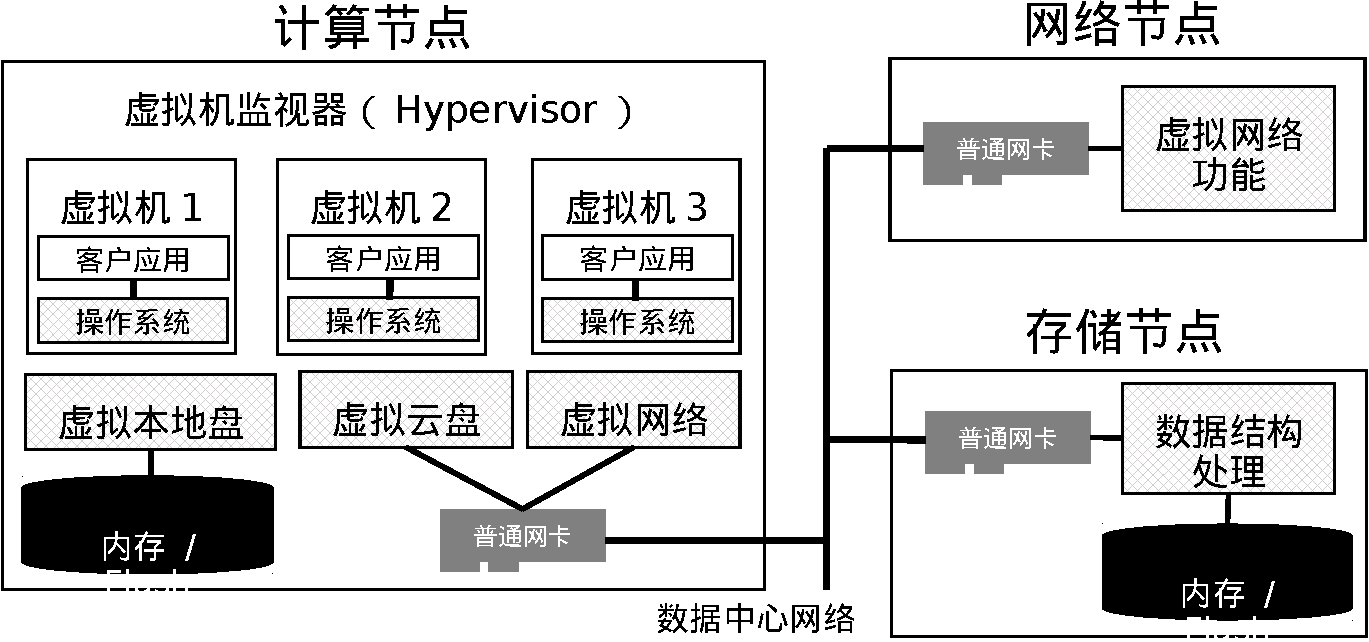
\includegraphics[width=0.8\textwidth]{figures/virt_arch.pdf}
	\caption{虚拟化的数据中心架构。}
	\label{background:fig:virt-architecture}
\end{figure}

\section{国内外研究现状}




第二章提炼 2 页

\section{本文的研究内容和贡献}



\begin{figure}[htbp]
	\centering
	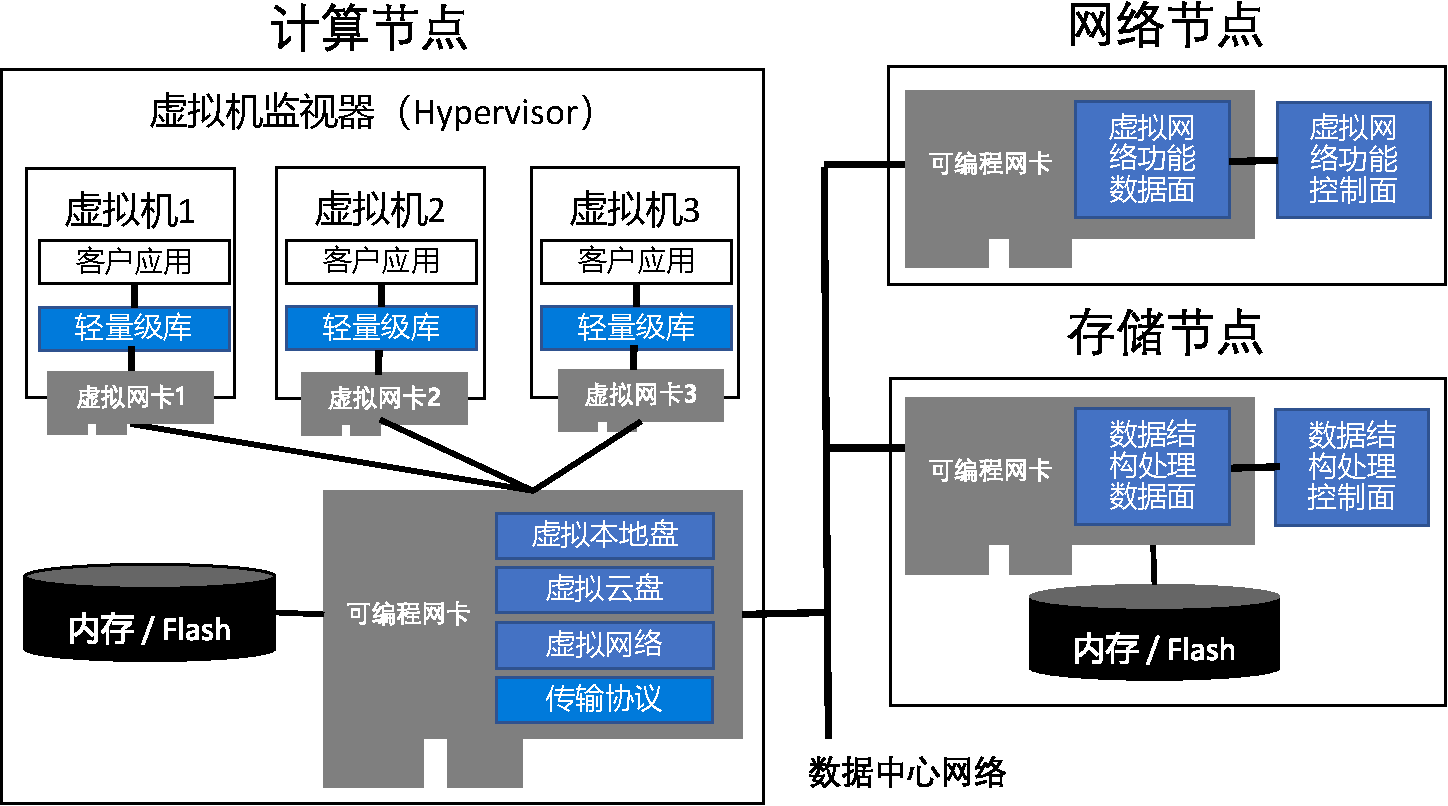
\includegraphics[width=0.8\textwidth]{figures/accel_arch.pdf}
	\caption{基于可编程网卡的数据中心系统总体架构。}
	\label{arch:fig:accel-arch}
\end{figure}

摘要的扩充,第三章提炼 2 页

\section{论文结构安排}

本论⽂的内容结构安排如下:
第 1 章为绪论。
第 2 章介绍了数据中心的背景知识和硬件的发展趋势,分析了可编程网卡的四种架构,并调研了可编程网卡在数据中心的应用。
第 3 章提出了基于可编程网卡的高性能数据中心系统架构。
第 4 章提出用可编程网卡加速云计算中的虚拟网络功能。为了简化FPGA编程,提出了首个适用于高速网络数据包处理、基于高级语言的模块化FPGA编程框架ClickNP。
第 5 章提出用可编程网卡加速远程数据结构访问,并设计实现了一个高性能内存键值存储系统 KV-Direct。
第 6 章提出用可编程网卡和用户态运行库相结合的方法为应用程序提供系统原语,并设计实现了一个用户态套接字系统 SocksDirect。
第 7 章总结全⽂并展望未来研究方向。
%!TEX root=main.tex
\chapter{数据中心与可编程网卡概论}
\label{chapter:background}

本章介绍全文的背景和相关工作。第 1 节回顾数据中心的发展历史,展望数据中心的未来趋势,提出数据中心的性能开销与挑战,以及性能优化的可能方向。第 2 节综述数据中心计算、内存、存储和网络互连系统硬件的发展趋势。第 3 节讨论基于专用芯片、网络处理器、通用处理器、FPGA 的四种可编程网卡架构。第 4 节调研可编程网卡在微软 Azure、亚马逊 AWS 等数据中心的部署。

\section{数据中心的性能挑战}
\label{background:sec:challenge}

\subsection{数据中心的过去、现在与未来}

从 20 世纪 50 年代计算机的诞生到 90 年代互联网兴起前,人类的算力大部分用于高性能计算、数字化企业和个人计算机(PC),其产生的数据大多存储在一个个信息孤岛上。需要处理大量信息的大型机乃至超级计算机一般采用软硬件一体化系统,即软硬件是由同一个公司团队开发的。由于采用了高速硬件互连、硬件冗余,这些系统往往同时具备高性能和高可靠性,但成本随系统规模的扩大急剧增加。为了充分利用昂贵的计算机,虚拟化的概念应运而生。其中 20 世纪 50 至 60 年代的分时系统 \cite{strachey1959time,amdahl1964architecture} 实现了多个用户任务分时复用硬件,发展成为 70 年代 UNIX 等现代操作系统 \cite{bach1986design} 的前身。20 世纪 70 至 90 年代,虚拟机监视器(Virtual Machine Monitor,VMM)进一步实现了多个操作系统分时复用硬件 \cite{popek1974formal,agesen2010evolution},为云计算的发展做了技术准备。

20 世纪末,连接信息孤岛的搜索引擎拉开了互联网时代的序幕。数据中心不仅需要搜集、处理和索引海量信息,还需要实时响应大量用户的信息检索请求。传统的超级计算机、大型机和企业级存储不仅成本高昂,也无法满足海量信息存储和用户请求处理的可扩放性。为此,Google 提出用普通商用服务器组建可扩放的数据中心,用软件来实现存储的分区和冗余、用户请求的分派,在相对不可靠的硬件基础上组建起容错的系统 \cite{dean2008mapreduce}。

这些普通商用服务器之所以成本较低,是因为它的架构与大量商用的个人计算机(PC)类似,CPU、内存、主板、硬盘、网卡等组成部分都是标准组件,由各个专业公司独立设计实现。操作系统、数据库、Web 服务器等软件也是标准化的,或者由专业公司开发,或者是开源软件。产量大的标准组件能更好地平摊研发、流片等一次性工程费用(Non-Recurring Engineering,NRE),从而降低标准组件的价格。由标准组件构成的系统虽然降低了数据中心的软硬件成本,但也给标准组件的开发者施加了限制:大家需要遵守标准组件之间的接口和协议,只能在自己的边界内创新。数据中心系统的搭建者则只能像搭积木一样组合标准组件,而很难通盘考虑、全局优化。

21 世纪的第一个十年,互联网的发展让越来越多的企业需要提供 24 小时运行的网络服务,互联网数据中心(Internet Data Center,IDC)托管服务逐渐兴起。然而,IDC 托管需要客户事先购买服务器硬件,并需要运维人员维护,有较高的资产成本(capex)和运营成本(opex)。很多企业的网络服务一方面具有较高的季节性(如亚马逊的黑五促销),因此在闲时大量的计算资源被闲置;另一方面数据和用户规模的扩张很快,给购买硬件和 IDC 选址带来了时间压力。为此,虚拟机托管服务提供了按需租用的虚拟机资源,实现了服务器资源按 CPU 核的切片和在不同客户间的分时复用,也便于客户内部运维人员的管理和调度。

云计算是虚拟机托管服务的升级版,标志性的变革是计算和存储的解耦。虚拟主机托管服务把一台主机上的计算和存储资源分片成多个虚拟机,一旦主机的硬件或虚拟化软件(hypervisor)发生故障,虚拟机也就停机,其中的数据还有丢失的风险。在云计算中,虚拟机的存储资源在分布式存储系统中有多个副本,从而计算节点发生故障时可以从其他计算节点重启虚拟机,存储节点的故障则一般对客户透明。计算和存储的解耦不仅大大提高了服务可用性和数据安全性,也方便了虚拟化软件升级和虚拟机热迁移。


\textbf{云的趋势。摩尔定律。}

\textbf{10 年前,大规模数据处理。}

\textbf{5 年前,深度学习开始兴起。}

\iffalse

\textbf{产品容易传输、各行各业都能用到的基础设施会云化……}
电力作为工业和城市的基础资源,早期也是由需要电的工厂、学校等自己购买发电机来发电,逐渐才形成今天庞大而复杂的电力系统,由发电、输电、变电、配售电等多个标准化的环节构成,客户只需要按需租用电力资源。
计算机作为信息社会的基础设施,自然也不例外。从早期的客户自己购买和运维计算机、操作系统、应用程序,到今天被称为云计算的按需租用计算、存储和网络资源甚至更上层的应用服务。
未来,对提供互联网服务的公司和个人而言,自建数据中心、购买和运维服务器就像自建发电厂、购买和维护发电机一样,在大多数场景下成本很高且没有必要。

随着云计算的发展,工程师们重新获得了在计算机全栈(full-stack)上创新的机会。在云计算平台中,软件和硬件的环境都由服务商控制,在达到了一定的规模以后,各种形式的定制(customization)都成为可能。只要能够提高性能,降低价格,增强竞争力,云服务商有足够的动力去定制芯片,改变网络协议,改变服务器架构,更改操作系统,甚至重新编写应用程序。下一代云平台想要保持竞争优势,除了完善的软件栈外,还必须在体系结构上创新。像过去一样完全使用现成部件(off-the-shelf components)就可以构建有竞争力的公有云平台的时代已经一去不复返了。而在不远的未来,这些云端体系结构的创新必然会向下流动,对未来私有云、企业服务器甚至个人计算机和移动计算的体系结构都会带来深远影响。
\fi

\textbf{云计算和 5G 需要虚拟化,需要灵活性、可编程性和可调试性}


\textbf{计算粒度:从物理机,到虚拟机,到容器(基于容器的微服务),到函数 Granular Computing}

例如,微信有超过 3000 个微服务运行在超过 2 万台服务器上。入口层的微服务每天响应 100 亿至 1000 亿次用户请求,而每个用户请求会在系统内部触发更多的微服务请求,因此整个微信后端每秒需要响应数以亿计的微服务请求 \cite{zhou2018overload}。

加州大学伯克利分校对无服务器计算(serverless computing)的预测报告 \cite{jonas2019cloud} 表明,尽管无服务器计算的范式有诸多优势,也是各大云服务商争相推广的新服务,但由于云存储的性能问题和临时存储服务的缺失,很多类型的应用使用无服务器计算的性能和成本不理想。


\subsection{虚拟化的数据中心架构}

中国系统科学的先驱钱学森老先生说: ``任何事物的开始总是比较简陋的,只有在不断发展的过程中才逐渐完善,逐渐形成一整套复杂而又有机地结合着的体系。'' \cite{qianxuesen}
例如,火车和飞机作为交通工具,早期没有火车站、机场,没有车辆段、修配厂等辅助设施,更没有铁路行车信号、空中交通管制和相关的法律法规。
云计算的发展也是相似的。
使用 OpenStack 开源软件中的一部分组件,我们就可以轻松地搭建出一个由管理、计算、存储节点构成的私有云,满足实验室或小型公司内部的搭建 Web 服务、共享文件、OA 系统等需求。
然而,如果是针对学校或中型公司的需求,就需要支持不同部门之间的隔离……需要 VPC 的概念,网络虚拟化,网络节点承载网络功能……
如果需要大数据处理,深度学习,需要不同硬件,高性能互连……还需要共享数据结构存储……
发展到现代的公有云,提供了上百种不同层次的服务和解决方案。
\textbf{补全}

尽管现代的云计算平台服务多样、结构复杂,其基础也是计算机所必需的计算、内存、存储、网络和互连资源。
在目前基于机架服务器的数据中心中,由于计算设备和内存间高带宽、低延迟的需求,计算和内存一般是绑定在同一台服务器中的。
为了高效地共享计算、存储和网络互连资源,这些资源都被虚拟化,由池化的机架服务器节点提供。
庞大而又复杂的云服务体系是由计算节点池、网络节点池、存储节点池和管理节点池构成的。

\begin{figure}[htbp]
	\centering
	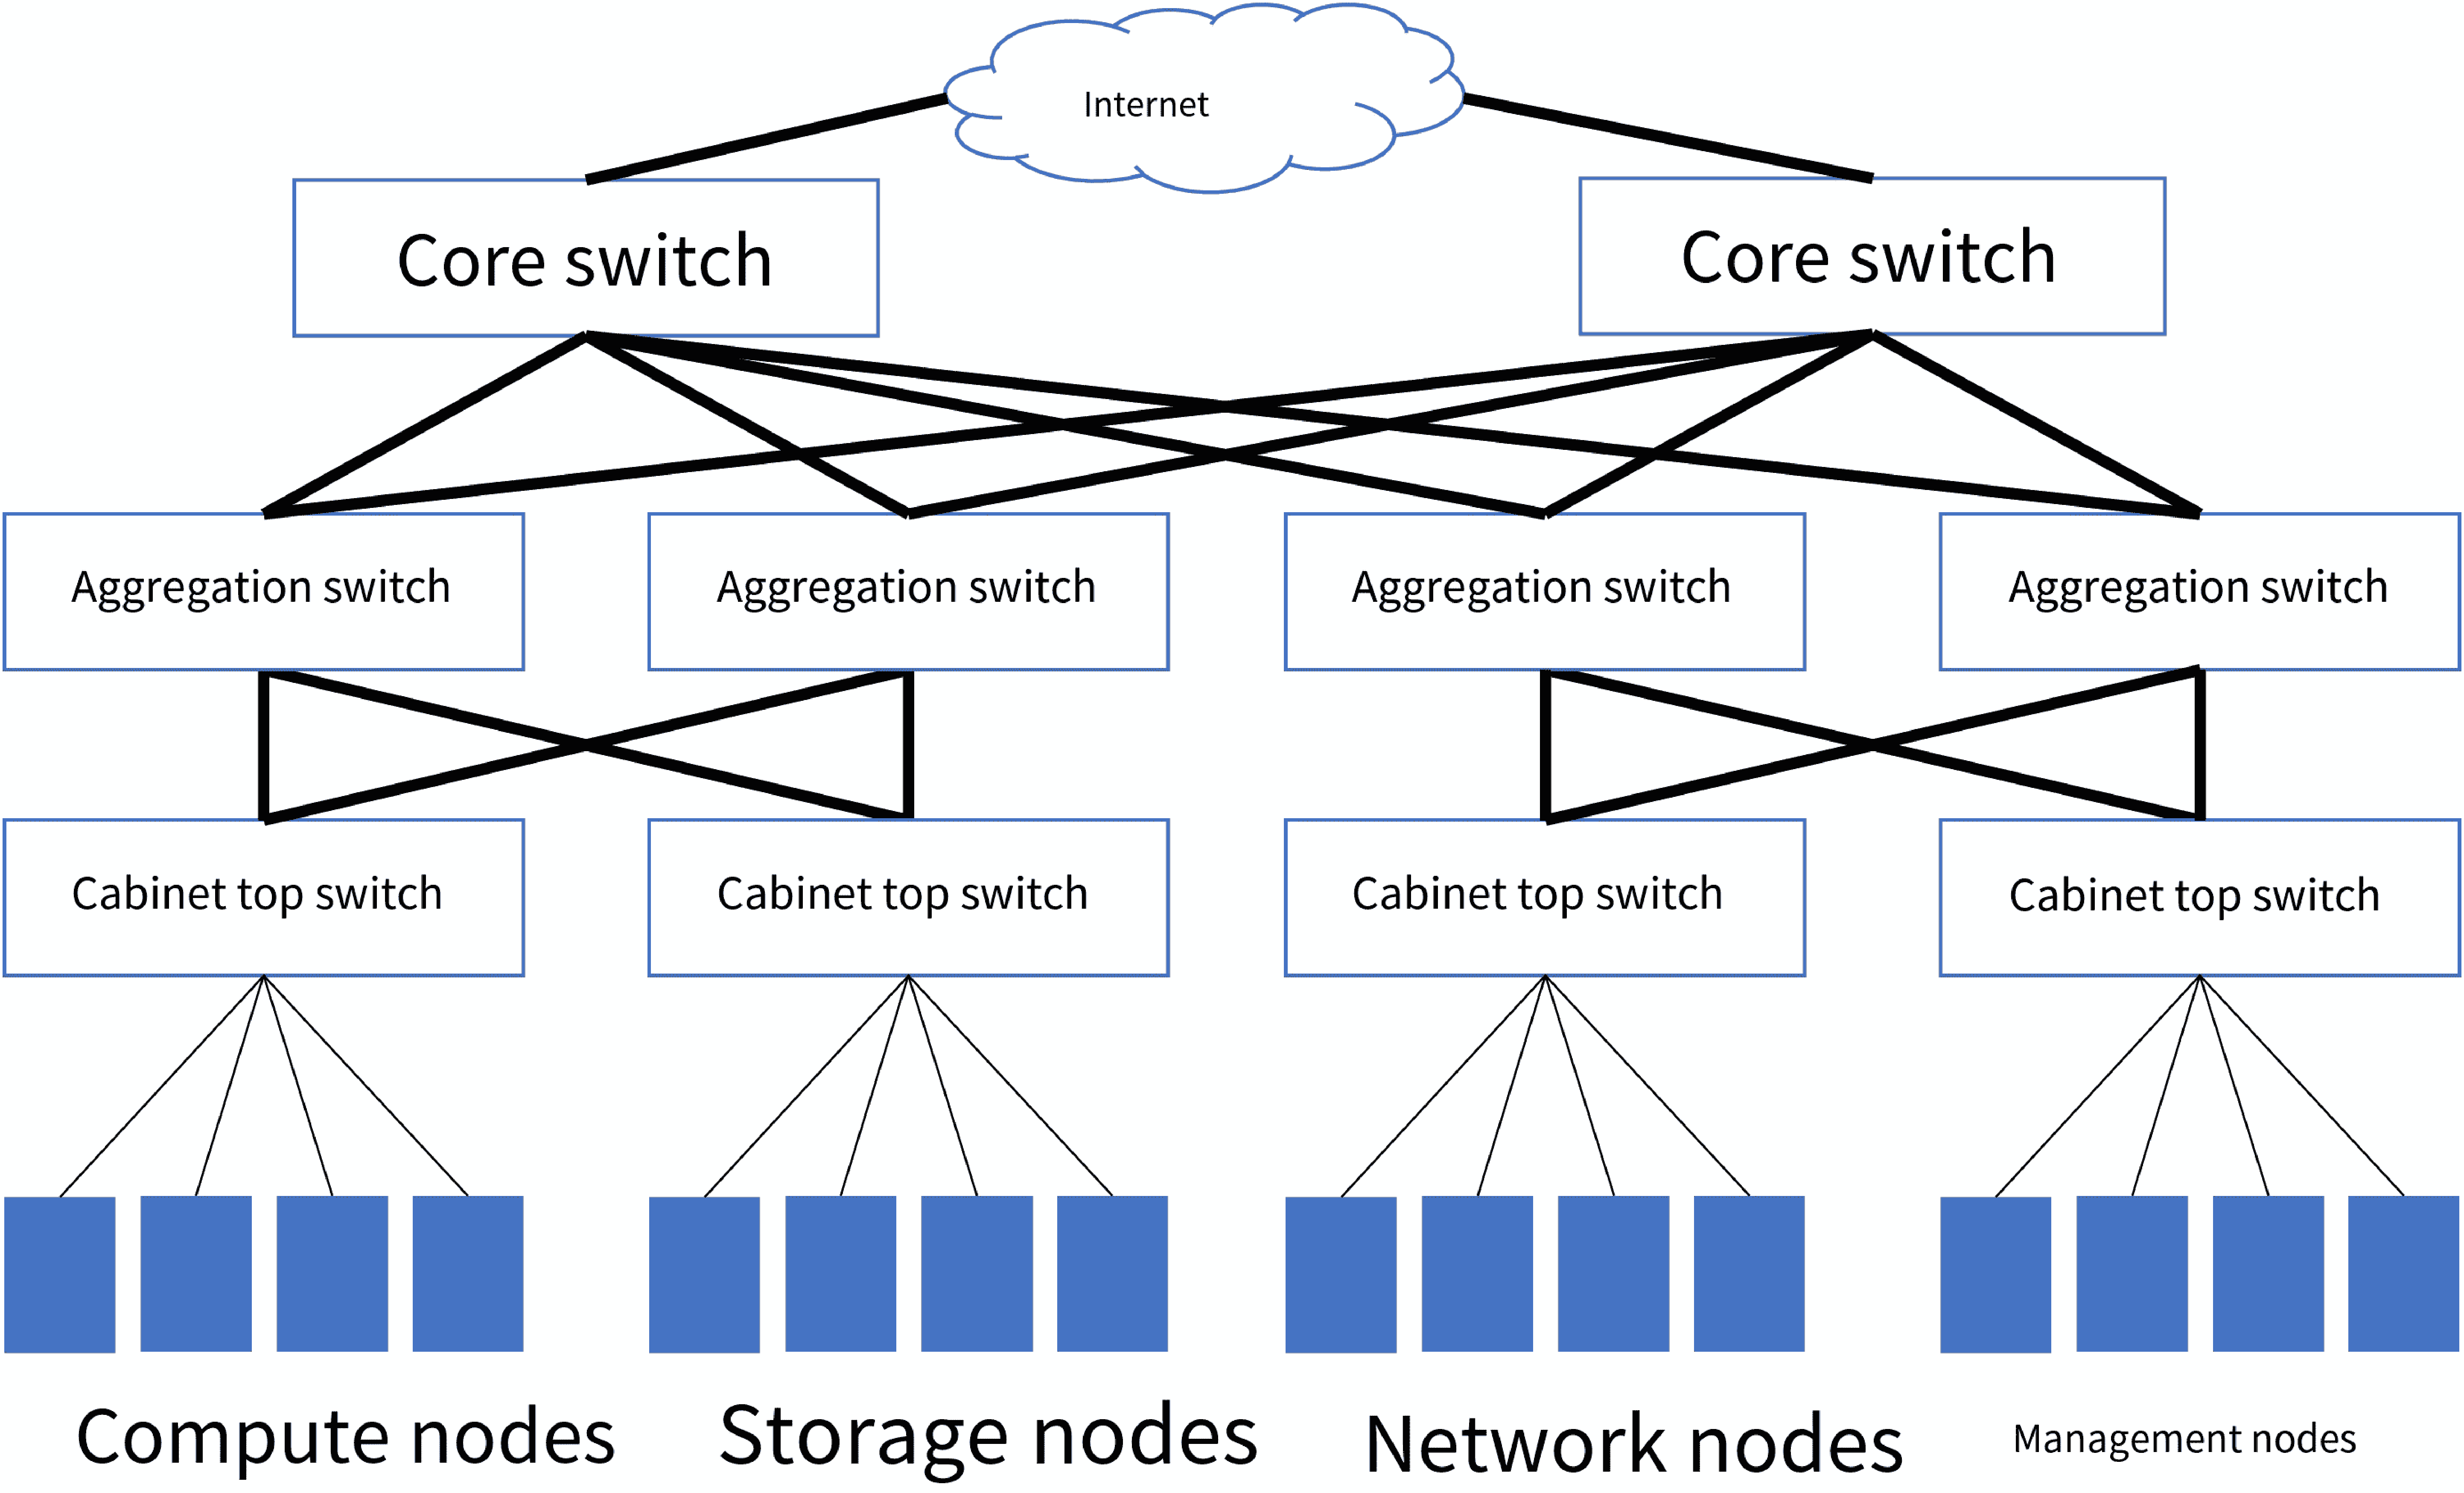
\includegraphics[width=0.6\textwidth]{figures/DC_arch.pdf}
	\caption{数据中心架构。}
	\label{background:fig:cloud-architecture}
\end{figure}

\begin{figure}[htbp]
	\centering
	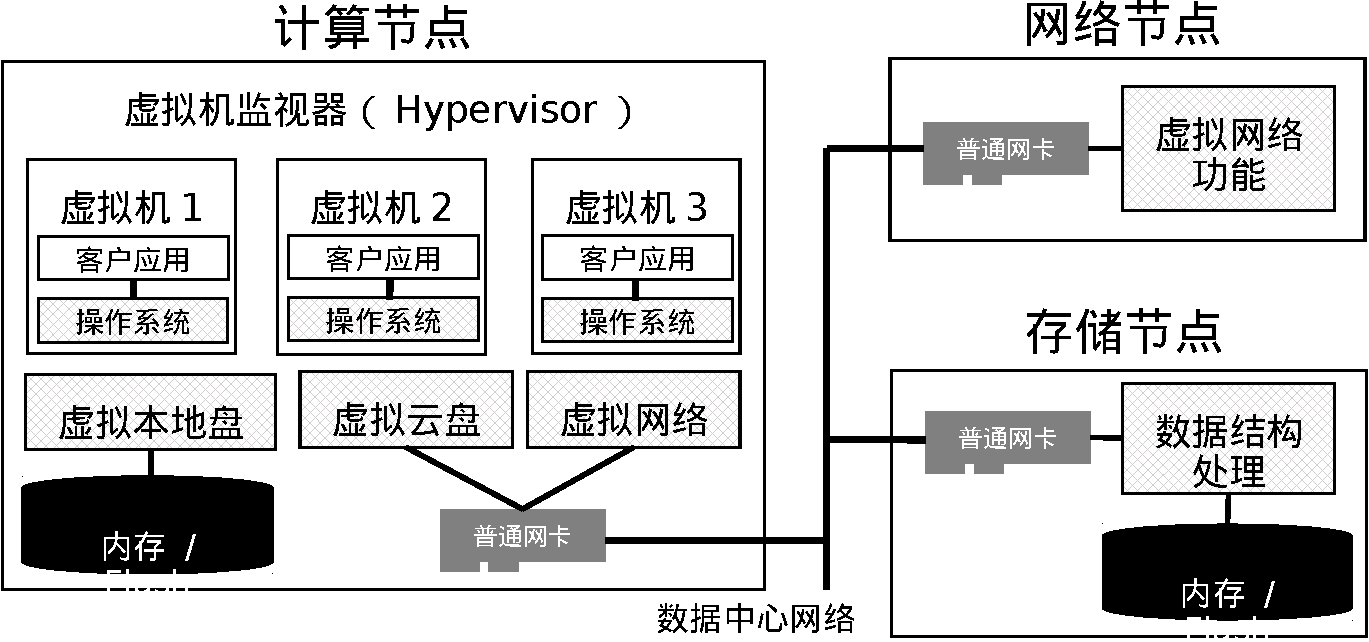
\includegraphics[width=0.8\textwidth]{figures/virt_arch.pdf}
	\caption{虚拟化的数据中心架构。}
	\label{background:fig:virt-architecture}
\end{figure}


\subsubsection{虚拟网络}

除销售虚拟机外,销售基础架构即服务(IaaS)的云供应商必须提供丰富的网络语义,例如具有客户提供的地址空间的私有虚拟网络,安全组和ACL,虚拟路由表,带宽计量,QoS等。 

计算节点上虚拟网络的数据面可以用匹配-操作表(Match Action Table)来描述,理论上可以在商用网络交换机上实现。
2007 年,斯坦福大学提出的 OpenFlow \cite{mckeown2008openflow} 统一了不同厂商交换机的控制面接口,从而可以用软件来对网络进行编程,即软件定义网络(Software Defined Networking,SDN)。
为了支持软件定义网络的控制面,Onix \cite{koponen2010onix} 提出了一个大规模交换机的控制框架,Frenetic 等编程语言 \cite{voellmy2010nettle,foster2011frenetic} 提出用函数式响应型编程(Functional Reactive Programming,FRP)的范式简化控制面事件处理,Covisor \cite{jin2015covisor} 实现了控制面的虚拟化。
随着交换机的可编程性越来越高,用软件自顶向下地定义交换机的数据面转发行为成为可能,而不是像 OpenFlow 那样自下而上地适配交换机的固定功能。

为此,2013 年,斯坦福大学提出了 P4 \cite{bosshart2014p4},提供可编程的数据包解析、有状态的匹配-操作流水线等编程抽象。
学术界提出了 P4 语言在可编程交换机芯片 \cite{bosshart2013forwarding}、可编程网卡 \cite{kaufmann2016high}、FPGA \cite{wang2017p4fpga}、CPU 虚拟交换机 \cite{shahbaz2016pisces} 上的多种实现。
工业界的 Barefoot Tofino 交换机芯片 \cite{barefoot-tofino}、Mellanox Connect-X 网卡 \cite{mellanox}、基于 FPGA 的 Xilinx SDNet 网络处理器 \cite{xilinx-p4} 等也支持了 P4 语言。

然而,基于网络交换机的虚拟网络在云数据中心中有两个根本挑战。
首先,虚拟网络的语义非常复杂,而且变化太频繁,以至于固定功能的传统交换机硬件更新的速度很难匹配需求变更的速度。
其次,一台柜顶交换机连接了数十台机架服务器,一台机架服务器又可以虚拟化出数十台虚拟机,因此交换机需要支持至多上千台虚拟机的数据面封装和转发规则,现有商用交换机芯片的查找表容量不足。
为此,微软提出了类似 P4 的 VFP 编程抽象 \cite{firestone2017vfp} 以支持基于主机的软件定义网络,在虚拟交换机软件中实现虚拟网络。基于主机的虚拟网络可以很好地随计算节点服务器的数量扩放,并保持了物理网络的简单性。

在这种基于虚拟交换机的网络虚拟化模型中,进出物理设备的所有网络I / O都专门在管理程序的主机软件分区中执行。 VM发送和接收的每个数据包都由主机网络堆栈中的虚拟交换机(vSwitch)处理。 接收数据包通常涉及管理程序将每个数据包复制到VM可见缓冲区,模拟到VM的软中断,然后允许VM的OS堆栈继续进行网络处理。 发送数据包类似,但顺序相反。 与非虚拟化环境相比,这种额外的主机处理:降低性能,需要对权限级别进行额外更改,降低吞吐量,增加延迟和延迟变化,并提高主机CPU利用率。

如图 \ref{background:fig:network-perf-trend} 所示,数据中心网络性能的提升速度远远超过通用处理器,在 10 Gbps 网络中只需要一个 CPU 核,而在现在的 40 Gbps 网络中就需要 5 个左右的 CPU 核,而在未来的 100 Gbps 网络中甚至需要 12 个 CPU 核。这就带来了 ``数据中心税''。





\begin{figure}[htbp]
	\centering
	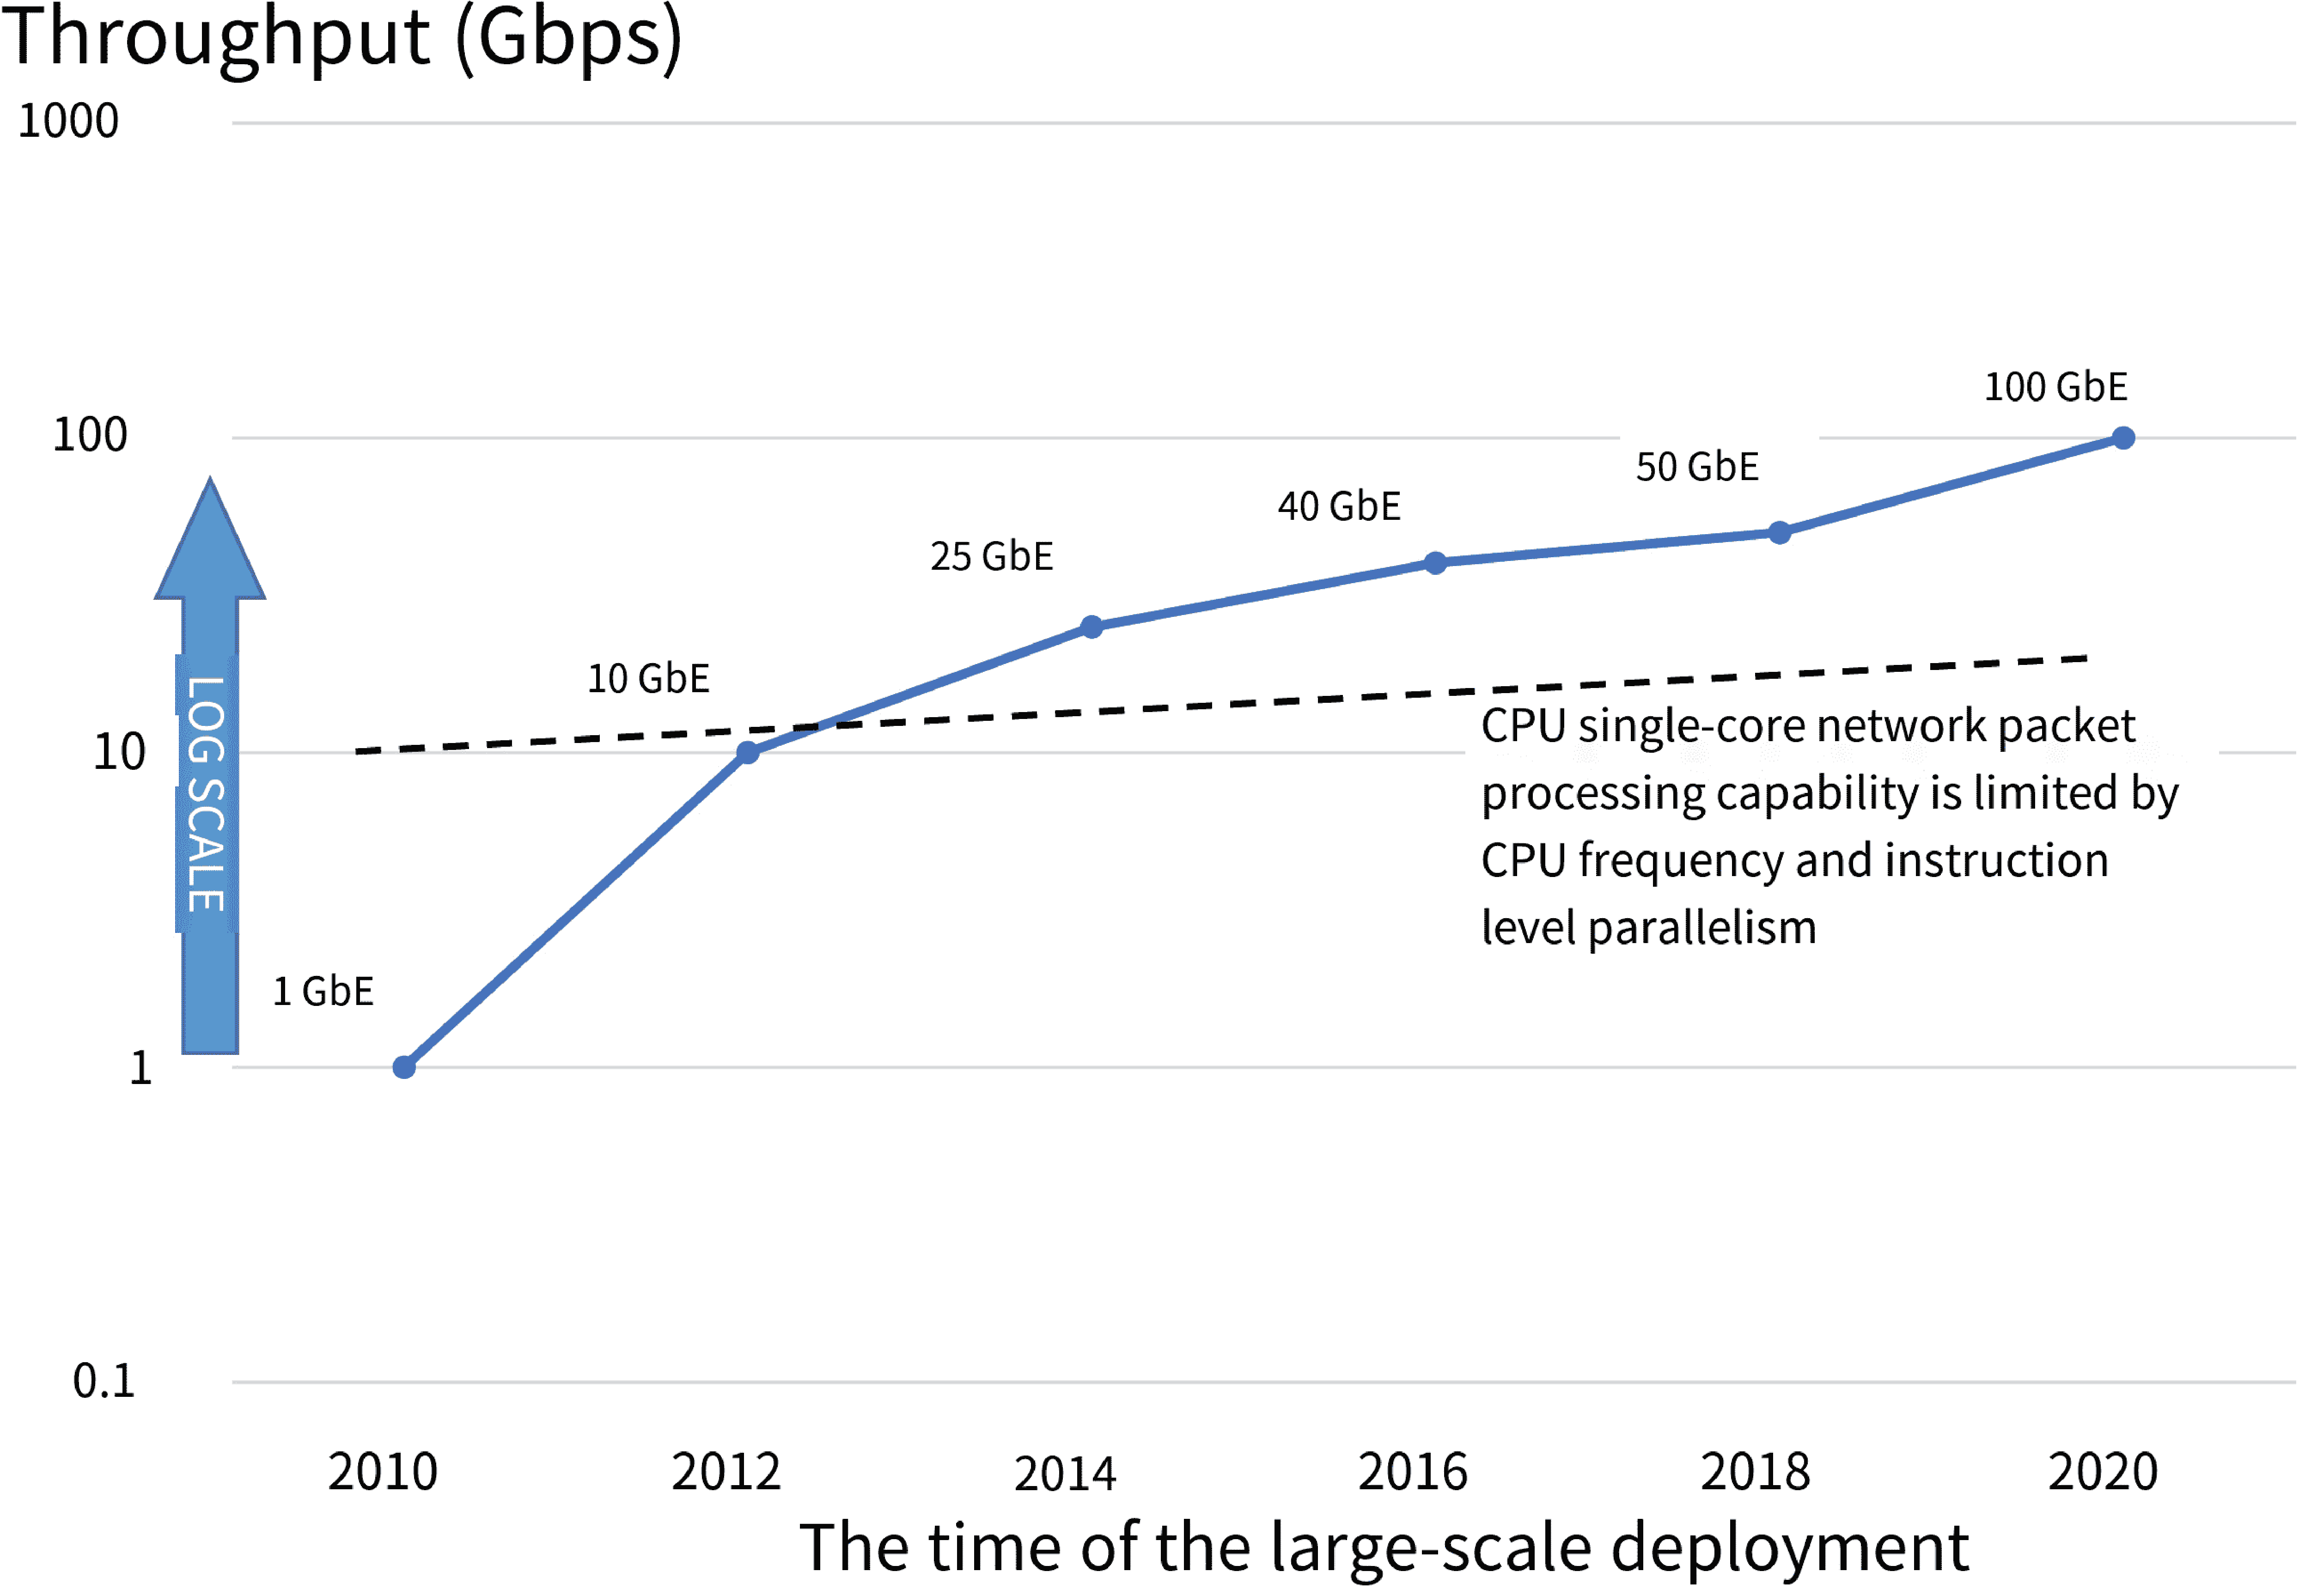
\includegraphics[width=0.6\textwidth]{figures/network_perf_trend.pdf}
	\caption{数据中心网络性能的提升速度远超 CPU。}
	\label{background:fig:network-perf-trend}
\end{figure}


\subsubsection{网络功能}

如图 \ref{background:fig:network-architecture} 所示,两个计算节点上的客户虚拟机之间通信时,经常需要经过一系列网络功能。相比计算节点上的虚拟网络,网络节点上的网络功能就复杂得多。

例如,可扩展的L4负载平衡器 \cite{ananta}

P4 的编程灵活性不足以实现。


\begin{figure}[htbp]
	\centering
	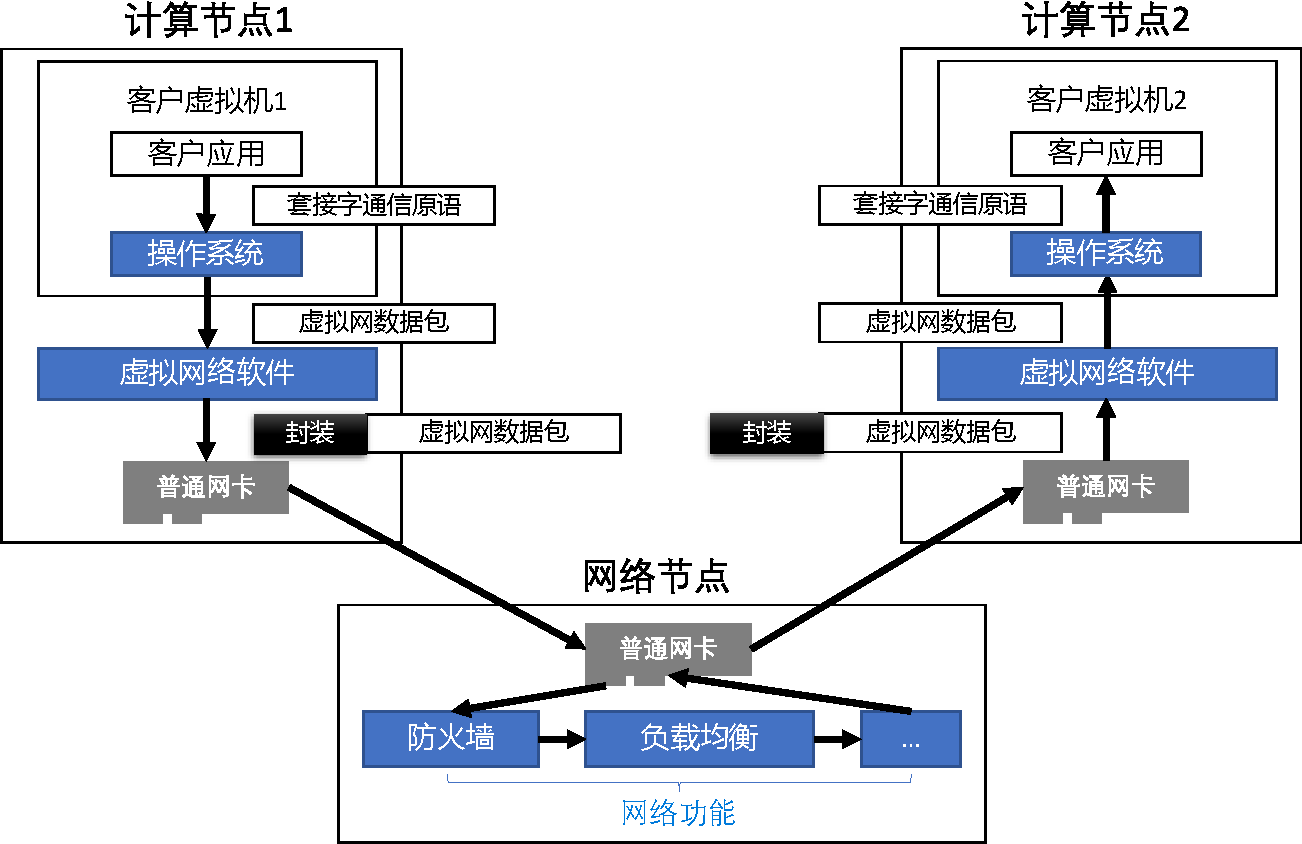
\includegraphics[width=0.8\textwidth]{figures/VPC_arch.pdf}
	\caption{数据中心虚拟网络架构。}
	\label{background:fig:network-architecture}
\end{figure}




Click \cite{kohler2000click} 提出了模块化的网络编程框架。近年来,ClickOS \cite{martins2014clickos} 和 NetBricks \cite{netbricks} 提出了基于 CPU 的

E2 \cite{palkar2015e2} 网络功能

\subsubsection{虚拟存储}




\begin{figure}[htbp]
	\centering
	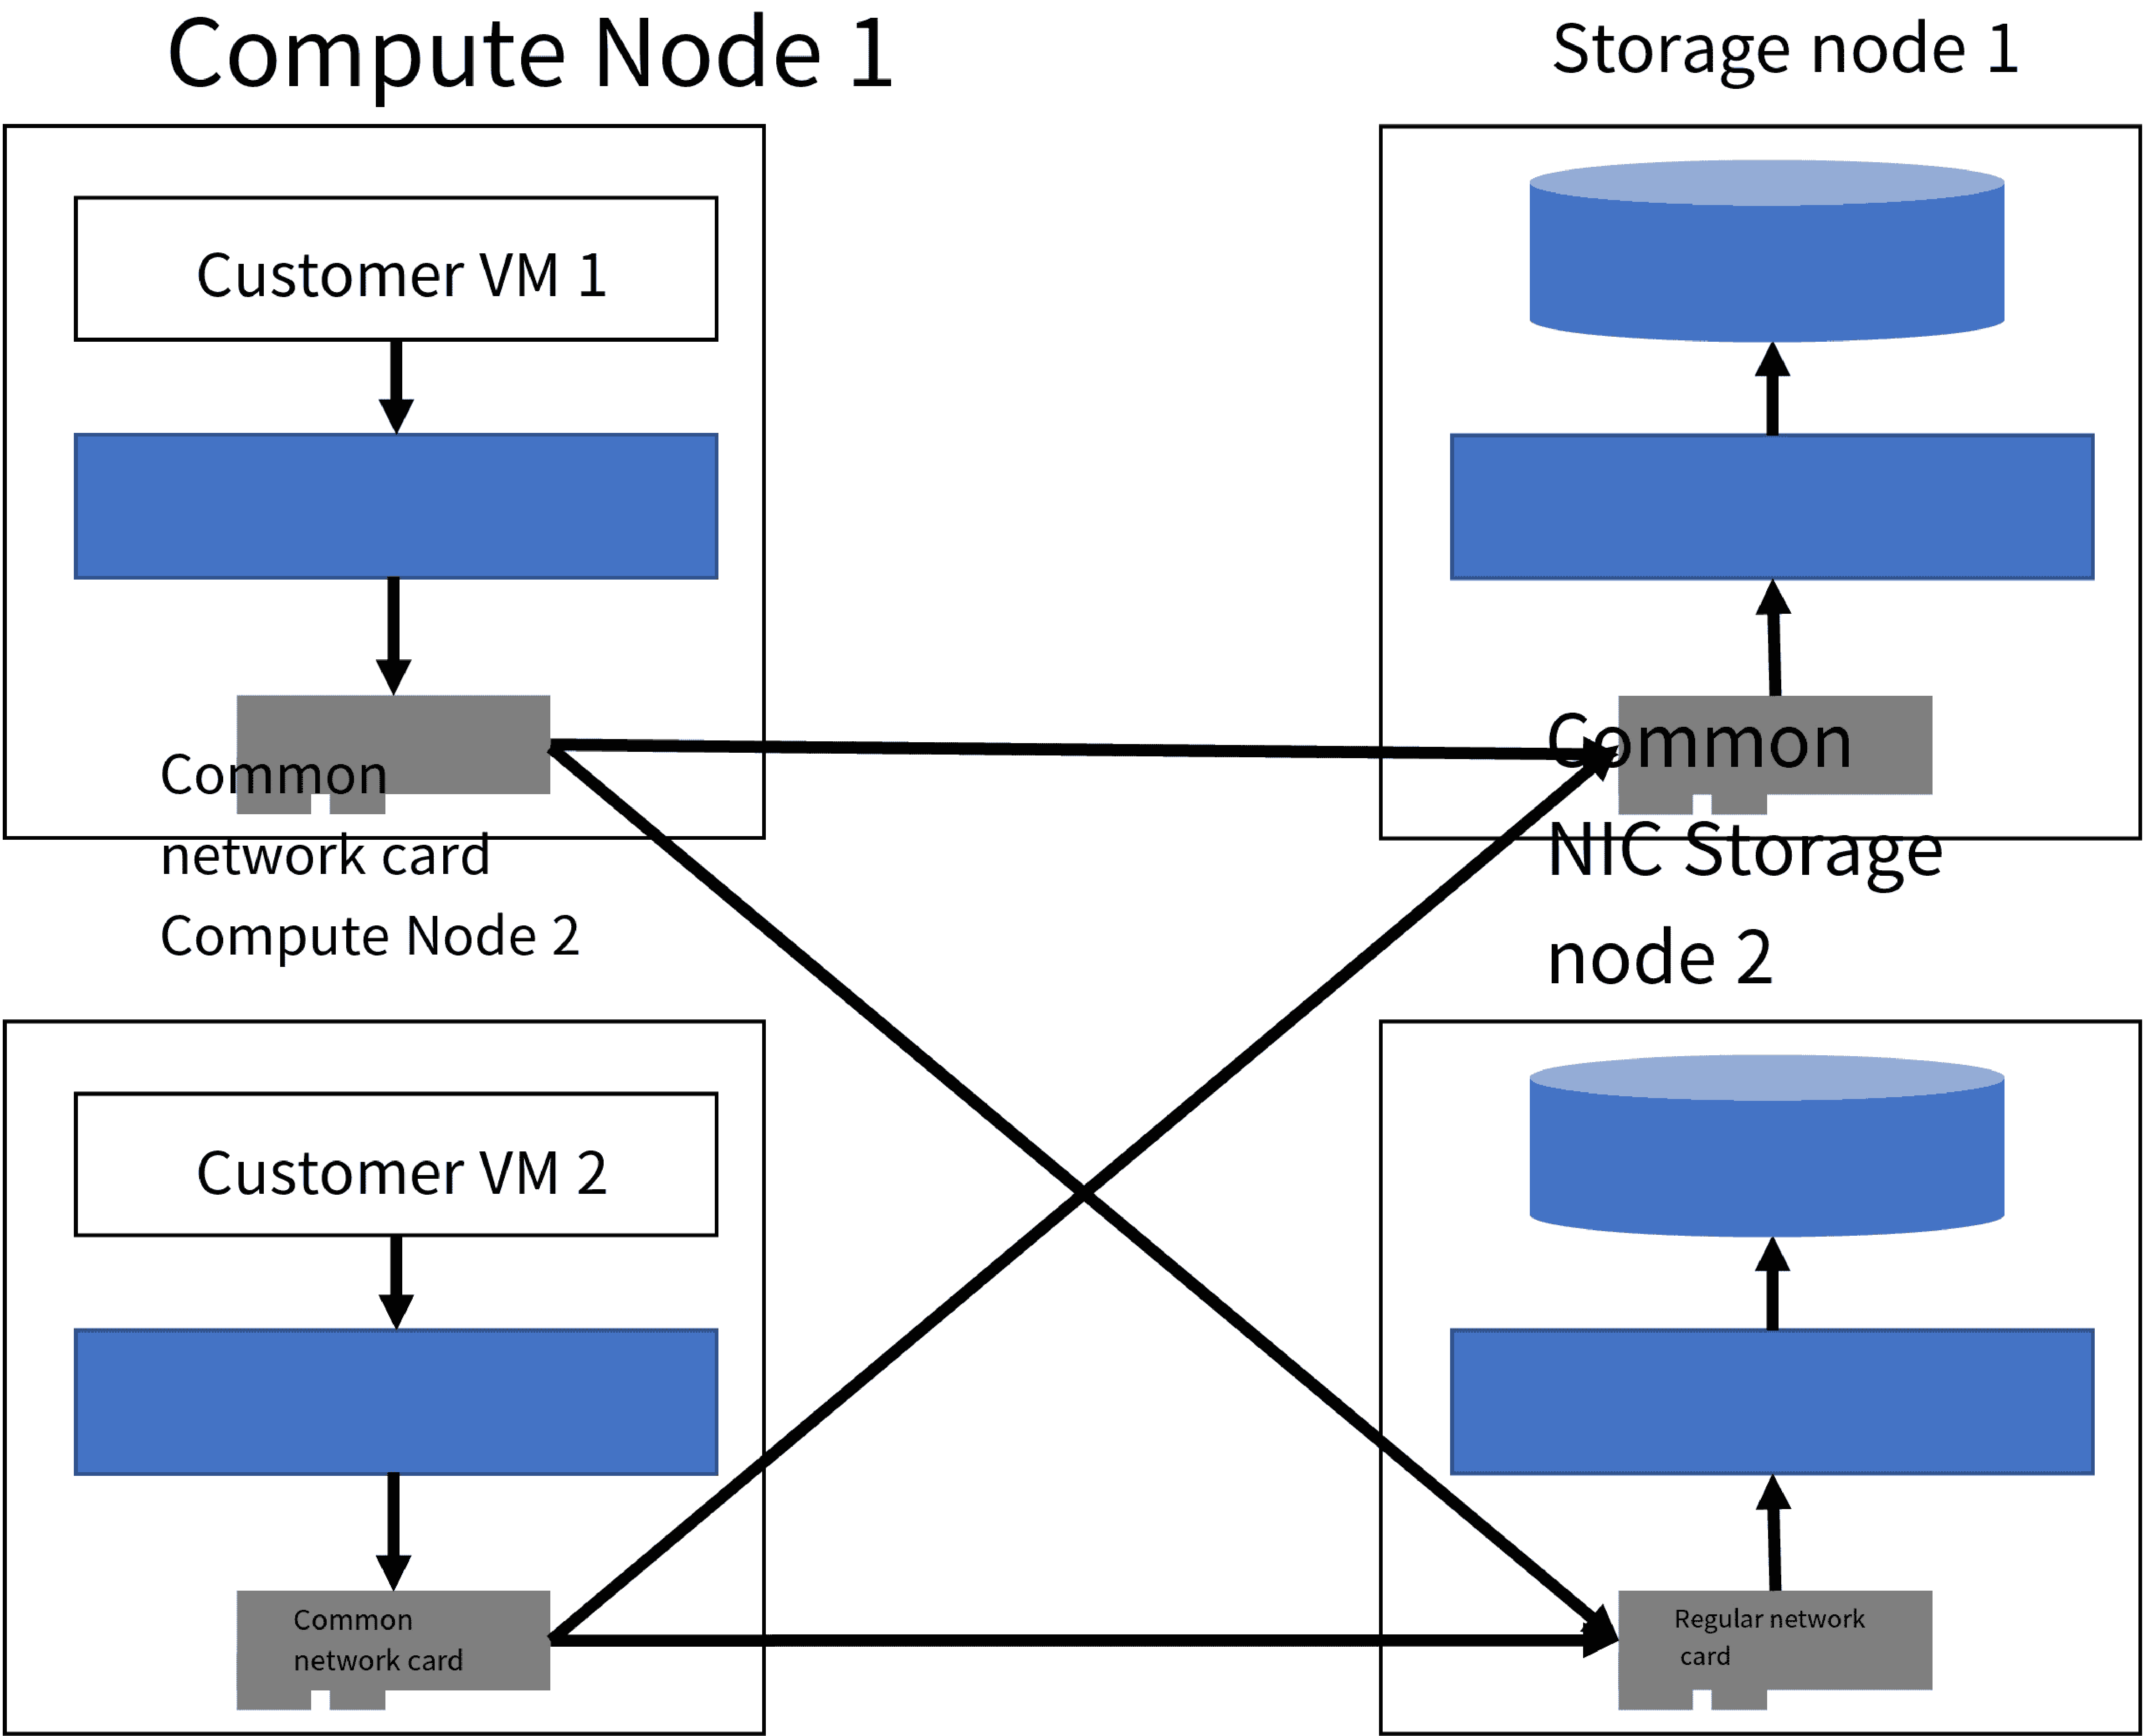
\includegraphics[width=0.6\textwidth]{figures/storage_arch.pdf}
	\caption{数据中心云存储的简要架构。}
	\label{background:fig:storage_arch}
\end{figure}

块存储,本地盘

对象存储,文件存储

临时存储(Serverless computing)

由于云存储的物理存储跟计算节点是分离的,需要把数据从存储节点通过网络搬运过来,还要进行压缩和加密。




\subsection{数据中心功耗的挑战}

如今的一个大型数据中心可以占据几个足球场的面积,容纳数十万台服务器,消耗几十甚至上百兆瓦的电力,相当于一个小型工业城镇的耗电量。据统计,2018 年全球数据中心约消耗 416 太瓦时的电力,相当于 2\% 左右的全球电力能源 \cite{datacenter-energy},占整个信息与通信产业(ICT)能耗的约 33\%。据预测,2025 年,信息与通信产业将消耗 17.8\% 至 20.7\% 的全球电力能源,其中数据中心占 43\% 至 58\% \cite{power-consumption},这意味着 2025 年数据中心将消耗全球电力的约 10\%。因此,数据中心的性能与效率不仅关系到互联网公司的资产和运营成本,还关系到信息产业的未来。

为什么能源问题对信息产业的未来如此重要呢?
1961 年,钱学森预言,``长远以来人们就有在宇宙空间飞行的愿望……星际航行将是科学技术在 20 世纪后半叶中最突出的成就。'' \cite{qianxuesen}
可惜,不同于钱老等大科学家和阿瑟·克拉克等大科幻作家的预言,星际航行的探索尽管推动了众多科学和工程技术的大发展,但由于能源和材料的限制,至今没有成为一项大众技术。
而信息和通信技术(ICT)由于摩尔定律所预言的指数级性能提升,成为 20 世纪末以来最为耀眼的科技新星。

由于信息是无形的,我们可以通过把信息的存储和处理单元做得越来越小来提升单位面积集成电路的存储和处理单元数量,从而提升单位面积集成电路的性能。这也是摩尔定律的原始表述。
更为深刻的是 Dennard 缩放定律 \cite{dennard1974design},即集成电路的性能在不消耗更多能源和面积的情况下能够每两年翻倍。
它的理论基础是每两年采用一代新的半导体工艺,晶体管尺寸缩小 30\%,从而芯片面积缩小 50\%。为了保持电场的恒定,电压随晶体管尺寸同比例降低了 30\%。与此同时,由于芯片尺寸缩小了,延迟降低了 30\%,时钟频率就可以提升 40\% \cite{borkar1999design,borkar2011future}。
在那个年代,集成电路的动态功耗占了功耗的主要部分,其与电容、电压的平方和频率成正比,从而可以计算出功耗降低了 50\%。
按照这个理想模型,每两年集成电路的面积和功耗都减半,就可以在原有的面积和功耗下塞进两倍数量的晶体管,而且时钟频率还提高到了 1.4 倍。
对于冯·诺伊曼体系结构的单线程微处理器,这些增加的晶体管主要用于更大的缓存、更复杂的流水线、超标量、乱序执行、寄存器重命名、分支预测等,以提高每时钟周期所能执行的指令数。
根据 Pollard 经验定律 \cite{pollackpollack},每时钟周期的计算能力大约与晶体管数量的平方根成正比。
单位时间的算力等于时钟频率乘以每时钟周期的算力,因此每两年微处理器的性能提升到 2 倍,还不消耗更多的能源和面积。

信息系统性能提升的速度在处理宏观有形物体的其他行业是难以想象的。
1976 年,协和式客机的速度就突破了音障,然而它因为油耗太高而没有经济性。现代客机与 50 年前的多数客机一样,仍然以亚音速飞行。
而从普速火车到高铁的大量系统创新,也只把运营速度提高到了 2 倍多。
目前,人类的主要能源来源是化石能源,由于其使用成本和环境影响,在新能源技术取得重大突破前,能源仍然是各行各业发展的重要制约因素 \cite{energy}。
相比数据中心,移动终端和物联网设备对功耗更敏感,因为电池的能量密度提升缓慢,而这些设备对体积和重量很敏感。

不幸的是,进入 21 世纪以来,摩尔定律和 Dennard 缩放定律的红利正在逐渐消失。
首先,随着集成电路特征尺寸的缩小,电压也随之降低。但控制晶体管的阈值电压越低,晶体管的漏电流就会迅速增长,成为集成电路功耗的重要组成部分。
为了控制漏电流,阈值电压不仅不能降低,甚至需要比前一代集成电路有所提高 \cite{borkar1999design}。
因此,每一代新的半导体工艺,每晶体管的功耗不会像预期的那样降低一半。
其次,由于每晶体管的面积缩小一半,功耗却没有降低这么多,单位面积集成电路的功耗就会升高。
目前 100 平方毫米芯片的功耗大约是 65 瓦 \cite{borkar2011future},成为人类最高功率密度的可控设备之一,单位体积的功率密度甚至与航空发动机相当。因此,芯片的散热问题成为制约集成电路规模的主要因素。
再次,对于同一个集成电路,在允许的范围内,为了提高一倍的性能而把时钟频率提高一倍,电压就要相应提高一倍来降低晶体管的翻转延迟,因此功耗大致与时钟频率的三次方成正比。
由于散热的限制,集成电路的时钟频率也受到限制,靠 ``超频'' 来大幅提升集成电路性能是不现实的。
最后,目前 7 nm 半导体工艺已经量产,而硅原子的半径为 0.1 nm。
随着集成电路的特征尺寸越来越接近原子尺寸,量子效应不可忽略,给光刻技术带来了很大的技术挑战 \cite{borkar2011future}。
事实上,约 2010 年以来,集成电路特征尺寸的缩小已经明显放缓,不再能保持两年一代的速度。
综上,在当前的半导体技术框架下,单位面积集成电路的性能已经不再能维持两年提升一倍的速度,而且性能的提升也意味着功耗的提升,``免费的午餐'' 结束了。

在通信技术方面,信道编码从相对低效的汉明(Hamming)码和格雷(Golay)码,发展到卷积码,再到接近香农极限的 Turbo 码和从故纸堆中翻出来的 LDPC 码,以及理论上达到香农极限的 Polar 码,在物理信道和信噪比不变的前提下,通信系统的吞吐量逐渐接近香农极限。
事实上,Turbo 码在 HSPA、LTE、WiMAX 等无线通信标准中被广泛采用,LDPC 码被用于 5G eMBB 数据信道、IEEE 802.11n 无线局域网、WiMAX 等,Polar 码也被用于 5G eMBB 控制信道等。
现代无线通信系统的性能提升已经不再主要依靠信道编码的改进,而是主要依靠带宽更高的物理信道、MIMO、改进的多址技术、改进的信道估计和干扰管理、中继等空中接口技术,以及核心网的云化和微服务化。其中的很多环节依赖于计算性能的提升,例如 5G 核心网数据面处理的延迟和吞吐量要求都显著提高,MIMO 等技术也增加了很多计算量,因此仍然受制于集成电路的性能。
如果计算、存储和通信系统的性能只是依靠消耗更多的能源和材料线性增长,显然是既不经济又不可持续的。

\subsection{性能优化的空间}

在摩尔定律和 Dennard 缩放定律的红利逐渐消失的今天,我们是否可以继续提升计算、存储和网络的性能,维持信息产业的高速发展呢?
答案是肯定的。
从远期来看,量子计算、DNA 存储 \cite{bornholt2016dna}、光存储 \cite{glass-a-new-media-for-a-new-era}、光交换 \cite{farrington2011helios} 等新技术有无限可能。
从近期来看,基于半导体集成电路的当前计算机系统性能还有大量的可优化空间,我们还有机会 ``从摩尔定律这个柠檬里又榨出这么多汁来'' \cite{threebody},这也是本文关注的重点。

首先,从芯片的体系结构角度看,传统的冯·诺伊曼体系结构并不能充分利用每个晶体管的计算能力。
理论上,每时钟周期的算力可以与晶体管数量成正比,但前述的 Pollard 经验定律 \cite{pollackpollack} 指出,每时钟周期的算力事实上是与晶体管数量的平方根成正比。
例如,1971 年的全球第一款微处理器 Intel 4004 使用 10 微米制程,有 2300 个晶体管,时钟频率 108 KHz,每秒能执行 90 K 次 4 位运算。
2016 年 Intel 基于 Broadwell 架构的 Xeon E5 微处理器使用 14 纳米制程(4004 的 1 M 倍),有 72 亿个晶体管(4004 的 3 M 倍),基频 2.2 GHz(4004 的 20 K 倍),每秒能执行约 300 G 次 64 位运算 \footnote{假设应用使用 AVX2 指令,不使用 FMA3 指令,没有超频。}(4004 的 3 M 倍) \cite{intel-e5-v4}。
可以看到,Xeon E5 每时钟周期能执行的运算数是 4004 的约 150 倍,而晶体管数是 300 万倍。即使考虑到 64 位计算比 4 位计算复杂的因素,仍然意味着 4004 每个晶体管对算力的贡献比 Xeon E5 高数百倍。
这是由于冯·诺伊曼结构微处理器的指令集和微体系结构越来越复杂,一方面是为了提高单线程性能、添加更深的缓存层次来解决 ``内存墙'' 问题,另一方面是为了支持多核间的通信与同步、操作系统和虚拟化技术,真正用于计算的晶体管占比越来越少了。

\begin{figure}[htbp]
	\centering
	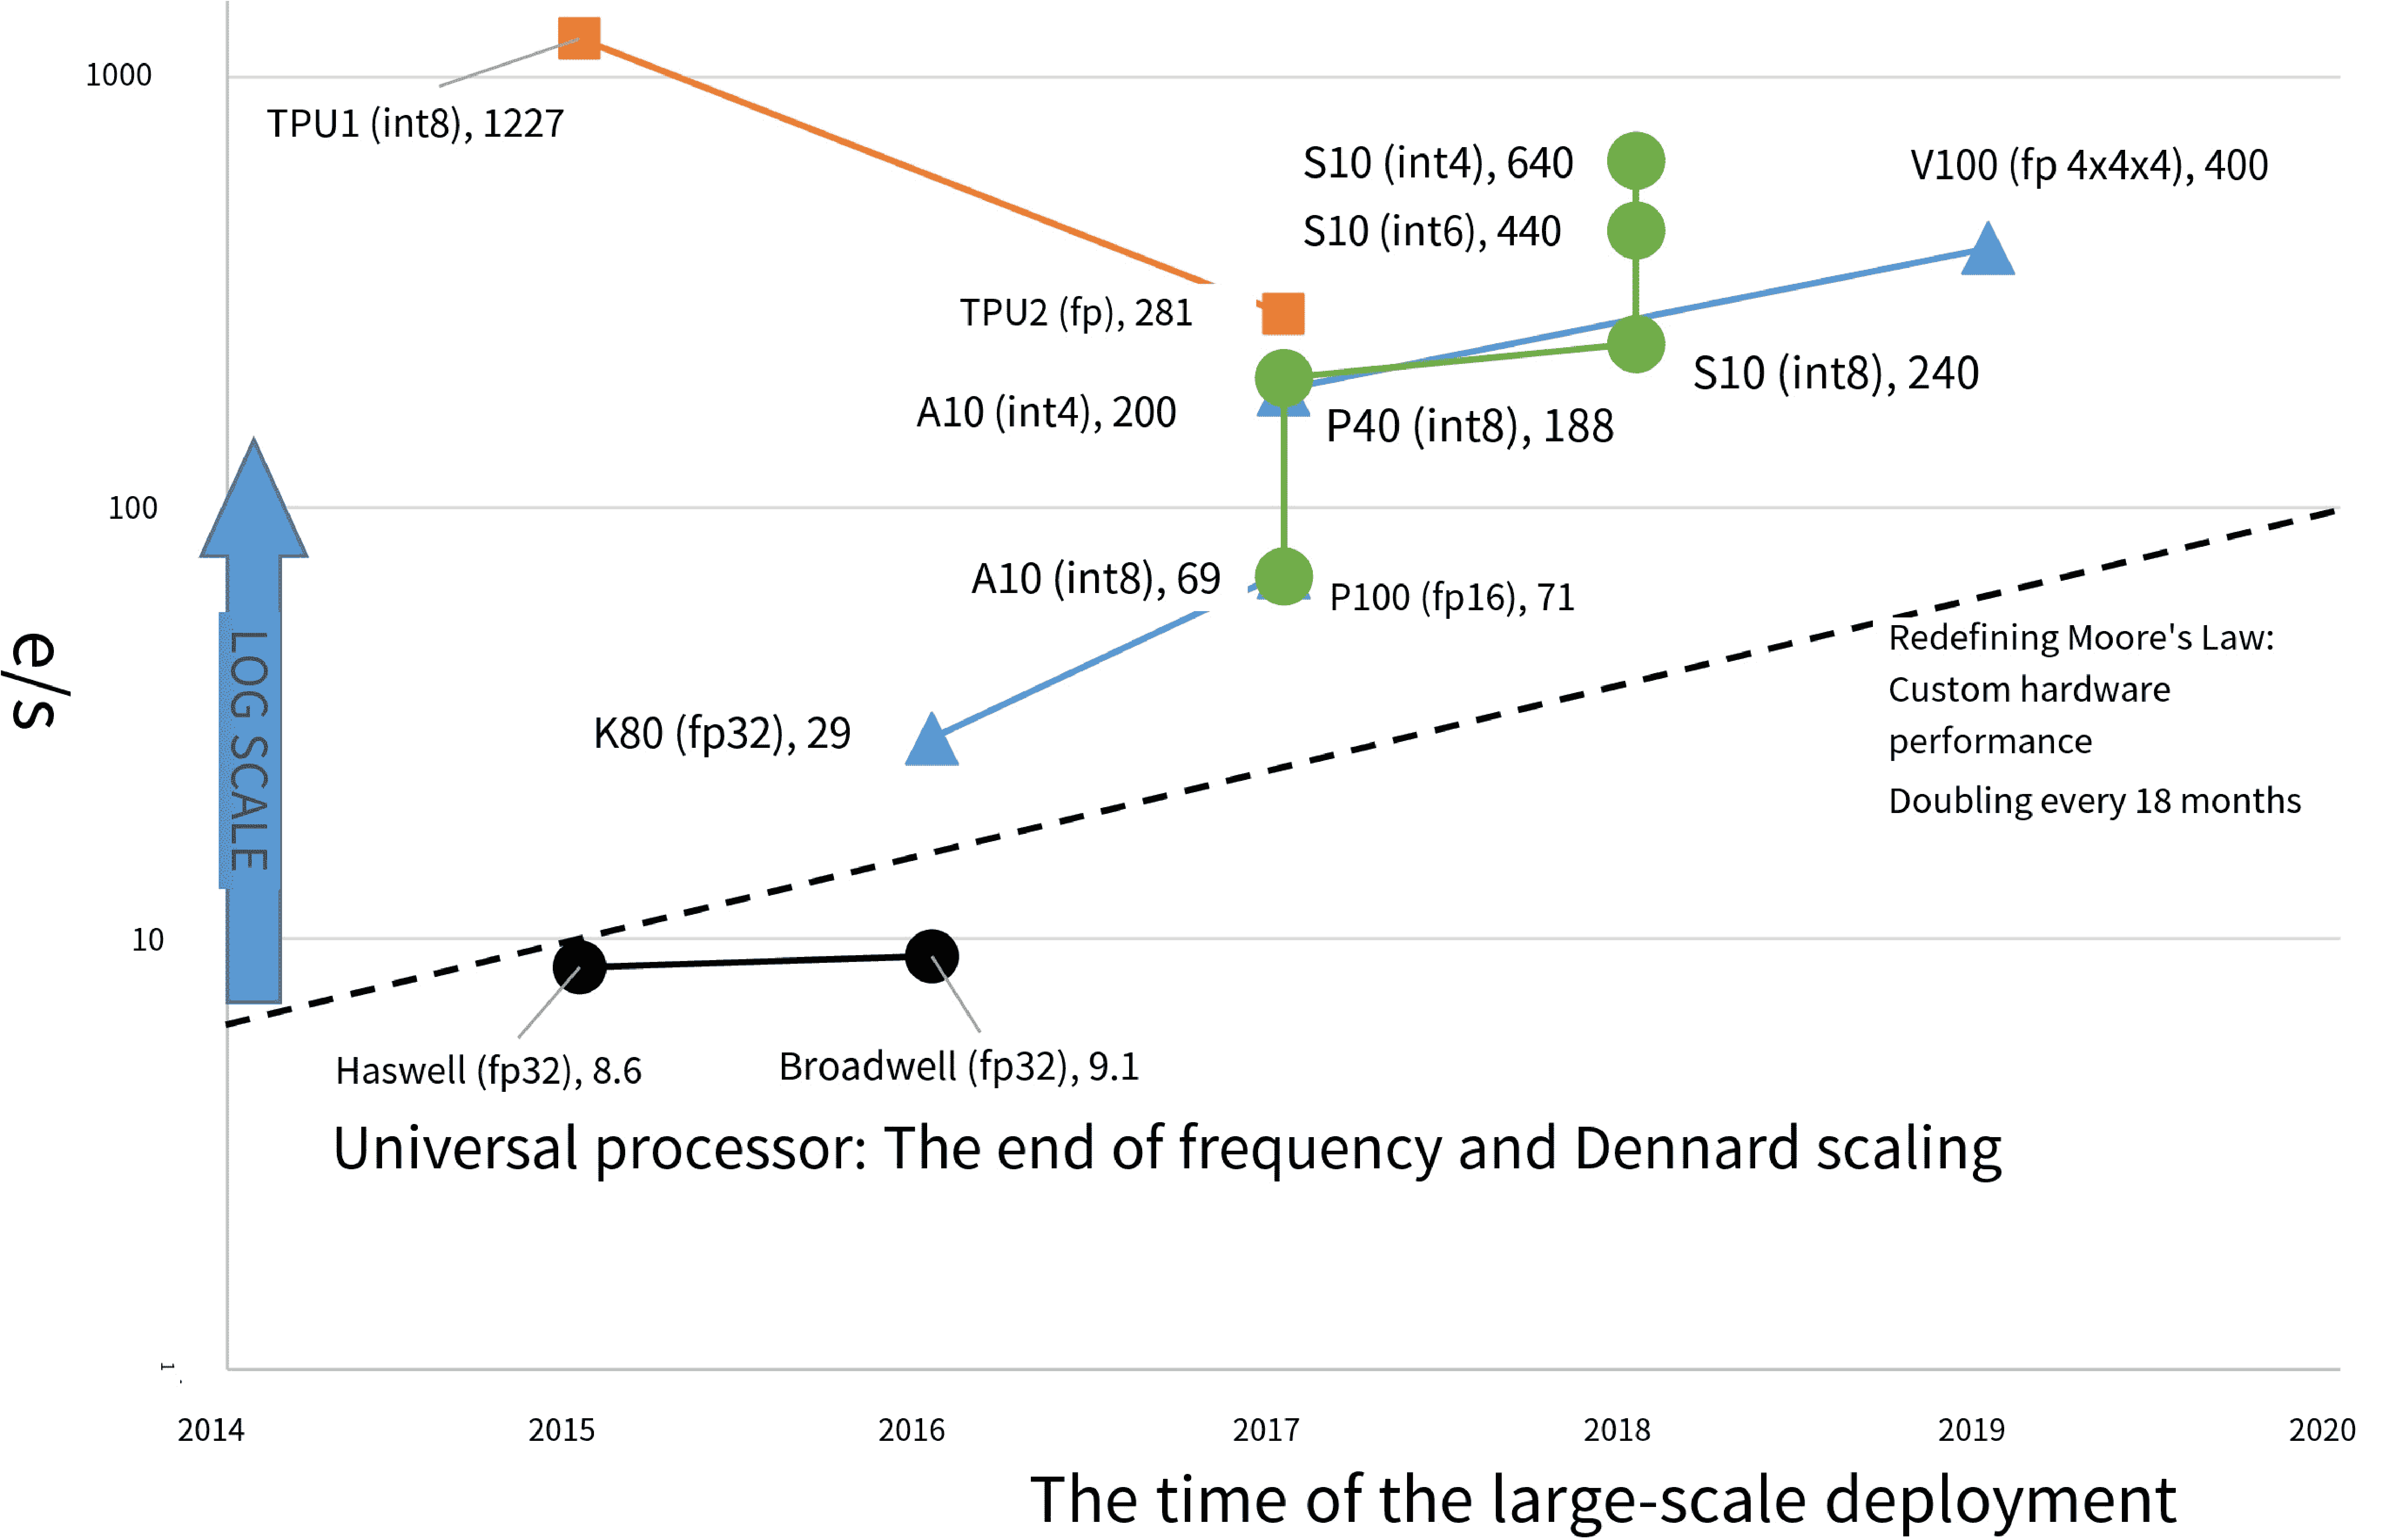
\includegraphics[width=0.8\textwidth]{figures/moores_law_redefined.pdf}
	\caption{通用处理器的频率和 Dennard 缩放逐渐终结,但定制化硬件重新定义并延续了摩尔定律。}
	\label{background:fig:moores_law_redefined}
\end{figure}

第二,操作系统,大量开销,数据中心税。

第三,软件开发,安迪比尔定律。

第四,数据中心层面:大部分物理服务器的使用率只有大约10\%到15\%,但是功耗却与使用率最高时相差无几。云为什么需要热迁移?


\iffalse

\subsection{芯片的发展}

计算机体系结构的进步是和半导体集成电路的发展分不开的。可以毫不夸张地说,计算机的发展是集成电路技术最大的推动力,也是最大的获益者。过去半个多世纪以来,集成电路一直大致保持着摩尔定律预测的速度发展,高度集成的芯片带来一次又一次计算机体系结构的革命,从巨型机(MainFrame)到个人电脑(Desktop),从服务器到云计算平台,从笔记本电脑到移动计算,集成电路使得各种形态的计算机快速地渗透到我们生活的方方面面。而另一方面,正是计算的需求,推动了中央处理器 (CPU),内存 (DRAM),图形加速器 (GPU) 以及高速网络芯片的发展。芯片技术和计算机体系结构相辅相成,共同推动了计算机系统软件和计算机应用的发展,使信息技术在短短的几十年中获得了如此重要的社会和经济地位。

目前信息科学技术依然处于一个高速发展的阶段,新的应用层出不穷:人工智能、物联网、虚拟现实、区块链,新兴的方向让人目不暇接,每一项技术都有无穷的潜力,可能推动人类社会进入全新的未来。而另一方面,基于半导体硅的CMOS集成电路芯片技术由于受到物理规律的限制,已经开始达到瓶颈。一方面芯片的线宽(Feature Size)在5纳米以下已经很难进一步缩小,而另一方面功耗和散热已经成为现代芯片技术难以绕过的难题。在这种情况下,计算机技术会何去何从?未来的计算机如何满足不断增长的计算能力的需求?

借助这篇短文,我们想探讨一下我们认为计算机系统在未来几年中发展的可能方向,尤其是集成电路技术如何与计算机体系结构继续相互推动,提高计算的速度和效率,满足不断增长的算力需求。目前学术界和工业界的共识是,科学家们看来不太可能找到短期内能代替CMOS的技术,计算机技术性能的提升在短期内必须主要依靠计算机体系结构的创新。在这篇短文里,我们着重探讨一下云计算平台的体系结构可能的发展趋势和方向。在可以预见的未来,云计算会是非常重要的计算平台,它会提供人类社会主要的算力,推动整个世界的数据处理能力。当然,移动计算、物联网以及其它“端”也是非常重要的发展方向,但限于篇幅,在这篇短文中我们就不详细探讨这些方面的发展。

\subsection{云计算平台的变革}

在21世纪初期,云计算的概念刚刚起步的时候,云计算的平台基本上就是一个普通的企业数据中心,只不过规模比较大而已。当时的云计算与传统意义上科学计算用的超算平台在硬件上有很大区别。科学计算用的超级计算机往往使用定制的芯片,定制的网络,不惜成本地追求最高的性能。而云平台的特点就是把普通的低端商用服务器规模化,用软件实现高容错、高可靠性,降低成本,提供高性能的服务。

随着云计算商业模式得到用户的认可,特别是公有云的概念被广泛接受,经过近二十年的发展,目前主要的云计算平台提供商已经取得了巨大的商业成功。云计算平台的规模已经大大扩张。业界领先的云平台已经拥有遍布世界各地数以百计的数据中心以及数以百万计的服务器。这对计算机的体系结构带来了非常多新的挑战。建设一个大规模的云计算平台需要巨大的投资,任何能够减少单机成本的创新都能带来极高回报;云计算需要大量电力维持运转,提高系统的效率,降低功耗是重要的指标;云计算平台的一个大卖点就是弹性和灵活的配置,如何提供弹性同时尽可能减少系统空闲是一个复杂的问题;云计算需要保证可靠性,需要易于管理,需要保护私有信息,这里有非常多的挑战都需要解决。

在计算机发展的早期,软硬件是由同一个公司团队开发的,许多黑科技在这个大环境下被发明创造出来,对后世产生了深远影响。随着计算机的发展,设计分工变得越来越细,CPU、内存、网络、操作系统等等计算机的组成部分逐渐由各个专业公司独立完成,这使得工程师们必须遵守现有的体系框架,跨界创新变得非常困难。虽然在某些专用领域(例如游戏机)设计师们还可能做系统全盘考虑,但在通用计算领域这几乎成了不可能的任务。


\subsection{可编程逻辑阵列FPGA 和专用集成电路 ASIC}

为了更好了解集成电路和计算机体系结构,需要在这里简单介绍一下两个重要的集成电路技术。

ASIC(Application Specific Integrated Circuit,专用集成电路)是为某些应用专门开发的集成电路芯片。ASIC开发门槛比较高,研发周期也比较长。在目前的技术水平下,中等复杂度的ASIC前期投入的一次性开发成本(NRE, Non-Recurring Engineering)会在数百万到一两千万美元左右,并且需要一两年的开发周期。

FPGA(Field Programmable Gate Array,可编程门阵列)是一种可以重新定制 (reconfigurable) 的集成电路元器件。直观上来说,FPGA就是一个可以用编程的方法重新组合的一大堆电子元器件。这些元器件包括逻辑门(如与,或,非门),寄存器 (Register),加法器,静态内存(SRAM)等等,用户可以定制它们之间的连接从而组成不同的电路。如今的FPGA除了基本元件,还加入了越来越多的DSP和硬核(hard IP),以提高乘法、浮点运算和访问外围设备的性能。FPGA的优点是技术比较成熟,开发门槛相对其它集成电路(如ASIC)较低,部署后依然可以修改,缺点是性能比专用芯片差。

FPGA传统上被广泛应用于原型设计,逻辑电路模拟,以及高端路由器等等的领域。最近几年FPGA开始被在数据中心中得到越来越广泛的应用。在数据中心中,FPGA主要被用在两个方面,一方面是用于部署后依然可能需要改变的应用上,比如网卡。由于公有云的网卡上经常需要调整或添加协议,需要经常对硬件重新编程。另一种应用是计算加速:对于一些特殊的计算,可以利用FPGA可以高度并行化的的特性加速。在数据中心中用FPGA加速应用的一个大概的规则是10,100,1000规则:应用需要可以被加速十倍以上,如果加速比太小就不值得做硬件的实现了;被加速的部分核心大约相当于100行以下的代码,更复杂的逻辑用硬件实现难度就会比较大;而计算在数据中心应该需要至少1000台左右的服务器,如果服务器数目远远小于1000台,可能就不值得开发硬件方案了。当然,这些数字都是非常粗略的估计,应该根据FPGA的部署情况,应用本身的价值,以及开发人员的实际情况做相应调整。

在过去,开发ASIC往往是专业硬件芯片公司才能做到的事情。但随着云计算平台规模的不断扩大,云计算系统公司也开始尝试针对自己的云独立设计专用芯片。
\fi

\section{数据中心硬件的发展趋势}
\label{background:sec:hardware}



现代计算机系统大致可以被划分成四个主要部分:计算系统(Compute)、内存系统(Memory)、存储系统(Storage)以及网络和互连系统(Networking and Interconnect)。


\subsection{计算系统}

计算系统是整个计算机的核心,通常是由中央处理器CPU和一些为特殊应用服务的加速器构成。从整个计算机体系结构的发展来看,计算系统上的创新可能是最受关注的一个领域了。

在过去,计算系统基本上就等同于CPU,而CPU上的创新是由Intel、IBM等少数几个大公司主导的。传统上计算力是计算机系统中相对比较富裕的资源。一方面得益于摩尔定律及CPU体系结构的进步,CPU的速度和效率得到了长足的进步;另一方面其它的子系统例如硬盘,内存和网络因为相对缓慢的进展而往往成为实际应用的瓶颈。这种情况在最近几年发生了很大改变:随着新的硬件如固态硬盘和超高速光通信网络的出现, I/O往往不再是瓶颈;而新的应用如深度学习和内存数据库等对算力有极大需求,传统的CPU已经越来越难以支撑这些应用。正因为如此,在计算系统上创新,也就是大家通常所说的异构系统成为近年来计算机体系结构研究的一个热点。

\subsubsection{深度学习加速器}

最近深度学习的热潮,使得计算加速成为一个热点。从大学到工业界,从初创企业到业界巨头,从传统的半导体公司到传统的应用软件开发商都在尝试设计专门针对深度学习应用的硬件加速器,为小到低功耗的IoT设备,大到整个数据中心设计解决方案。在云计算领域,谷歌作为利用集成电路ASIC加速深度学习的先行者,为此设计的专用张量处理器(TPU)目前已经发展到第3代,无论从技术创新,吸引眼球,还是商业运作方面都取得了极大的成功。微软利用FPGA做深度神经网络(DNN)加速,也已经在Azure云平台上线。

深度学习包括训练和推理两种场景。训练所需的内存大、运算复杂,大多部署在云数据中心,NVIDIA的GPU具有巨大的生态系统优势,仅有第三代TPU、Graphcore等少数深度学习加速器正在挑战其垄断地位。推理的应用场景则较为异构。移动计算场景下低功耗是最重要的需求,如寒武纪神经网络处理器以知识产权(IP)授权的形式集成进入华为麒麟970处理器;搜索推荐、自动驾驶和虚拟现实场景下,既需要毫秒甚至微秒级的低延迟,又需要较高的吞吐量。推理的多种场景下不仅有不同的性能指标,所需的神经网络运算也不尽相同。加速器除了支持循环神经网络、卷积、矩阵乘法、正则化等经典神经网络运算,还需要与场景相关的算法共同演进,利用稀疏化(sparsity)、量化(quantization)等技术在不降低精度的前提下提高算力,并支持动态控制流等新兴的神经网络结构。\textbf{cite 张宸的 paper}

\subsubsection{FPGA和可重构硬件}

用FPGA做计算加速在学术界已经被研究多年,在某些特定的领域也得到了一些应用。而将FPGA大规模部署在通用服务器上却是最近几年才开始取得的突破。很多公司都开始做一些这方面的尝试,特别是微软和百度在有效利用FPGA做云计算加速方面做了很多工作。例如微软在Azure云平台上已经全面部署了FPGA模块。FPGA在云平台上可以被广泛用于数据压缩、数据加密、图像处理、网络功能、大数据处理以及深度学习的加速。目前云计算一个探索的方向是将FPGA作为服务提供给第三方开发者。随着云端FPGA开发环境和开发工具的完善,越来越多的应用会利用FPGA的重构能力获得加速。

收购Altera后,Intel推出集成了FPGA的Xeon芯片,这将大大提高FPGA作为计算加速器的效率;而Xilinx则推出了全新的代号为Everest的可重构硬件构架,专门针对服务器的计算加速。这些技术必将对未来几年的云计算平台架构带来深远影响。除此之外,一些研究机构和初创企业开始再次尝试设计新一代粗粒度可重构硬件。粗粒度可重构硬件对于一些合适的应用可以兼顾FPGA可重构和ASIC高效率的优点,虽然过去的一些类似尝试最终没有取得商业成功,但云计算蓬勃发展的大环境很可能让这一技术焕发新的生命。\textbf{cite Intel Agilex 和 Xilinx ACAP}

\subsubsection{通用可编程加速器}

得益于深度学习的高速发展,传统的计算加速器比如NVIDIA的Tesla以及Intel的Xeon Phi近年来也在数据中心和云平台上取得了很大的成功。除了深度学习,这些加速器还可以被用于加速科学计算,数据库检索,机器学习,图像处理等许多不同领域的应用。这些可编程通用加速器主要是利用计算的并行性来获得比CPU更高的性能和效率。但是,目前已有的这些加速器主要是为高性能计算设计的,还没有公司专门为云计算平台的一些主流应用比如数据压缩,网络包处理,加密解密等等设计一个通用的加速器。这很可能是一个有一定潜力值得挖掘的新方向。

对加速器来说,一大挑战是普通的内存无法满足并行计算需要的数据吞吐带宽。利用3D封装技术实现的HBM(High Bandwidth Memory )最近开始被广泛应用在这些加速器中。随着集成电路工艺的改进,集成计算和内存于同一芯片的PIM(Processing In Memory)方法开始重新受到重视,在这个技术上的突破可能给可编程加速器带来性能的飞跃。

\subsubsection{通用处理器}

在可以预见的未来,云计算中的大部分代码,特别是不易并行的代码,仍将主要在CPU上执行。为了隐藏访存延迟,提高流水线利用率,CPU使用乱序和推测执行来动态调度指令的执行顺序。过去的推测执行在微体系结构方面的副作用导致了Spectre等安全漏洞,需要未来的CPU体系结构设计做出重大的改变。

乱序和推测执行受到指令窗口的限制,只能隐藏百纳秒级的延迟(基本对应于内存访问的延迟)。对于访问网络、存储、加速器等带来的微秒级延迟,还没有很好的解决方法。简单地增大乱序执行指令窗口是不现实的,而操作系统现有的线程切换机制开销过高。编程语言现有的协程(coroutine)机制一方面使编程变得复杂,另一方面在访问网络、存储、加速器等外设时仍然依赖开销较高的内存屏障。未来计算机体系结构的一大挑战是解决对程序员透明的微秒级细粒度并发。这需要CPU体系结构、编程语言和操作系统的协同设计。

通用处理器并不仅仅只存在于服务器的中央处理器。加速器、硬盘、网卡等设备上一般也有用于控制和通信的处理器。此类处理器往往需要根据领域需求定制,而使用MIPS或ARM需要不菲的授权费。最近,加州大学伯克利分校提出了RISC-V,一种开放的指令集架构(ISA),以缩短定制化处理器架构的周期和成本。RISC-V以及其相对应的软件生态的出现和完善使得Intel,ARM之外的公司和个人也可以在CPU体系结构上创新,而不用被编译器,操作系统,及上层的应用生态限制。RISC-V这一开放指令集架构的运动必然会对未来CPU的生态产生非常大的影响。很多公司会有机会完全抛弃Intel和ARM另起炉灶,为自己的应用设计和生产自己的CPU。让我们拭目以待。

\subsubsection{软件的挑战}

对所有提高计算系统效率和性能的技术来说,可编程性永远是一个无法绕过的坎。近年来,硬件的高层次综合技术和软件并行编程技术都有了很大的进展,这降低了利用新的计算资源的门槛。尽管如此,如何方便而有效地利用这些非传统的计算资源依然是一个长期的难题,需要大量的持续投入。

不同于PC时代分工明确、由各个公司分别掌控的标准化模块,云计算中从硬件到软件全栈优化和定制化的需求是开源生态系统近十年来蓬勃发展的主要驱动力之一。未来的异构计算软件框架也将形成开放的软硬件接口标准和开源生态系统。

\subsection{内存系统}

内存系统用来存放程序运行时的代码和数据。目前几乎所有的计算机系统上,内存系统都是由少量基于静态内存(SRAM)的缓存(Cache)和大量的动态内存(DRAM)组成的。除了极少数为科学计算或超大型数据库设计的高性能计算机外,绝大部分计算机上的内存只能被本地同一主板上的一颗到几颗CPU芯片访问。在过去的半个世纪以来,内存系统的主要特性都一直没有什么变化,非常令人振奋的是,最近几年内出现的几项新技术可能会改变这一现状。

\subsubsection{高速非易失性内存(Non Volatile Memory,NVM)}

目前被广泛使用的动态内存(DRAM)制造工艺已经接近物理极限,价格一直居高不下,另外,DRAM需要不断刷新来保持数据,功耗较高。长期以来科学家们一直在寻找能够代替DRAM的存储器件。通过科学家们多年以来不懈努力,一直声称有希望取代DRAM的高速非易失性内存目前看来终于快要进入实际应用阶段了。相比传统的NAND Flash,新一代的高速非易失性内存存取速度要快得多。虽然它们短期内还不能完全取代DRAM,但至少希望能够在不久的将来会代替一部分普通内存。目前看来,Intel和Micron合作的3D XPoint技术 \cite{3d-xpoint} 会是最快进入市场的非易失性内存,另外一些基于忆阻器件(ReRAM) \cite{akinaga2010resistive} 和磁阻器件(MRAM) \cite{tehrani1999progress} 的非易失性内存可能会紧随其后进入市场,学术界也在积极研究相变内存(PCM) \cite{raoux2008phase,lee2010phase} 和 STTRAM \cite{kultursay2013evaluating,apalkov2013spin} 等非易失性内存技术。

非易失性内存相比DRAM有价格低,容量大,功耗小,断电可以保持数据的优点,但同时又有存取速度慢,写入周期有限等等限制。如何有效地利用非易失性内存目前是一个重要研究方向。
目前,大多数工作把非易失性内存当作介于动态内存和闪存持久化存储之间的存储层级,即所谓的 ``慢速内存'',形成两层的异构主存体系结构 \cite{dulloor2016data,agarwal2017thermostat}。
在应用程序的使用接口方面,大多数工作把非易失性内存抽象成块设备 \cite{bailey2011operating,huang2014nvram,kim2016nvwal,mogul2009operating,nanavati2017decibel,hu2017log} 或文件系统 \cite{condit2009better,yang2015nv,xu2016nova},并支持标准的 POSIX 接口。
为了降低操作系统软件存储协议栈开销,NVTree \cite{yang2015nv}、NVWal \cite{kim2016nvwal}、NOVA \cite{xu2016nova}、Decibel \cite{nanavati2017decibel}、LSNVMM \cite{hu2017log} 等工作旨在高效管理存储在非易失主存中的数据。
PASTE \cite{honda2018paste} 提出了存储和网络协议栈的协同处理。
从体系结构的角度,为了消除应用程序访问非易失性内存的额外软件开销,AMD 等 CPU 厂商正在通过改进内存控制器,把非易失性内存映射到 CPU 的内存地址空间,从而应用程序可以像访问动态内存那样访问非易失性内存。


\subsubsection{内存解聚(Memory Disaggregation)}

传统的服务器上的CPU、内存、存储等资源聚合在一起成为独立的单元,一台服务器需要通过网络API访问远程的资源,使用上非常不便和低效。目前一个计算机体系结构研究的热点是资源解聚,也就是让资源可以不受服务器物理边界的限制被透明地远程访问。内存解聚指的是计算机的计算系统(CPU、GPU等)可以自由而透明地高效共享远程计算机的内存,这样可以大大增加内存的利用率,降低云计算平台的成本。

要想实现这一目标,计算机系统的软硬件都需要做很大的改变。从硬件上来看,如何能让远程访问满足内存所需的带宽和延迟要求是一个巨大挑战。幸运的是,利用内存访问的局部性,如果一部分热数据仍在本地,剩余的数据通过远程访问,则远程内存的带宽和延迟要求能比本地内存大大降低。加州大学伯克利分校的研究指出,要把内存解聚后的系统性能与全部使用本地内存的差距控制在5\%以内,带宽需要达到40 Gbps,端到端往返延迟需要不超过3~5微秒。现代数据中心的带宽已能满足大多数应用的需求,但延迟仍有一个数量级的差距。

从系统软件上来说,如何有效共享远程的内存,让应用克服远程内存访问的延迟和带宽限制也有很多问题需要解决。与传统的swap不同,把一块内存放在远程会减少对应远程机器的本地内存,因此一块内存放在本地还是远程、放在远程的哪台机器上,需要根据集群全局的信息来决策。另外,远程内存的延迟远大于本地内存,当等待远程内存时,如果不希望CPU核闲置,就需要调度其他任务。前面“通用处理器”一节已经谈到,这种微秒级的延迟隐藏仍是一个没有很好解决的问题。

\subsubsection{HBM(High Bandwidth Memory )}

HBM使用2.5D集成电路封装技术,将内存和逻辑芯片封装在同一硅片衬底中,从而提供更高的带宽。前面已经提到HBM已经开始被用到计算加速器上,但目前这一技术还没有用在通用的计算CPU上。一方面普通外置DRAM已经可以满足通用CPU带宽的需求,不需要高成本的HBM,另一方面现代应用通常需要很大的内存容量,目前的HBM还无法满足。但是从系统整体设计的角度来看,计算加速器独占高速内存是不正确的设计。CPU应该和加速器共享高速内存,这样不仅能够更充分地利用HBM,同时CPU和加速器之间的协同也更加简单高效。但是目前由于CPU和加速器是由不同公司设计制造的,所以只能采用一个权宜的设计。如果单个公司控制整个系统的设计,可能结果就不一样了。在微软的XBOX One X 中,CPU就是和GPU共享高速的GDDR5的,而AMD的APU也一直在推动CPU和GPU共享内存。随着计算加速的普及,在以后的云平台中CPU可能会与加速芯片共享HBM。从CPU角度看HBM就是一块高速内存,而普通DRAM就会成为一个容量的扩展,变成内存层次(Memory Hierarchy)中的另外一层。

\subsubsection{软件的挑战}

传统的内存层次(Memory Hierarchy)通常有三层。cache是透明的,用户的程序一般不需要直接操作;而可以按照字节寻址的DRAM的性能是统一的,这是应用程序需要控制的内存区域;对用户完全透明的虚拟内存(Page Swap)虽然理论上非常优美,但由于内存与磁盘之间的延迟相差多个数量级,实际使用中很小比例的内存不命中就会极大影响应用的性能,所以一般是万不得已的最后选择。新一代的内存系统势必需要在传统的内存层次中再增加一个层次。用户程序是需要显式调用专用的API去存取这片内存,还是应该对应用透明?这个层次的内存应该如何能够被高效使用目前还没有定论。

\subsection{存储系统}

存储系统过去主要是由基于磁介质的硬盘和磁带组成,近年来基于NAND  Flash的固态硬盘被广泛应用于数据中心,而磁带已经开始淡出历史舞台。与内存系统不同,存储系统主要用来存放需要长期保存的数据。

\subsubsection{SCM(Storage Class Memory)}

SCM实际上是上一小节中讨论过的高速非易失性内存的另一种描述方式。在传统的计算机体系结构中,基于DRAM的内存和基于硬盘的存储是完全不同的两个系统,它们分别由操作系统中的内存管理系统和文件系统分别管理,基本上井水不犯河水。可是随着技术的发展,高速非易失性内存有潜力成为可以同时代替内存以及硬盘的一种器件,这时文件系统和内存系统的边界就开始模糊起来了。将高速非易失性内存用文件系统管理起来,利用它的非易失特性储存需要长期保存的数据就是SCM。SCM的出现对存储系统提出了新的挑战,如何有效地利用SCM高带宽、低延迟、可字节寻址的特性加速应用程序是一个需要解决的问题。

首先,机械硬盘和基于NAND Flash的固态硬盘是以“块”为基本单位来读写的,从而随机读写的性能远低于连续读写。SCM可以按照字节寻址和读写,随机与连续读写的性能差距较小,从而降低了应用对数据排布的要求。很多应用可以把SCM文件映射到内存后直接访问,省去在文件存储格式和内存数据结构间来回转换的开销。

其次,传统系统为了在断电或系统崩溃后能够恢复,往往需要日志和快照技术来把一致的内存状态显式写入存储系统。利用SCM的非易失特性,把DRAM作为SCM的写通(write-through)缓存,应用就可以直接操作其上的数据结构而无需额外的日志和快照。

\subsubsection{存储解聚(Storage Disaggregation)}

类似于内存解聚,存储系统同样可以通过解聚来提高利用效率和性能。微软研究院将存储系统的解聚分为四个层次。一是配置解聚,即标准的机柜(rack)离线配置成存储阵列或计算阵列。二是故障解聚,即计算节点发生故障时把其硬盘分配给新的计算节点,无需搬运数据即可恢复服务。三是动态弹性解聚,即根据计算和存储的需求比例动态调整每块硬盘属于哪个服务器。前三个层次中,每块硬盘在每个时刻只属于一个服务器。四是完全解聚,即每个服务器都可以访问任意设备上的任意文件,还可以在IO操作的细粒度上做负载均衡,当然这对IO控制器的负载要求较高。

与内存系统相比,由于存储系统本身的带宽较低、延迟较高,存储系统解聚面临的挑战相对要小一些,一个主要的问题是如何能在资源共享的情况下能够减少用户之间的相互干扰(即性能隔离)以及保证服务的质量(QoS)。

\subsubsection{开放通道(Open Channel)SSD}

如今服务器里的固态硬盘大多基于NAND Flash。NAND Flash的每个闪存块需要先擦除再写入,每次擦除会造成一定的磨损,多次写入有的闪存块就会损坏;闪存块读取次数多了、闲置时间长了,上面的数据也会流失。因此,固态硬盘中的闪存转换层(FTL)除了从逻辑地址到物理地址的映射,还需要做一系列的处理。这些处理需要预留一部分存储空间、占用带宽来做垃圾回收和冗余,还会导致写操作时搬运周围数据带来额外开销。如果考虑到应用的读写特性和数据中心的外部冗余,FTL的很多操作在云计算数据中心中是不必要的。因此,开放通道(Open Channel)SSD在数据中心开始流行,应用直接管理闪存阵列,FTL的功能与应用程序就可以协同设计以提升性能。

\subsubsection{软件的挑战}

传统存储系统操作通常需要操作系统的参与。过去,硬盘的速度较慢,操作系统的开销往往可以忽略不计。随着高性能存储介质的出现,应用程序与操作系统之间的上下文切换以及操作系统内文件系统和块设备层的开销逐渐成为性能瓶颈。为此,Intel 提出的SPDK提供了绕过内核的应用直接访问存储接口。然而,当多个应用需要共享文件系统时,应用间的权限管理、并发控制和QoS仍是有待研究的问题。

\subsection{网络和互连系统}

网络(Networking)系统通常指用来连接多个计算机使它们之间能够相互通信的系统,而互连(Interconnect)一般指计算机内部的部件之间的连接。通常情况下这两种连接是有着巨大差别的,属于两个完全不同的学术领域。一个典型的网络,比如数据中心网络,通常需要跨越较长距离、对延迟不敏感的传输,需要多层路由和交换来连接为数众多的节点,丢包是靠软件检测和恢复的,且一个组件的故障一般不会影响网络其他部分的正常运行;而一个典型的互连,比如连接内存和CPU的总线,位宽和带宽会比较大,延迟很低,丢包会由硬件检测和恢复,但一个组件的故障可能导致整个系统的崩溃。

在互联网发展的早期,以搜索引擎为代表的应用比较容易并行化,因此对网络通信的需求不是很高,数据中心通常使用现成(off-the-shelf)的服务器通过以太网互连。最近,大数据处理、分布式机器学习、内存和存储等资源的解聚需要数据中心主机间低延迟、高带宽的通信。GPU和深度学习处理器为了做分布式训练和推理,也需要建立可扩放(scalable)的互连。由于高速可扩放通信需求的推动,有一个很有意思的趋势就是融合传统的网络和元器件之间的互连。比如常见的PCI-Express,开始设计的时候是为了连接单一机器内的不同部件,但是现在,PCI-E也被设计为可以交换的一个协议;而以太网的开始时是设计为连接局域网内计算机的一个网络,而如今一些器件间的连接也开始使用以太网的连接方式。

\subsubsection{低延迟无丢包的可扩放互连}

理想的网络和互连需要既能扩放到数据中心内数以百万计的设备和组件,又有低延迟、高带宽、无丢包的特性,还能容忍部分组件的故障甚至恶意攻击。为此,网络和互连的设计者一方面可以从很多历史设计中吸取经验,如超级计算机、片上网络、核心路由器的线卡间互连、电路交换网络、时分复用网络等;另一方面可以利用新的物理层技术,如光交换芯片、激光通信和60G无线网络等。

数据中心内从发送端网卡到接收端网卡的网络延迟主要包括光纤上的传播延迟、交换机的处理延迟和交换机内的排队延迟,其中排队延迟占了主要部分。为了降低排队延迟,数据中心交换机普遍使用ECN、RED等机制来把拥塞情况反馈给发送端,但这个反馈延迟往往较长,且不能消除来自不同发送端的数据包恰好撞在一起导致的偶发排队。为此,近期一系列研究在重新思考现有的拥塞控制算法,交换机也需要更灵活的动态控制来尽可能降低队列长度、保证服务质量。例如,微软 Azure 云 \cite{guo2016rdma}、阿里云 \cite{aliyun-rdma} 和华为云 \cite{huawei-lossless} 建成了大规模数据中心 RDMA 网络,构建了低延迟、高吞吐量、无丢包的数据中心网络,为大数据处理和大规模机器学习提供了高性能网络互连。

更深层的问题是Internet的端到端原则简化了设计、提高了鲁棒性,但也缩小了很多全局优化的空间。在端到端原则的指导下,很多数据中心的网络交换机和主机网络协议栈是由不同部门独立运维的,这也增加了协同设计的沟通成本。在网络和互连融合的未来数据中心,端到端原则在多大的范围内适用是一个值得思考的问题。

随着主机内异构计算和存储设备数量的增加,CPU的PCIe接口数量不足,PCIe交换机开始被引入主机;由于PCIe的带宽不能满足需求,GPU之间采用NVLink互连,随着互连GPU数量的增加也出现了交换机。为了解决异构计算和内存设备之间的互连,工业界成立了CCIX、Gen-Z和OpenCAPI三个开放标准组织,其中OpenCAPI最先商业化,Gen-Z的应用范围最广。数据中心网络的发展历史表明,异构计算设备之间的可扩放互连必须考虑容错性和安全性。

\subsubsection{可编程交换机}

可编程交换机是由需求和硬件两方面的趋势所驱动的。从需求方面来讲,网络的自动运维(self-driving network)变得越来越重要。要实现自动化的网络故障检测、诊断和恢复,就必须在网络中加入智能,而不能把网络看成一个黑盒子。为此,交换机中需要加入可编程的抓包和统计功能。不仅如此,利用交换机的高速数据包处理能力,可以加速分布式系统中的缓存、聚合、同步、事务处理等,而低延迟无丢包网络也需要可编程交换机硬件的支持。很多人认为在交换机中增加可编程性会增加芯片面积和功耗,其实并不尽然。交换机芯片中约有30\%的面积用于串行IO通信,50\%的面积用于存储查找表和数据包缓冲的内存,只有20\%的面积用于数据包处理逻辑。随着交换机的带宽不断增长,芯片面积也在增加,此时用于数据包处理的20\%面积就有空闲,可以放入更多逻辑。

可编程交换机按照可编程性从低到高,可分为三个层次。一是符合OpenFlow标准的交换机,数据包处理逻辑是一条由若干个匹配-执行表串接而成的流水线,但每个表的匹配和执行都有一定的限制;二是符合P4标准的交换机,在流水线结构的基础上,每个表项的匹配规则、所执行的操作和数据包头的解析规则都可以定制;三是网络处理器,即使用为网络处理特别设计的众核CPU处理每个数据包,可以达到最大的灵活性,但单条网络连接的吞吐量受限于CPU频率。事实上,固定功能流水线、通用可编程流水线和网络处理器并不是泾渭分明的,在数据中心交换机中已经可以看到逐渐融合的趋势,例如采用交叉开关或片上网络来灵活互连各个数据包处理模块和片上内存。

为了简化交换机运维和管理,微软发起了SONiC白盒交换机开源项目。首先,定义了一组交换机芯片API,交换机的硬件和软件就可以独立演进而无需担心兼容性问题。其次,设计了基于容器的模块化交换机软件架构,通过把持久状态独立于容器存储,实现了细粒度的故障恢复和零服务中断时间的在线升级。最后,提供了监控和诊断能力,以支持网络的自动运维。

\subsubsection{可编程网卡}

传统以太网网卡的功能相对简单,网络协议栈在操作系统内核里实现,软件中间件又给应用程序提供了RPC、消息队列等更高层的抽象。在云计算场景下,还需要虚拟交换机软件来实现网络虚拟化和防火墙等网络功能。因此,数据中心网络的端到端往返延迟平均情况就高达上百微秒,极端情况甚至可达毫秒级,远远不能满足低延迟分布式计算的需求。其中,软件的延迟占了主要部分。高性能计算中常用的Infiniband网络把大部分网络协议栈实现在网卡里,可以实现端到端微秒级的延迟,因此其中的远程直接内存访问(RDMA)技术开始在数据中心中流行。为了与现有数据中心网络兼容,数据中心的RDMA网卡通常使用以太网和UDP/IP,再在其上封装RDMA可靠传输协议。但云计算数据中心的RDMA部署比高性能计算复杂很多:首先,数据中心的规模大于高性能计算集群;共享同一物理主机的虚拟机需要隔离和QoS,也就是网络虚拟化;虚拟机需要热迁移和故障恢复能力;另外,数据中心应用种类繁多、通信模式复杂,需要兼容性和高层抽象。
为解决网络虚拟化需求,很多云数据中心大规模部署了可编程网卡,以把软件中的网络功能卸载到网卡硬件。可编程网卡是本文讨论的重点,我们将在第 \ref{smartnic-architecture} 节中详细讨论。

\subsubsection{设备间的智能互连}

传统计算机架构中CPU是中心,所有外设之间的通信都要通过CPU。近年来,CPU性能的提升放缓了,GPU、FPGA、TPU等异构计算设备和网络、存储的性能却突飞猛进,因此CPU日渐成为瓶颈。网卡、GPU、NVMe SSD等设备迫切需要绕过CPU的直接互连互通,因此出现了NVLink这样的专用互连,以及GPU-Direct和NVMe Over Fabrics等直接访问远程主机设备的技术。Broadcom也推出了可以通过以太网连接的PCIe交换机,使PCIe跨越了主机的边界。

然而,现有的技术大多只能互连一定范围内的特定设备。为了让数据中心内的所有异构计算和存储设备都能跨越主机的边界直接互连,微软研究院提出了Terminus项目,将互连(Fabric)作为一台服务器的控制中心,Fabric 控制器之间通过数据中心网络互连。通过在Fabric中加入智能,可以在不同厂商的计算和存储设备之间做 “翻译”,使它们在统一的命名空间中能够互相通信;Terminus也可以实现不同设备间的访问控制、通信性能隔离和服务质量保证;另外,Terminus可以支持资源虚拟化,既可以把多个物理的计算或存储资源虚拟成一个对用户透明的逻辑资源,又可以把一个物理资源虚拟成多个逻辑资源来实现多个用户间的资源共享;最后,Terminus 上的FPGA和可编程的数据中心网络可以在数据传输过程中进行一些处理,加速一系列的计算任务。Terminus项目目前使用FPGA作为原型,在未来也可以实现为智能的PCIe交换机。它与智能网卡、智能交换机一道,构建起数据中心的智能互连(Intelligent Fabric)。此时的数据中心可以被真正看作一台大型计算机,CPU、GPU等异构的计算资源和SSD、SCM等存储资源通过智能互连相连接,把分布式系统的通信、调度、容错等机制隐藏在统一的抽象之下,给用户提供取之不尽的计算资源和前所未有的编程便利。


\subsubsection{软件的挑战}

与存储系统类似,网络系统传统上被视为慢速的外设,再加上交换机排队、网络协议栈和中间件的高延迟,目前很多分布式系统并没有充分利用数据中心网络的高带宽和低延迟。近年来,绕过内核访问网络的用户态协议栈如雨后春笋般出现,\textbf{改进多核调度的工作(如 Adam Belay OSDI 18), FIXME}。我们相信,打破主机边界的软硬件协同设计将是网络和互连的趋势。

\subsection{全栈创新}

把整个世界看作一台大型计算机是微软CEO萨蒂亚·纳德拉的愿景,也是很多系统研究者的梦想。云计算的成功使数据中心吸纳了人类世界大部分的计算和存储,而数据中心可以看作是由计算、内存、存储和网络及互连四部分组成的一台大型计算机。系统就是从全局的角度考虑各种软硬件组件如何高效而可靠地协同工作,以及给用户提供怎样的抽象。从大型机、PC、传统数据中心到云计算数据中心,每个时代的系统结构都随着应用的需求而变化。

在目前机架服务器构成的数据中心中,一台标准(非深度学习)机架服务器的热设计功耗(TDP)为 300 至 500 瓦,按照目前的芯片制程,能够支持约 1000 平方毫米的芯片面积。
从理论上说,我们可以量化计算各种应用负载在不同体系结构上的功耗性能比,进而在不同的芯片间分配这 1000 平方毫米,求得每种体系结构芯片的最佳面积。
然而,这种方法并不现实,因为在设计服务器系统时,必须考虑多方面的限制。
例如通用处理器 CPU 上需要运行客户基于 x86 的应用,而 Intel 和 AMD 可选择的 CPU 型号是有限的。
再如,一款神经网络处理加速芯片(NPU)从设计到量产至少需要两年时间,我们很难为了设计一款新服务器机型等待如此长的时间,而只能在市场上已经或即将量产的加速芯片中做出选择。
此外,芯片之间的互连也需要遵循一定的标准,如 PCIe、CCIX 等,一种新的互连标准尽管设计起来不难,但需要较长的时间来寻求芯片厂商的支持。很多时候互连标准的选择不是纯技术的问题。
最后,服务器机箱(chassis)的设计涉及到散热等问题,需要积累经验,而在已有机箱布局和散热设计的限制下,芯片和板卡的数量甚至功耗就受到一定的约束。
因为芯片、互连和服务器机箱的可选方案是离散的,我们需要对各种组合进行全面的比较和分析,并得出最佳的方案。
当然,随着应用负载的变化,云服务商和板卡、芯片厂商也会调整芯片的体系结构设计和互连标准,逐渐向理论上最优的服务器组件结构靠拢。

如果我们可以抛开由机架服务器构建大型数据中心的现有模式,就有更多全栈创新的可能性。

\subsubsection{深度学习加速器集群}

深度学习和传统机器学习……TPU……

\subsubsection{机架级计算(Rack Level Computing)}

目前的数据中心的基本组件是由固定数量的CPU、GPU、内存、存储等资源构成的服务器。一方面,一台服务器中能容纳的硬件资源数量较少,只能同时运行少量任务,每个任务对不同种类资源的需求不均衡,这就会导致服务器中有的资源短缺,有的资源闲置。另一方面,CPU、内存和存储技术在成本、性能和功耗方面的演进趋势大不相同,要增加一种新硬件,往往需要重新设计服务器主板和机箱,需要较高的成本和较长的上市周期。前文提到的内存解聚和存储解聚通过访问远程内存和存储,只能解决第一个问题,可以认为是资源解聚的一个过渡期方案。完全的资源解聚需要重新思考以服务器为中心的数据中心设计。目前的趋势是把数据中心的基本组件从服务器变成机柜(rack)。机柜由若干个资源刀片(resource blade)和高速互连组成,每个资源刀片是一个装满同一种硬件资源的物理容器。在目前的数据中心里,存储阵列就像是这样的资源刀片。这样,CPU、GPU、内存、存储等不同种类的计算资源分别装在不同的资源刀片里,可以独立演进。当然,GPU和CPU仍然有本地DRAM或HBM内存作为缓存,而内存刀片则由高达数TB的DRAM或NVM组成,可以存储相对冷的数据。

\subsubsection{边缘数据中心}

目前的云计算数据中心大多规模庞大,部署在电力成本低、网络条件好的地区。用户访问最近的数据中心,也往往需要数毫秒到数十毫秒的延迟,带宽也受到一定限制。随着物联网、机器视觉、虚拟现实、自动驾驶等技术的发展,终端数据产生了越来越多需要实时处理的数据,此时把数据全部上传到云端在带宽和延迟上都是不可行的。为此,边缘数据中心开始兴起,把云计算搬到距离用户更近的位置。一方面,边缘数据中心可以降低用户访问互联网服务的延迟,例如现在的内容分发网络(CDN)服务。另一方面,边缘数据中心可以把终端设备上的部分计算和存储卸载到云端,降低移动设备的功耗、体积和成本,方便应用的部署和更新。

边缘数据中心将给云计算带来前所未有的挑战。首先,数据中心的数量将非常庞大。目前一家云服务约有几十个数据中心,开发者可以人工决定把服务部署在哪些数据中心。但对深入到每个城市、小区、楼宇的边缘数据中心,手工选址和部署就完全不现实了,因此需要全自动的方案。一个服务的数据被拆分到星罗棋布的数据中心,如何维护数据的一致性又不损失性能也是一个难题。其次,规模不大的边缘数据中心需要支持数量繁多的应用,这就需要细粒度的资源共享。目前云计算的粒度已经越来越细,从虚拟机到容器(container)再到函数(serverless function),边缘数据中心将延续这一趋势。


\section{可编程网卡的架构}
\label{smartnic-architecture}

\textbf{现在的 SmartNIC 不是单个芯片,而是片上系统(SoC)。例如 Mellanox ConnectX-5 firmware。根据数据面来区分架构分类。}

\subsection{专用芯片(ASIC)}
\label{smartnic-asic}


ASIC(Application Specific Integrated Circuit,专用集成电路)是为某些应用专门开发的集成电路芯片。ASIC开发门槛比较高,研发周期也比较长。在目前的技术水平下,中等复杂度的ASIC前期投入的一次性开发成本(NRE, Non-Recurring Engineering)会在数百万到一两千万美元左右,并且需要一两年的开发周期。


在过去,开发ASIC往往是专业硬件芯片公司才能做到的事情。但随着云计算平台规模的不断扩大,云计算系统公司也开始尝试针对自己的云独立设计专用芯片。

TCP Offload Engines

Mellanox ConnectX-5: programmable match-action tables for OVS, QoS, virtual switch, RDMA / RoCE...

Programmable, but not Turing complete. Not flexible.

学术界提出的可编程网卡架构:FlexNIC, Emu, SENIC, sNICh, Uno, Your Programmable NIC Should be a Programmable Switch,HotNets'18


传统上,微软与网络ASIC供应商(如英特尔,Mellanox,Broadcom等)合作,为Windows中的主机网络实现卸载 - 例如,在20世纪90年代的TCP校验和分段卸载[9],接收端扩展(RSS)[ 10]和虚拟机器队列(VMQ)[11]用于2000年代的多核可扩展性,以及最近无状态卸载用于Azure的虚拟网络方案的NVGRE和VxLAN封装在2010年[12]。事实上,GFT最初设计为由ASIC供应商实施,与SR-IOV一起作为精确匹配行动表,我们在业界广泛分享早期设计理念,看看供应商是否能满足我们的要求。随着时间的推移,我们对这种方法的热情逐渐降低,因为没有出现能够满足第3节中规定的所有设计目标和约束的设计。

SmartNIC供应商面临的一个主要问题是SR-IOV是一个全有或全无卸载的例子。如果在SmartNIC中无法成功处理任何所需的SDN功能,则SDN堆栈必须恢复为通过基于软件的SDN堆栈发送回流,几乎丧失了SR-IOV卸载的所有性能优势。



用于SDN处理的定制ASIC设计提供了最高的性能潜力。然而,随着时间的推移,它们缺乏可编程性和适应性。特别是,需求规格与硅的到货之间的长时间跨度大约为1  -  2年,并且在这个范围内需求持续变化,使得新的硅已经落后于软件要求。 ASIC设计必须继续为服务器的5年生命周期提供所有功能(以我们的规模改造大多数服务器是不可行的)。全有或全无卸载意味着今天制定的ASIC设计规范必须满足未来7年的所有SDN要求。

ASIC供应商通常会添加嵌入式CPU内核来处理新功能。与其他NIC处理硬件相比,这些内核可能很快成为性能瓶颈。此外,随着新功能的增加,这些内核可能会随着时间的推移而增加处理负担,从而加剧了性能瓶颈。这些内核通常也通过NIC的固件更新进行编程,由ASIC供应商处理并减慢新功能的部署。


\subsection{网络处理器(NP)}
\label{smartnic-np}

Queues + Flow Processing cores + accelerator ASIC + controller core

Mellanox NP-5, Netronome NFP-32xx, Cavium OCTEON

在服务质量(QoS)方面,硬件调度器比软件调度器不仅 \cite{kaffes2019shinjuku,ousterhout2019shenango}


\subsection{通用处理器(SoC)}
\label{smartnic-soc}

Switching ASIC + CPU

Mellanox BlueField: vSwitch interconnect ConnectX-5 and multi-core ARM CPU, similar to ServerSwitch

BlueField family SoC devices combine 64-bit Arm v8 A72 cores

Broadcom BCM5880X


基于多核SoC的NIC使用大量嵌入式CPU内核来处理数据包,交换一些性能以提供比ASIC设计更好的可编程性。这些设计在10GbE NIC生成中得到广泛应用。有些像Cavium [13]那样使用通用CPU核心(MIPS,后来的ARM64),而其他像Netronome [14]和Tilera则使用特定的网络处理核心。在这个空间内,我们更多地推荐通用SoC  - 基于我们的评估,它们更容易编程(您可以采用标准的DPDK样式代码并在熟悉的Linux环境中运行)。令人惊讶的是,与类似的ASIC设计相比,这些在性能上没有太大的缺点。

但是,在40GbE及以上的更高网络速度下,核心数量显着增加。分散和收集数据包的片上网络和调度程序变得越来越复杂和低效。我们经常看到10μs或更多的延迟与将数据包送入核心,处理数据包以及退回到网络相关 - 延迟明显高于ASIC,并且具有更大的可变性。有状态流往往只映射到一个核心/线程,以防止在单个流中进行状态分片和无序处理。因此,单个网络流量性能没有太大改善,因为嵌入式CPU不会以与网络带宽相同的速度增加性能。这导致开发人员必须在多个流中分布流量的问题,如第3节中所讨论的,将更快网络的性能优势限制为仅最大并行工作负载。

SoC式网络卸载的未来也是值得怀疑的。在10GbE时,整个封装是可以容忍的,一些通用SoC内核就足够了。 40GbE需要近4倍的核心,尽管几个供应商仍然创造了可行的解决方案。尽管如此,具有基于软件的数据路径的40GbE部件已经出人意料地大,耗电量大且价格昂贵,并且它们对100GbE,200GbE和400GbE的可扩展性看起来很黯淡。

因此,虽然我们发现SoC方法具有熟悉的编程模型的优点,但在更高的网络速度下,单流性能,更高的延迟和更差的可扩展性使我们寻找另一种解决方案。


\subsection{可重构硬件(FPGA)}
\label{smartnic-fpga}

众所周知,通用处理器(CPU)的摩尔定律已入暮年,而机器学习和 Web服务的规模却在指数级增长。人们使用定制硬件来加速常见的计算任务,然而日新月异的行业又要求这些定制的硬件可被重新编程来执行新类型的计算任务。FPGA (Field Programmable Gate Array) 是一种硬件可重构的体系结构,常年来被用作专用芯片(ASIC)的小批量替代品。近年来FPGA在微软 [1]、亚马逊 [2]、百度 [3]、腾讯 [4]、阿里云 [5] 等云服务巨头的数据中心大规模部署,以同时提供强大的计算能力和足够的灵活性。2016年,Intel公司以167亿美元的价格收购FPGA巨头Altera公司,以保持其在数据中心领域的领导地位,并探索CPU与FPGA结合的异构服务器计算架构 [6]。


图2.1:领域定制体系结构的兴起。列出了CPU、GPU、FPGA、TPU等不同体系结构估计的效能比(每瓦特能量能执行的操作数量)。尽管CPU的性能已经遇到瓶颈,GPU、FPGA、TPU等定制化硬件体系结构的性能仍在按照摩尔定律的预期不断提高,并且比CPU的能效高1~2个数量级。

以CPU为代表的通用处理器通常采用冯·诺依曼结构及其变体(下称冯氏结构)。冯氏结构中,由于执行单元(如 CPU核)可能执行任意指令,就需要有指令存储器、译码器、各种指令的运算器、分支跳转处理逻辑。由于指令流的控制逻辑复杂,不可能有太多条独立的指令流,因此GPU 使用 SIMD(单指令流多数据流)来让多个执行单元以同样的步调处理不同的数据,CPU 也支持 SIMD指令。而 FPGA 每个逻辑单元的功能在重编程(烧写)时就已经确定,不需要指令。

冯氏结构中使用内存有两种作用。一是保存状态,二是在执行单元间通信。由于内存是共享的,就需要做访问仲裁;为了利用访问局部性,每个执行单元有一个私有的缓存,这就要维持执行部件间缓存的一致性。对于保存状态的需求,FPGA 中的寄存器和片上内存(BRAM)是属于各自的控制逻辑的,无需不必要的仲裁和缓存。对于通信的需求,FPGA 每个逻辑单元与周围逻辑单元的连接在重编程(烧写)时就已经确定,并不需要通过共享内存来通信。

FPGA 实际的表现如何呢?我们分别来看计算密集型任务和通信密集型任务。

计算密集型任务的例子包括矩阵运算、图像处理、机器学习、压缩、非对称加密、必应搜索的排序等。这类任务一般是 CPU把任务卸载(offload)给 FPGA 去执行。对这类任务,Intel Stratix V FPGA 的整数乘法运算性能与 20 核的 CPU 基本相当,浮点乘法运算性能与 8 核的 CPU 基本相当,而比 GPU 低一个数量级。下一代 FPGA,Stratix 10,将配备更多的乘法器和硬件浮点运算部件,从而理论上可达到与现在的顶级 GPU 计算卡旗鼓相当的计算能力。

在数据中心,FPGA 相比 GPU 的核心优势在于延迟。像 Bing 搜索排序这样的任务,要尽可能快地返回搜索结果,就需要尽可能降低每一步的延迟。如果使用 GPU 来加速,要想充分利用 GPU 的计算能力,batch size 就不能太小,延迟将高达毫秒量级。使用 FPGA 来加速的话,只需要微秒级的 PCIe 延迟(我们现在的 FPGA 是作为一块 PCIe 加速卡)。未来 Intel 推出通过 QPI 连接的 Xeon + FPGA 之后,CPU 和 FPGA 之间的延迟更可以降到 100 纳秒以下,跟访问主存没什么区别了。

FPGA 为什么比 GPU 的延迟低这么多?这本质上是体系结构的区别。FPGA 同时拥有流水线并行和数据并行,而 GPU 几乎只有数据并行(流水线深度受限)。例如处理一个数据包有 10 个步骤,FPGA 可以搭建一个 10 级流水线,流水线的不同级在处理不同的数据包,每个数据包流经 10 级之后处理完成。每处理完成一个数据包,就能马上输出。而 GPU 的数据并行方法是做 10 个计算单元,每个计算单元也在处理不同的数据包,然而所有的计算单元必须按照统一的步调,做相同的事情(SIMD,Single Instruction Multiple Data)。这就要求 10 个数据包必须一起输入、一起输出,输入输出的延迟增加了。当任务是逐个而非成批到达的时候,流水线并行比数据并行可实现更低的延迟。因此对流式计算的任务,FPGA 比 GPU 天生有延迟方面的优势。

ASIC 专用芯片在吞吐量、延迟和功耗三方面都无可指摘,但微软并没有采用,主要出于两个原因:
1.	数据中心的计算任务是灵活多变的,而 ASIC研发成本高、周期长。好不容易大规模部署了一批某种神经网络的加速卡,结果另一种神经网络更火了,钱就白费了。FPGA只需要几百毫秒就可以更新逻辑功能。FPGA 的灵活性可以保护投资,事实上,微软现在的 FPGA玩法与最初的设想大不相同。
2.	数据中心是租给不同的租户使用的,如果有的机器上有神经网络加速卡,有的机器上有必应搜索加速卡,有的机器上有网络虚拟化加速卡,任务的调度和服务器的运维会很麻烦。使用FPGA 可以保持数据中心的同构性。

接下来看通信密集型任务。相比计算密集型任务,通信密集型任务对每个输入数据的处理不甚复杂,基本上简单算算就输出了,这时通信往往会成为瓶颈。对称加密、防火墙、网络虚拟化都是通信密集型的例子。

对通信密集型任务,FPGA 相比 CPU、GPU 的优势就更大了。从吞吐量上讲,FPGA 上的收发器可以直接接上 40 Gbps 甚至 100 Gbps 的网线,以线速处理任意大小的数据包;而 CPU需要从网卡把数据包收上来才能处理,很多网卡是不能线速处理 64 字节的小数据包的。尽管可以通过插多块网卡来达到高性能,但CPU 和主板支持的 PCIe 插槽数量往往有限,而且网卡、交换机本身也价格不菲。

从延迟上讲,网卡把数据包收到 CPU,CPU 再发给网卡,即使使用 DPDK 这样高性能的数据包处理框架,延迟也有 4~5微秒。更严重的问题是,通用 CPU的延迟不够稳定。例如当负载较高时,转发延迟可能升到几十微秒甚至更高;现代操作系统中的时钟中断和任务调度也增加了延迟的不确定性。

虽然 GPU 也可以高性能处理数据包,但 GPU 是没有网口的,意味着需要首先把数据包由网卡收上来,再让 GPU 去做处理。这样吞吐量受到 CPU 和/或网卡的限制。GPU 本身的延迟就更不必说了。

那么为什么不把这些网络功能做进网卡,或者使用可编程交换机呢?ASIC的灵活性仍然是硬伤。尽管目前有越来越强大的可编程交换机芯片,比如支持 P4 语言的 Tofino,ASIC仍然不能做复杂的有状态处理,比如某种自定义的加密算法。

综上,在数据中心里 FPGA 的主要优势是稳定又极低的延迟,适用于流式的计算密集型任务和通信密集型任务。


FPGA(Field Programmable Gate Array,可编程门阵列)是一种可以重新定制 (reconfigurable) 的集成电路元器件。直观上来说,FPGA就是一个可以用编程的方法重新组合的一大堆电子元器件。这些元器件包括逻辑门(如与,或,非门),寄存器 (Register),加法器,静态内存(SRAM)等等,用户可以定制它们之间的连接从而组成不同的电路。如今的FPGA除了基本元件,还加入了越来越多的DSP和硬核(hard IP),以提高乘法、浮点运算和访问外围设备的性能。FPGA的优点是技术比较成熟,开发门槛相对其它集成电路(如ASIC)较低,部署后依然可以修改,缺点是性能比专用芯片差。

FPGA传统上被广泛应用于原型设计,逻辑电路模拟,以及高端路由器等等的领域。最近几年FPGA开始被在数据中心中得到越来越广泛的应用。在数据中心中,FPGA主要被用在两个方面,一方面是用于部署后依然可能需要改变的应用上,比如网卡。由于公有云的网卡上经常需要调整或添加协议,需要经常对硬件重新编程。另一种应用是计算加速:对于一些特殊的计算,可以利用FPGA可以高度并行化的的特性加速。在数据中心中用FPGA加速应用的一个大概的规则是10,100,1000规则:应用需要可以被加速十倍以上,如果加速比太小就不值得做硬件的实现了;被加速的部分核心大约相当于100行以下的代码,更复杂的逻辑用硬件实现难度就会比较大;而计算在数据中心应该需要至少1000台左右的服务器,如果服务器数目远远小于1000台,可能就不值得开发硬件方案了。当然,这些数字都是非常粗略的估计,应该根据FPGA的部署情况,应用本身的价值,以及开发人员的实际情况做相应调整。

ASIC + FPGA

Mellanox Innova-2 Flex, Microsoft Catapult


顾名思义,FPGA(Field Programmable Gate Array)是\textit {逻辑门}的海洋。
FPGA的基本构建块是\textit {逻辑元件(LE)},它包含一个查找表(LUT)和一些寄存器。
LUT可以编程为计算任何组合逻辑,寄存器用于存储状态。
除基本LE外,FPGA还包含用于存储数据的Block RAM(BRAM)和用于复杂算术运算的数字信号处理(DSP)组件。
通常,FPGA通过PCIe附加板连接到PC,PCIe附加板也可能包含数千兆字节的DRAM和其他通信接口,例如10G / 40G以太网端口。
图\ref{clicknp:fig:fpga}显示了FPGA板的逻辑图。

\begin{figure}[t]
	\centering
	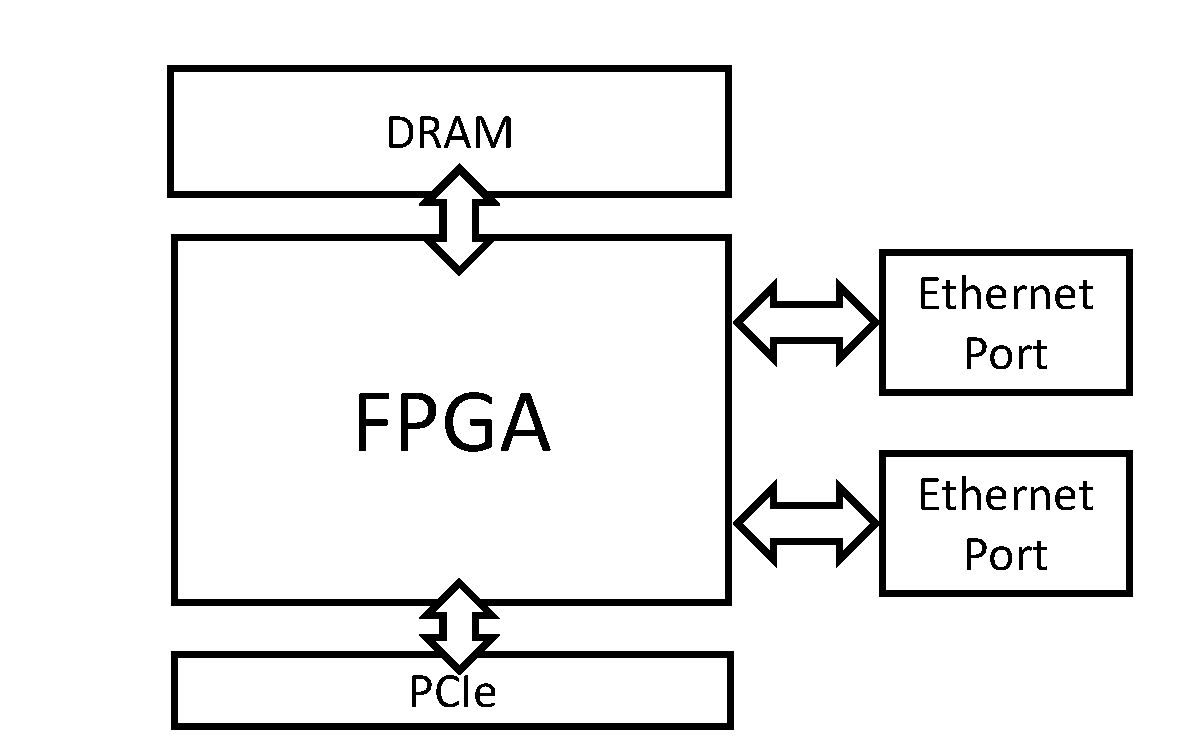
\includegraphics[width=0.6\textwidth]{fpga-board.pdf}
	
	\caption{FPGA板的逻辑图。}
	\label{clicknp:fig:fpga}
	
\end{figure}


与CPU或GPU相比,FPGA通常具有更低的时钟频率和更小的存储器带宽。
例如,FPGA的典型时钟频率约为200MHz,比CPU慢一个数量级(2至3~GHz)。
同样,FPGA的单块存储器或外部DRAM的带宽通常为2至10~GBps,而内存带宽约为Intel XEON CPU的40~GBps,GPU为100~GBps。
但是,CPU或GPU只有有限的内核,这限制了并行性。 FPGA内置了大量的并行性。
现代FPGA可能拥有数百万个LE,数百个K位寄存器,数十个M位BRAM和数千个DSP模块。从理论上讲,它们中的每一个都可以并行工作。
因此,FPGA芯片内部可能会同时运行数千个并行的``\textit {核}''。
虽然单个BRAM的带宽可能有限,但如果我们并行访问数千个BRAM,则总内存带宽可以是多TBps!
因此,为了实现高性能,程序员必须充分利用这种大规模的并行性。

传统上,FPGA使用诸如Verilog和VHDL之类的HDL进行编程。
这些语言水平太低,难以学习,编程也很复杂。
因此,大型软件程序员社区已经远离FPGA多年了~\cite {bacon2013fpga}。
为了简化这一点,许多高级综合(HLS)工具/系统已经在工业界和学术界开发,试图将高级语言(主要是C)的程序转换为HDL。
但是,正如我们将在第 \ref{chapter:clicknp} 章中看到的,它们都不适合网络功能处理,这是本工作的重点。


\subsection{架构对比}
\label{smartnic-comparison}

性能逐渐降低,可编程性逐渐提高。

如何选择,考虑几个方面:

\section{可编程网卡在数据中心的应用}
\label{background:sec:application}


\subsection{微软 Azure 云}

\begin{figure}[htbp]
	\centering
	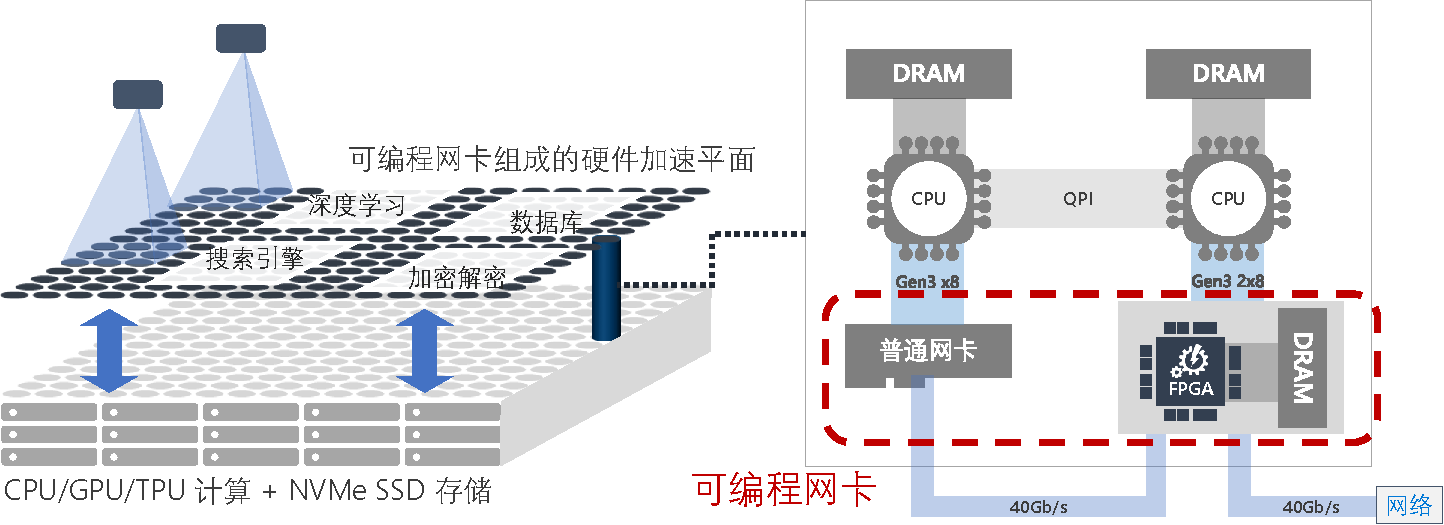
\includegraphics[width=0.8\textwidth]{figures/azure_fpga.pdf}
	\caption{微软基于 FPGA 的可编程网卡。}
	\label{background:fig:azure_fpga}
\end{figure}


New content:

1. CPU - accelerator communication
1) coherent memory
2) I/O DMA
3) Network

2. connectivity among accelerators
1) single server
2) rack
3) data center

3. device
1) FPGA
2) GPU
3) ASIC

New workloads:

compute offload

1) bing: hardware microservice, consolidation

2) compression and encryption: Office 365, Cosmos/Azure data lake, Onedrive

3) AI inference: neural networks, traditional models, AAAI'18

4) 3rd party: general computing acceleration device

infrastructure offload: (pioneer the wave of SmartNICs)

1) networking: network virtualization (compute node); NFV (network node)

2) persistent storage: SOSP'11; compression and encryption (backend): improve throughput; improve compression ratio, save storage space.
hypervisor and sharing (frontend)



微软对于把 FPGA 部署在哪里这个问题,大致经历了三个阶段:
\begin{enumerate}
	\item 专用的 FPGA 集群,里面插满了 FPGA;
	\item 每台机器一块 FPGA,采用专用网络连接;
	\item 每台机器一块 FPGA,位于网卡和交换机之间,共享服务器网络。
\end{enumerate}

第一个阶段是专用集群,里面插满了 FPGA 加速卡,就像是一个 FPGA 组成的超级计算机。像超级计算机一样的部署方式有几个问题:

\begin{enumerate}
	\item 不同机器的 FPGA 之间无法通信,FPGA 所能处理问题的规模受限于单台服务器上 FPGA 的数量;
	\item 数据中心里的其他机器要把任务集中发到这个加速机柜,构成了 in-cast 的网络流量特征,网络延迟很难做到稳定;
	\item FPGA 专用机柜构成了单点故障;
	\item 装 FPGA 的服务器是定制的,散热设计和运维都增加了复杂性。
\end{enumerate}

一种不那么激进的方式是,在每个机柜一面部署一台装满 FPGA 的服务器。这避免了上述问题 (2)(3),但(1)(4) 仍然没有解决。

第二个阶段,为了保证数据中心中服务器的同构性(这也是不用 ASIC 的一个重要原因),在每台服务器上插一块FPGA,FPGA 之间通过专用网络连接。这也是微软在 ISCA’14 上所发表论文采用的部署方式。

FPGA 采用Stratix V D5,有172K个ALM,2014个M20K片上内存,1590个 DSP。板上有一个8GB DDR3-1333 内存,一个PCIe Gen3 x8接口,两个10 Gbps网络接口。一个机柜之间的FPGA采用专用网络连接,一组10G网口8个一组连成环,另一组10G网口6个一组连成环,不使用交换机。

这样一个 1632 台服务器、1632 块 FPGA 的集群,把必应的搜索结果排序整体性能提高到了 2倍(换言之,节省了一半的服务器)。本地和远程的 FPGA 均可以降低搜索延迟,远程 FPGA的通信延迟相比搜索延迟可忽略。[4]

FPGA 在必应的部署取得了成功,Catapult 项目继续在公司内扩张。微软内部拥有最多服务器的,就是云计算 Azure 部门了。Azure 部门急需解决的问题是网络和存储虚拟化带来的开销。Azure把虚拟机卖给客户,需要给虚拟机的网络提供防火墙、负载均衡、隧道、NAT等网络功能。由于云存储的物理存储跟计算节点是分离的,需要把数据从存储节点通过网络搬运过来,还要进行压缩和加密。

为了加速网络功能和存储虚拟化,微软把 FPGA 部署在网卡和交换机之间。一块 FPGA(加上板上内存和网络接口等)的功耗大约是30 W,仅增加了整个服务器功耗的十分之一。只要规模足够大,对FPGA价格过高的担心将是不必要的。每个 FPGA 有一个 4GB DDR3-1333 DRAM,通过两个 PCIe Gen3 x8 接口连接到一个 CPU socket(物理上是 PCIe Gen3 x16 接口,因为 FPGA 没有 x16 的硬核,逻辑上当成两个 x8 的用)。物理网卡(NIC)就是普通的 40 Gbps 网卡,仅用于宿主机与网络之间的通信。


\textbf{图:微软SmartNIC可编程网卡的架构,其中FPGA位于网络和经典网卡之间}

FPGA(SmartNIC)对每个虚拟机虚拟出一块网卡,虚拟机通过 SR-IOV直接访问这块虚拟网卡。原本在虚拟交换机里面的数据平面功能被移到了 FPGA 里面,虚拟机收发网络数据包均不需要 CPU参与,也不需要经过物理网卡(NIC)。这样不仅节约了可用于出售的 CPU 资源,还提高了虚拟机的网络性能(25 Gbps),把同数据中心虚拟机之间的网络延迟降低了 10 倍。

这就是微软部署 FPGA 的第三代架构,也是目前「每台服务器一块 FPGA」大规模部署所采用的架构。FPGA 复用主机网络的初心是加速网络和存储,更深远的影响则是把 FPGA 之间的网络连接扩展到了整个数据中心的规模,做成真正 cloud-scale 的「超级计算机」。第二代架构里面,FPGA 之间的网络连接局限于同一个机架以内,FPGA之间专网互连的方式很难扩大规模,通过 CPU 来转发则开销太高。

第三代架构中,FPGA 之间通过 LTL (Lightweight Transport Layer) 通信。同一机架内延迟在 3微秒以内;8 微秒以内可达 1000 块 FPGA;20 微秒可达同一数据中心的所有 FPGA。第二代架构尽管 8台机器以内的延迟更低,但只能通过网络访问 48 块 FPGA。为了支持大范围的 FPGA 间通信,第三代架构中的 LTL 还支持PFC 流控协议和 DCQCN 拥塞控制协议。

通过高带宽、低延迟的网络互连的 FPGA构成了介于网络交换层和传统服务器软件之间的数据中心加速平面。除了每台提供云服务的服务器都需要的网络和存储虚拟化加速,FPGA上的剩余资源还可以用来加速必应搜索、深度神经网络(DNN)等计算任务。

对很多类型的应用,随着分布式 FPGA 加速器的规模扩大,其性能提升是超线性的。例如 CNN inference,当只用一块 FPGA 的时候,由于片上内存不足以放下整个模型,需要不断访问 DRAM 中的模型权重,性能瓶颈在DRAM;如果 FPGA 的数量足够多,每块 FPGA 负责模型中的一层或者一层中的若干个特征,使得模型权重完全载入片上内存,就消除了DRAM 的性能瓶颈,完全发挥出 FPGA 计算单元的性能。当然,拆得过细也会导致通信开销的增加。把任务拆分到分布式 FPGA集群的关键在于平衡计算和通信。

在 MICRO’16 会议上,微软提出了 Hardware as a Service(HaaS) 的概念,即把硬件作为一种可调度的云服务,使得 FPGA服务的集中调度、管理和大规模部署成为可能。


2016 年 9 月,《连线》(Wired)杂志发表了一篇《微软把未来押注在 FPGA 上》的报道 [3],讲述了 Catapult 项目的前世今生。紧接着,Catapult 项目的负责人 Doug Burger 在 Ignite 2016 大会上与微软 CEO Satya Nadella 一起做了 FPGA 加速机器翻译的演示。演示的总计算能力是 103 万 T ops,也就是 1.03 Exa-op,相当于 10 万块顶级 GPU 计算卡。



\subsection{亚马逊 AWS 云}

在 2017 年 12 月的 Re:Invent 大会上,亚马逊 AWS 云发布了名为 ``Nitro'' 的计算加速架构 \cite{nitro-blog}。
根据 2017 年 Re:Invent 大会和 2018 年 AWS 峰会上亚马逊发布的信息 \cite{nitro-talk,nitro-web},AWS 使用了定制 ASIC 来实现多种加速和安全功能。
最初,AWS 在 FPGA 和 ASIC 架构之间权衡,并决定采用 ASIC 方案。
为此,2015 年 1 月,亚马逊用 30 多亿美元收购了 ASIC 设计公司 Annapurna 实验室 \cite{annapurna},该公司以设计基于 ARM 核的片上系统(SoC)见长。

Nitro 项目的发展是分阶段的。与微软 Azure 类似,虚拟机的 I/O 瓶颈最早体现在虚拟网络上。早在 2013 年 11 月,AWS 的 C3 实例就引入了一块独立的网卡以实现高性能网络(enhanced networking),采用 SR-IOV 方式让虚拟机直接访问网卡,绕过虚拟机监控器中的虚拟交换机软件。此技术帮助 Netflix 实现了每秒 200 万个数据包的虚拟机网络吞吐量 \cite{netflix-aws}。

2015 年 1 月,AWS 的 C4 实例开始使用硬件加速弹性块存储(Elastic Block Storage,EBS)。弹性块存储的数据储存在存储节点上,而客户虚拟机运行在计算节点上,因此这是一种远程存储。对客户虚拟机而言,是一块虚拟存储设备,它是由虚拟机监控器 Xen Dom0 中的存储管理软件实现虚拟化的。C4 实例使用高性能网卡而非传统网卡来连接远程的弹性块存储,从而提高了性能。

2017 年 2 月,AWS 的 I3 实例引入了 NVMe 本地存储和专用的存储虚拟化芯片。以往,客户虚拟机访问本地存储,也需要经过虚拟机监控器中的存储管理软件,这是由于一台物理服务器中可能有多台虚拟机,每台虚拟机只能访问属于自己的那一部分存储空间,因此需要隔离。对延迟和吞吐量都很高的 NVMe 存储而言,存储虚拟化软件带来的开销太高了。为此,I3 实例引入的 Nitro 芯片在硬件上实现了存储隔离,因此可以通过 SR-IOV 把 NVMe 存储直通客户虚拟机,实现了每秒 300 万次 I/O 操作的存储性能 \cite{aws-local-storage}。

2017 年 11 月,AWS 的 C5 实例大幅改变了计算节点虚拟化的架构。首先,C4 实例中的远程存储仍然需要软件实现虚拟化,这一部分也可以像 I3 本地存储一样用硬件实现,不过块存储比本地存储的接口更复杂,因此硬件实现的难度更大。其次,在网络、远程和本地存储都已经使用硬件虚拟化后,事实上虚拟机监控器中的管理软件就只剩下数据平面的中断(APIC)功能和控制平面的管理功能了。控制平面的管理功能较为复杂,用纯数字逻辑显然是不现实的。为了把虚拟网络(VPC)、弹性块存储和虚拟化控制平面全部卸载(offload)到加速卡上,Nitro ASIC 采用了基于 ARM 核的片上系统架构,从而保持了数据平面的可编程性和灵活性,还能把控制平面一并卸载到加速卡上。

采用 Nitro 加速卡后,AWS 重新设计了一个轻量级的虚拟机监控器 Nitro 来取代 Xen,而原来运行在 Xen Dom0 上的控制平面转移到了 Nitro ASIC 里,客户虚拟机可以得到接近裸金属(bare-metal)主机的性能。此后,AWS 发布了裸金属实例,客户代码直接在物理机上运行,而所有的存储和网络资源都由 Nitro 卡提供。

Nitro 系列芯片主要包括三种芯片 \cite{nitro-blog,nitro-talk,nitro-web}:
\begin{enumerate}
	\item 云网络(VPC)和弹性块存储(EBS)加速芯片,一边连接数据中心网络,一边以 PCIe 卡的形式连接 CPU;
	\item 本地 NVMe 存储虚拟化芯片,作为 CPU 和 NVMe 存储设备之间的代理;
	\item 安全芯片,用于验证服务器中各种设备固件的版本,以及在裸金属服务器切换租户时重刷固件清除痕迹。
\end{enumerate}

Nitro 芯片的作用可以分为降低成本、提高性能和提高安全性三方面。下面详细讨论。

\textbf{节约 CPU 核。}
网络和存储虚拟化需要占用大量的 CPU 资源来处理每个网络包和存储 I/O 请求。
根据 ClickNP \cite{li2016clicknp} 估计,每个客户虚拟机的 CPU 核,需要预留另外 0.2 个 CPU 核来实现虚拟化。
如果这些功能可以被卸载到专用硬件,所节省的 CPU 核就可以用来安装客户虚拟机。
不管是考虑公有云虚拟机上每个 CPU 核的售价,还是考虑 Xeon CPU 每个核的硬件成本,用专用硬件都能获得明显的成本节约 \cite{smartnic}。

\textbf{提高最大核数。}
节约 CPU 核不仅能够降低成本,还能够提高大型虚拟机实例的最大核数。因为各大公有云厂商都从 Intel 等相同的厂商购买 CPU,因此同一时期能买到的最大 CPU 核数是相对固定的。虚拟化被卸载到硬件后,所有 CPU 核都用于运行客户虚拟机,因此 AWS 的 M5 实例最多可达 96 个 CPU 核。如果不使用硬件卸载,将只有 80 个 CPU 核可用于客户虚拟机,从而降低对追求极致性能客户的吸引力。

\textbf{提高单核频率。}
由于功耗墙的限制,CPU 的核心数目与平均核心频率不可兼得。同一代 CPU 架构下,较高核心频率的 CPU 核数一般较少。对于核数相等的虚拟机实例,如果使用传统的软件虚拟化,物理机就需要 1.2 倍的 CPU 核数,从而平均核心频率就可能降低。例如,在 C5 实例推出前的 72 核 EC2 实例,CPU 基频为 2.7 GHz,但采用同一代 Skylake 架构的 C5 实例虚拟机,CPU 基频就可以达到 3.0 GHz。

\textbf{提高本地存储性能。}
首先,在裸金属服务器上,本地 NVMe 存储可以达到每盘高达 400 K IOPS(I/O 操作每秒)的吞吐量。AWS I3 实例有 8 块 NVMe SSD,达到 3 M IOPS 的吞吐量。而对于常见的存储虚拟化协议栈,每个 CPU 核只能处理 100 K IOPS 左右的吞吐量,这意味着要占用 30 个 CPU 核才能让虚拟机充分利用 NVMe 存储的吞吐量,这个开销太高了。即使只有一块 NVMe 存储,4 个 CPU 核之间的负载均衡仍然是个难题 \cite{li2017kv}。如第 \ref{smartnic-architecture} 节所讨论的,由于硬件分配和处理任务是流水线式而非多个处理单元简单并行,硬件能够比多核软件更好地保证服务质量(QoS)。

其次,在延迟方面,裸金属服务器的 NVMe 存储平均延迟约为 80 微秒。虚拟化软件不仅会增加 20 微秒的平均延迟,而且由于操作系统调度、中断、缓存不命中等因素的影响,在高负载下的尾延迟(tail latency)可高达 1 毫秒(1000 微秒)。采用硬件卸载可以降低平均延迟 20\%,并降低高负载下的尾延迟 90\% 以上。

\textbf{提高远程存储性能和安全性。}
与本地存储类似,硬件加速可以提高远程存储性能。还有一点额外的优势:远程存储被公有云的所有租户共享,对可靠性和安全性要求更高。传统上远程存储协议在虚拟机监控器中运行,虽然逻辑上与客户虚拟机隔离,但由于共享 CPU、内存等资源,仍然不能排除零日(0-day)漏洞和边信道攻击的潜在安全隐患。把远程存储协议从主机 CPU 卸载到 Nitro 卡后,就有了更高的隔离性和更小的攻击表面(attack surface)。

\textbf{提高网络性能和安全性。}
在 Nitro 卡上实现网络虚拟化后,虚拟机可以直接通过 SR-IOV 访问网卡,达到数据中心网络 25 Gbps 的理论上限,尤其是对小数据包应用场景的性能提升明显。根据 ClickNP \cite{li2016clicknp} 估计,对 25 Gbps 线速(line-rate)的 64 字节小数据包,每秒高达 37 百万个,如果用软件虚拟交换机处理,将需要 60 个 CPU 核,这显然是不可接受的。因此大多数云服务商对虚拟网络(VPC)对吞吐量不仅有字节数的限制,还有数据包数的限制。大多数公有云的虚拟网络只支持数百万数据包每秒的吞吐量,需要处理大量小请求的远程过程调用(RPC)、键值存储(KVS)服务器就会遇到性能瓶颈。在延迟方面,软件虚拟化的 AWS 端到端延迟可达 100 微秒以上,而使用 Nitro 虚拟化加速后延迟就降低到 50 微秒以内了。硬件虚拟化对虚拟网络的尾延迟、服务质量和安全性的提升,也与远程存储相似。

\textbf{提高裸金属服务器安全性。}
最后,裸金属服务器上的客户代码可以直接访问服务器内的各种硬件设备,甚至可能烧写带外服务器管理(BMC)等组件的固件 \cite{bare-metal-security}。如果固件内被嵌入了恶意代码,并在下一个租户使用该裸金属服务器时被激活,后果不堪设想。事实上很大一部分客户选择裸金属服务器,正是出于对虚拟机隔离性的担忧。为了在租户开始使用裸金属服务器时提供安全和一致的硬件环境,Nitro 安全芯片会对固件进行重烧写。Nitro 还会在系统启动时进行完整性检查,这类似 UEFI 可信启动技术,但验证的范围不仅包括操作系统引导器,还包括硬件固件。

\subsection{阿里云、腾讯云、华为云}

2018 年,我国云计算服务商也积极地在数据中心部署了可编程网卡。阿里云和腾讯云部署可编程网卡的首要目的是支持裸金属(bare-metal)服务器。相比虚拟机,裸金属服务器可以消除虚拟化带来的开销,实现同样硬件条件下最高的性能;方便部署客户自己的虚拟化软件(如 VMWare);与客户在自有数据中心(on-premises)的部署环境完全相同,降低客户上云的迁移开销;方便使用不支持虚拟化或虚拟化后性能有较大损失的硬件,如 GPU 和 RDMA 网卡;不与其他租户共享服务器硬件,隔离性和安全性更强,也能符合一些客户的合规要求。

在公有云中使用裸金属服务器的主要技术挑战是访问数据中心内的虚拟网络(VPC)和远程存储(EBS)等资源。一种简单的方法是在同一个机架(rack)内放置若干虚拟网络和存储服务器,部署相应的软件;并在柜顶交换机(ToR switch)上配置转发规则,使裸金属服务器的所有网络数据包经过虚拟网络和存储服务器。这种方法需要增加额外的服务器资源,提高了成本。另一种方法是把虚拟网络和存储的数据平面卸载到柜顶交换机上。但是,柜顶交换机的编程灵活性一般较差 \cite{tencent-smartnic},不足以支持虚拟存储的应用层协议和虚拟网络的安全规则等。

因此,在服务器上增加一块可编程网卡便成为支持裸金属服务器性能最高的方案。阿里和腾讯采用了 FPGA 数据平面与多核 CPU 控制平面结合的 SoC 方案。2018 年,阿里云发布的 ``神龙'' 裸金属服务器使用自研的 MOC 卡 \cite{alicloud-smartnic,alicloud-xdragon} 实现类似 AWS Nitro 的网络、存储虚拟化。腾讯云在 APNet’18 上发布了基于 FPGA 的可编程网卡方案,主要用于网络虚拟化 \cite{tencent-smartnic}。腾讯仅用 10 个硬件工程师,就在三个月内完成了 FPGA 逻辑设计,用四个月做出了可编程网卡的板卡,并在一年内部署 \cite{tencent-smartnic}。这是 FPGA 编程也可以实现敏捷开发的例证。腾讯正在把可编程网卡的应用范围从裸金属服务器扩展到普通虚拟机,并对两种应用场景使用统一的可编程网卡架构。

华为基于海思半导体的技术积累,发布了两款可编程网卡,同时也用于华为云虚拟网络的加速。SD100 系列可编程网卡 \cite{sd100} 采用了基于多核 ARM64 CPU 的 SoC 架构,数据平面和控制平面都运行在 ARM CPU 上。IN5500 系列可编程网卡 \cite{in200} 采用网络处理器(NP)提供数据平面的可编程性,可达到 100 Gbps 性能。利用可编程网卡,华为云发布了 C3ne 网络增强虚拟机实例,在国内云厂商中率先实现了每秒千万级的数据包转发 \cite{huawei-smartnic}。

%!TEX root=main.tex
\section{架构}
\label{clicknp:sec:architecture}

\subsection{系统架构}
\label{clicknp:subsec:sysarch}

图 \ref{clicknp:fig:clicknp} 显示了 \name 的体系结构。
\name 以 Catapult Shell 架构构建\cite {putnam2014reconfigurable}。
\textit {shell}包含许多可重用的逻辑位,这些逻辑对所有应用程序都是通用的,并将它们抽象为一组明确定义的接口,例如,PCIe,直接内存访问(DMA),DRAM内存管理单元(MMU),和以太网MAC。
\name FPGA程序合成为 Catapult \textit {role}。
但是,由于\name 依赖于商品高层次综合工具链来生成FPGA 硬件描述语言,并且不同的工具可以为shell管理的资源生成自己的(和不同的)接口,需要一个名为\textit {高层次综合-的垫片层特定运行时},用于执行高层次综合特定接口与shell接口之间的转换。


\begin{figure}
	\centering
	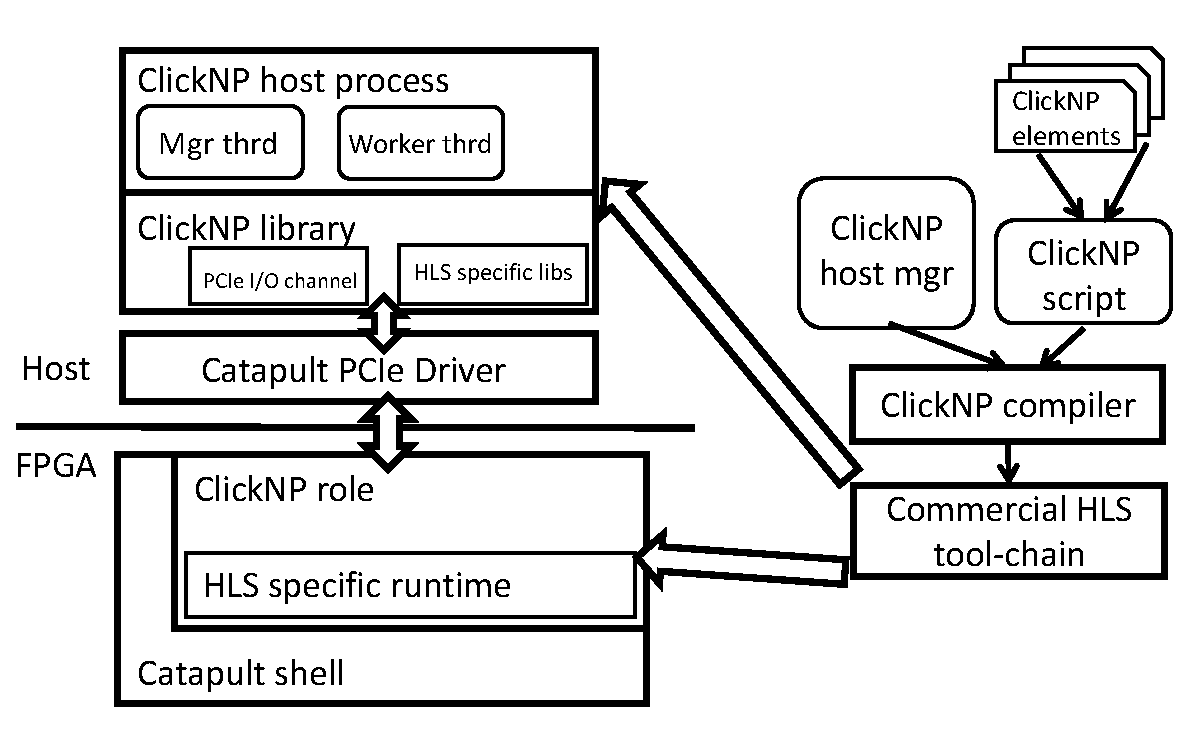
\includegraphics[width=.8\textwidth]{clicknp-arch.pdf}
	\caption{ClickNP 架构。}
	\label{clicknp:fig:clicknp}
\end{figure}


\name{} host 进程通过 \name{} library与 \name{} role 进行通信,这进一步依赖于 Catapult PCIe 驱动程序中的服务与FPGA硬件进行交互。
\name{} library 实现了两个重要的功能:
(1)它暴露了一个PCIe通道API,以实现 \name{} host进程和角色之间的高速和低延迟通信;
(2)它调用几个高层次综合特定库将初始参数传递给角色中的模块,并控制这些模块的启动/停止/复位。
\name{} host进程有一个管理器线程和零个或多个工作线程。
管理器线程将FPGA映像加载到硬件中,启动工作线程,根据配置初始化FPGA和CPU中的\name elements,并通过在运行时向元件发送\textit {signals}来控制它们的行为。
如果将每个工作线程分配给CPU,则每个工作线程可以处理一个或多个模块。

\subsection{\name 编程}

\subsubsection{抽象}

\name 提供模块化架构,基本处理模块称为\textit{元件}(element)。
如图 \ref{clicknp:fig:element_arch} 所示,\name 元件具有以下属性:
\begin{itemize}
\item 本地状态。 每个元件都可以定义一组只能在元件内部访问的局部变量。
\item 输入和输出端口。 元件可以具有任意数量的输入或输出端口。
\item 处理程序功能。 元件有三个处理函数:(1)初始化处理程序,在元件启动时调用一次,(2)处理处理程序,连续调用以检查输入端口和处理可用数据,以及(3)信号处理程序 ,它从主机程序中的管理器线程接收和处理命令(\textit {信号})。
\end{itemize}

\begin{figure}
\centering
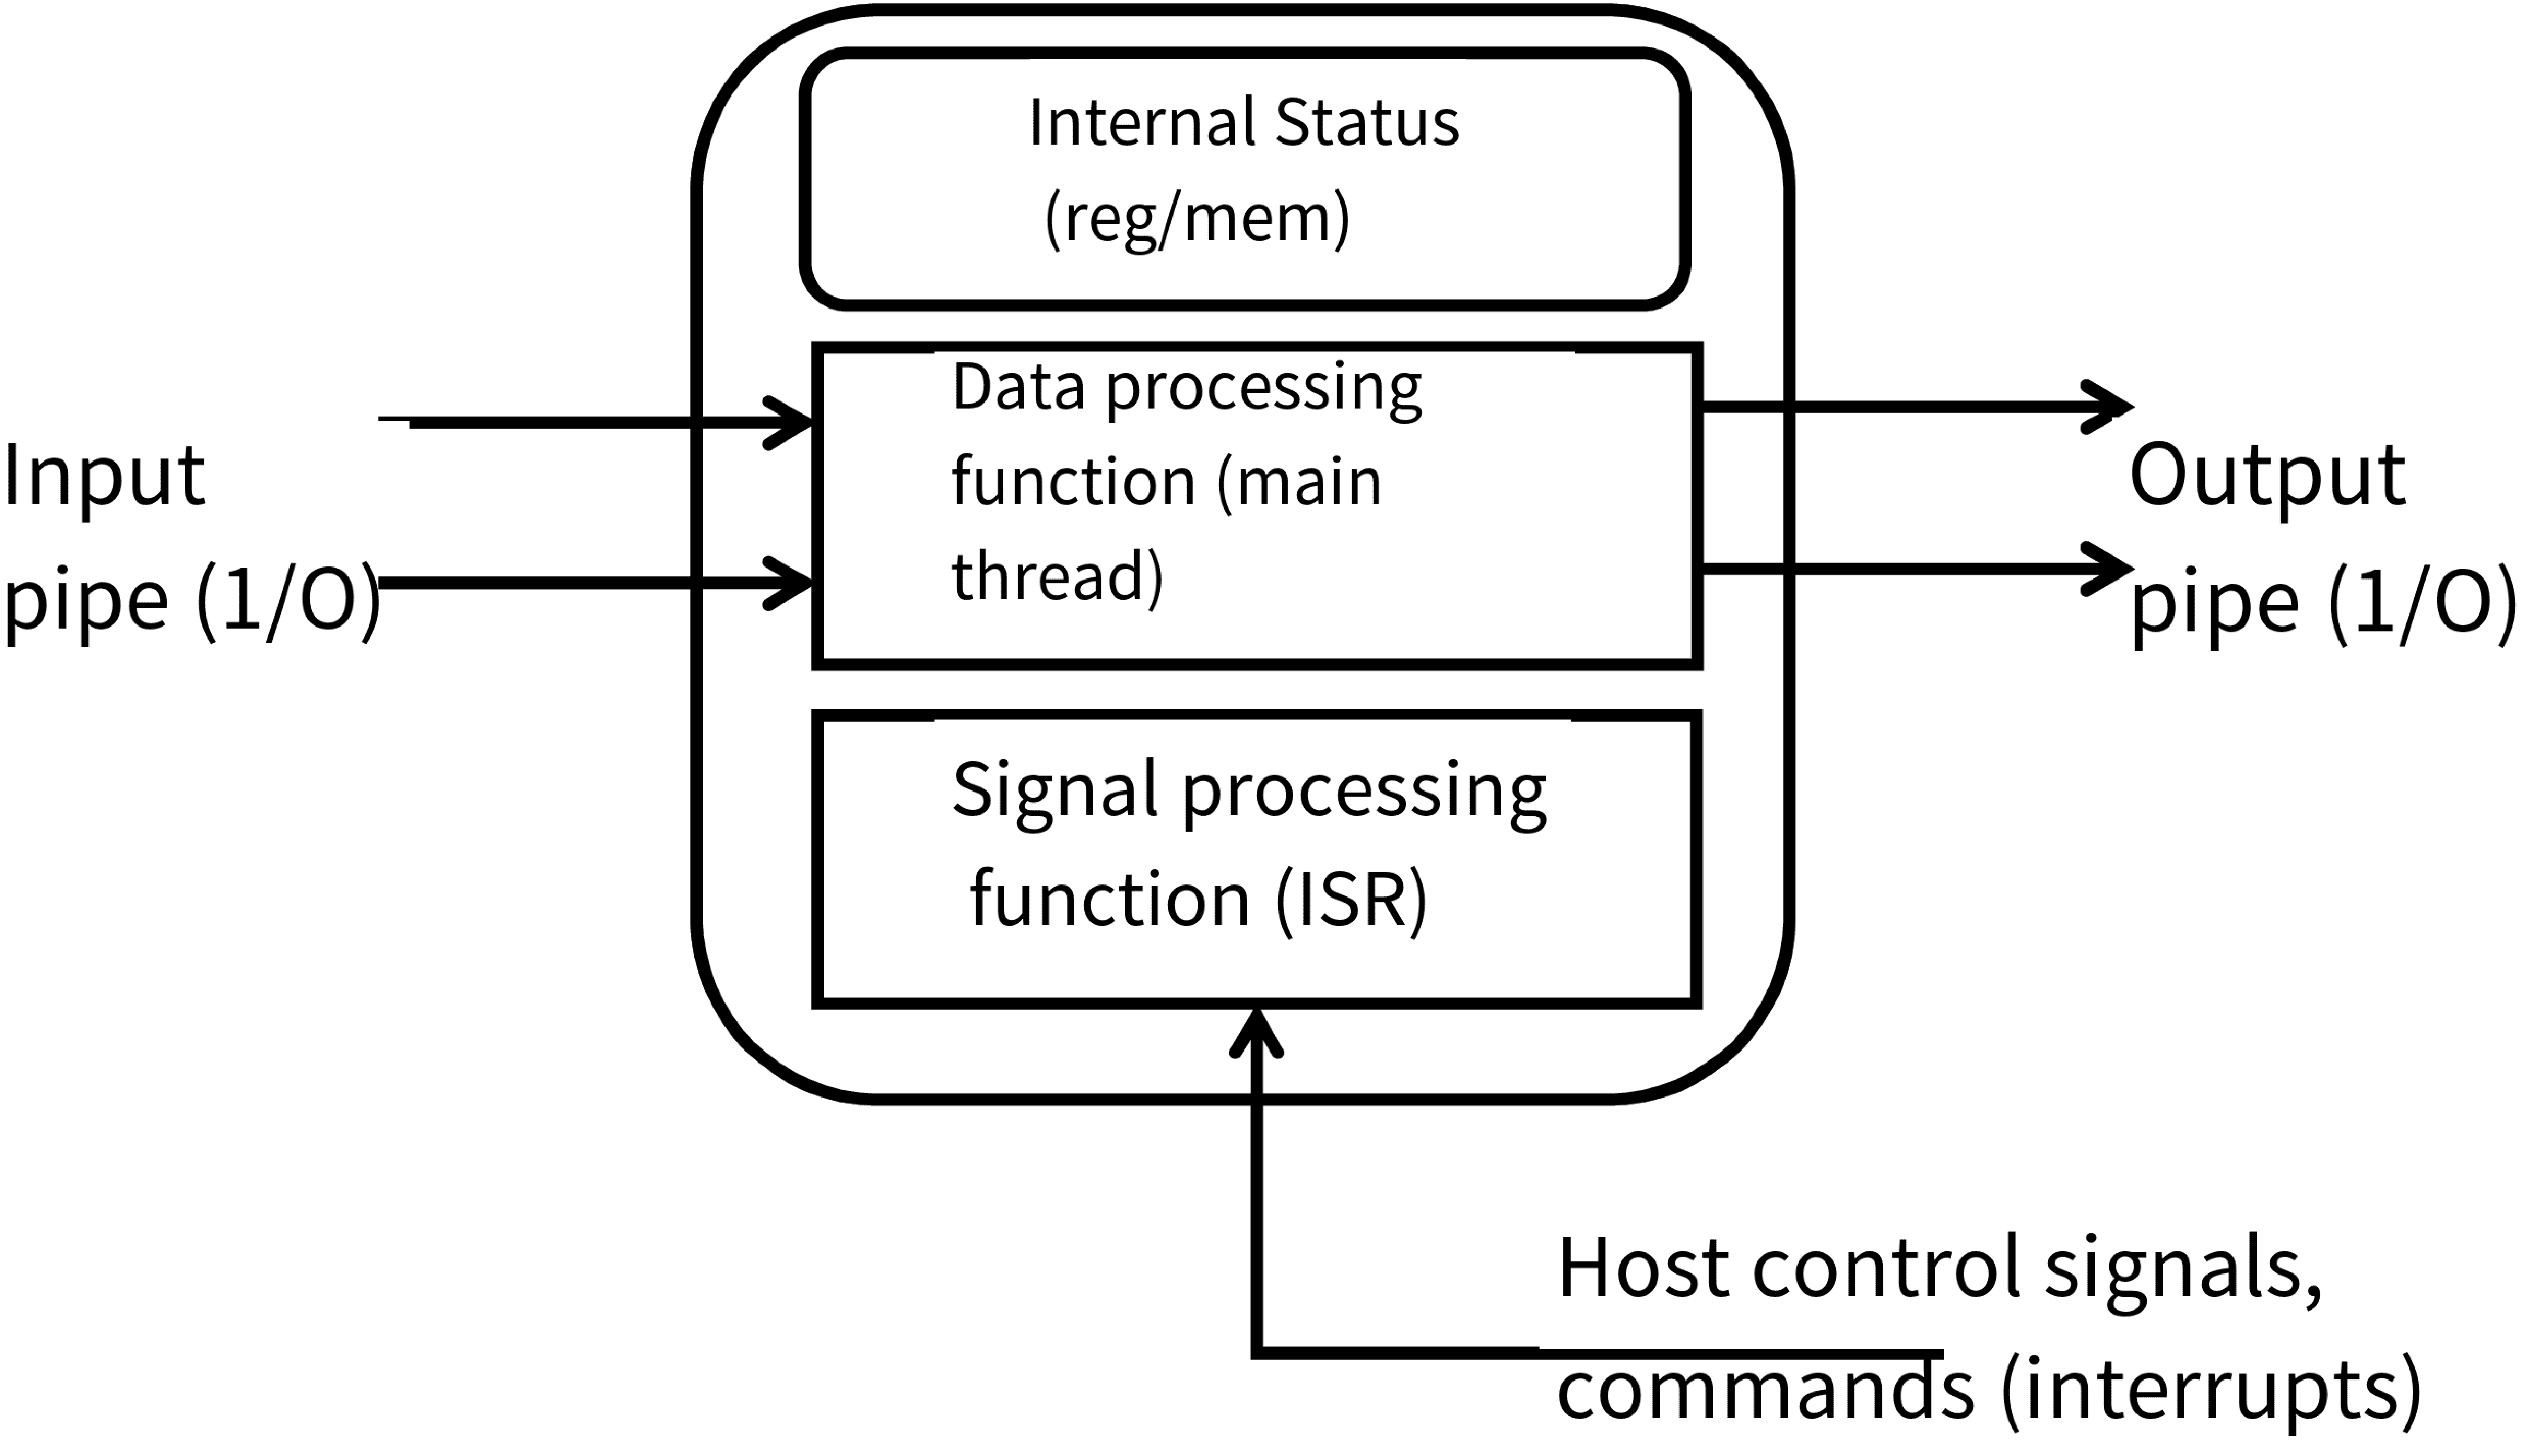
\includegraphics[width=.6\textwidth]{element_arch.pdf}
\caption{ClickNP 元件的构成。}
\label{clicknp:fig:element_arch}
\end{figure}

元件的输出端口可以通过\textit {channel}连接到另一个元件的输入端口,如图\ref {clicknp:fig:element}(a)所示。
在 \name 中,通道基本上是一个FIFO缓冲区,写入一端并从另一端读取。
对通道的读/写操作的数据单元称为 \textit {flit},其具有64字节的固定大小。
flit的格式如图 \ref {clicknp:fig:element}(b)所示。每个flit包含元数据的标头和32字节的有效负载。
当在 \name elements之间流动时,大量数据(例如,完整大小的数据包)被分成多个flits。
第一个flit标有 \textbf {sop}(数据包开始),最后一个flit标有 \textbf {eop}(数据包结束)。
如果数据块的大小不是32,则最后一个flit的 \textbf {pad}字段表示已填充到有效负载的字节数。
通过硬件描述语言综合工具优化了flit中的保留字段。
将大数据分解为flits不仅可以减少延迟,还可以在不同元件处同时处理分组的不同片段,以增加并行性。
最后,为了实现网络功能,可以将多个\name 元件互连以形成定向处理图,称为\name \textit {配置}。

显然,\name 编程抽象很像Click软件路由器 \cite {kohler2000click}。
但是,有三个基本差异使得 \name 更适合FPGA实现:
(1)在Click中,元件之间的边是C ++函数调用,并且需要\textit {queue}元件来存储数据包。
但是,在 \name 中,边实际上表示可以保存实际数据的FIFO缓冲区。此外,\name  channels打破了元件之间的数据依赖关系,并允许它们并行运行。
(2)与Click不同,其中每个输入/输出端口可以是\textit {push或pull},\name 统一了这些操作:一个元件只能\textit {write(push)}到任何输出端口,而 \textit {read(pull)}可以从任何输入端口执行此操作。
(3)Click允许元件直接调用另一个元件的方法(通过基于流的路由器上下文),在 \name 中元件之间的协调是\textit {基于消息},例如,请求者向响应者发送请求消息并通过另一个消息获得响应。
与通过共享内存进行协调相比,基于消息的协调允许更多的并行性并且在FPGA中更有效,其中访问共享内存位置必须被序列化并且将成为瓶颈。
\begin{figure}
\centering
\begin{tabular}{c}
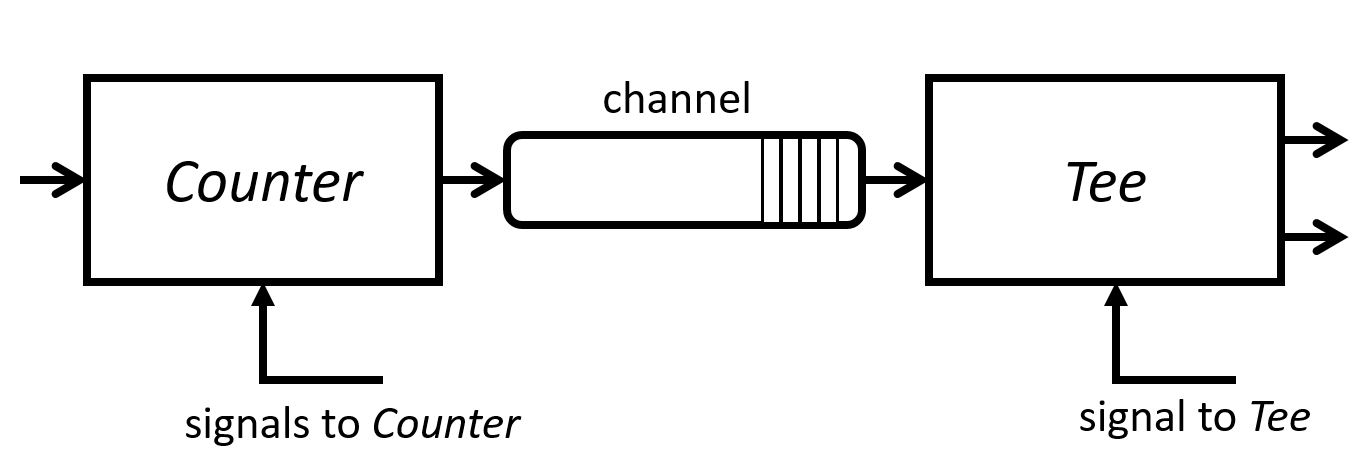
\includegraphics[width=.7\textwidth]{element.jpg}  \\
(a)\\
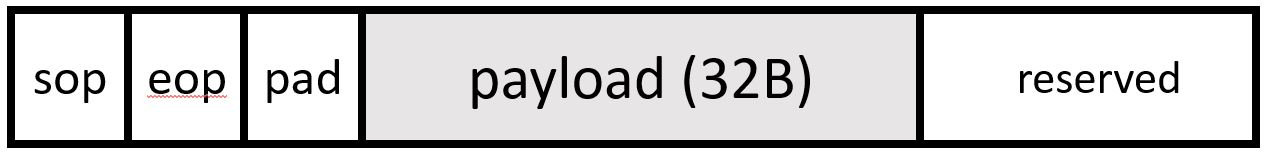
\includegraphics[width=.6\textwidth]{flit.jpg} \\
(b) \\
\end{tabular}

\caption{(a) 两个用管道相连接的 \name 元件。 (b) Flit 的格式。}
\label{clicknp:fig:element}

\end{figure}

\subsubsection{语言}

\name 元件(element)可以声明为面向对象语言(如 C++)中的一个对象。
不幸的是,许多现有的高层次综合工具仅支持C语言。
为了利用商业高层次综合工具,可以编写一个编译器,将面向对象的语言(例如 C++)转换为C,但这种努力并非易事。
本文采用一种替代路径来扩展C语言以支持元件声明。
图 \ref {clicknp:fig:lang}(a)显示了element \textit {Counter}的代码片段,它只计算传递了多少个数据包。元件由 \textbf {.element}关键字定义,后跟元件名称和输入/输出端口数。
关键字 \textbf {.state} 定义元件的状态变量,\textbf {.init},\textbf {.handler} 和 \textbf {.signal}指定初始化,处理和信号处理函数元件。
实现了一组内置函数来对输入和输出端口进行操作,如表 \ref {clicknp:tab:built-in} 中所述。

与Click类似,\name 也使用简单脚本来指定网络功能的配置。配置有两部分:\textit {declarations} 和 \textit {connections},遵循Click语言的类似语法 \cite {kohler2000click}。
值得注意的是,在 \name 中,可以使用关键字 \textbf {host}来注释元件,这将导致元件被编译为CPU二进制文件并在CPU上执行。

\iffalse
\textbf{Verilog 元件。}
\fi

\begin{table}

\centering
\caption{\name\ 管道上的内置操作。}
\label{clicknp:tab:built-in}
\scalebox{0.9}{
\begin{tabular}{p{.4\textwidth}|p{.5\textwidth}}
\toprule
uint get\_input\_port() & 获取具有可用数据的所有输入端口的位图。 \\
\midrule
bool test\_input\_port(uint id) & 测试id指示的输入端口。 \\
\midrule
flit read\_input\_port(uint id) & 读取id指示的输入端口。 \\
\midrule
flit peek\_input\_port(uint id) & 获取id指示的输入端口数据,但不取走。 \\
\midrule
void set\_output\_port(uint id, flit x) & 将flit设置为输出端口。 处理程序返回时,flit将写入管道。\\
\midrule
ClSignal read\_signal() & 从信号端口读取信号。\\
\midrule
void set\_signal(ClSignal p) & 在信号端口上设置输出信号。\\
\midrule
return (uint bitmap) & \textbf{.handler} 的返回值指定下一次迭代时要读取的输入端口的位图。 \\
\bottomrule
\end{tabular}
}
\end{table}

\begin{figure}[htbp]
\small \lstset{style=numbers}

\lstset{ emph={%
 element, init, state, handler, signal,include
}, emphstyle={\bfseries .},
morekeywords={get_input_port,read_input_port,from_tor, to_tor, set_output_port, host, set_signal} 
}
\centering
\begin{tabular}{c}
\small
\begin{lstlisting}
element Count <1, 1> {
  state{
    ulong count;
  }
  init{
    count = 0;
  }
  handler{
    if (get_input_port() != PORT_1) {
      return (PORT_1); 
    }
    flit x;
    x = read_input_port(PORT_1);
    if (x.fd.sop) count = count + 1;
    set_output_port(PORT_1, x);
   
    return (PORT_1);
  }
  signal{
    ClSignal p;
    p.Sig.LParam[0] = count;
    set_signal(p);
  }
}
\end{lstlisting} \vspace{3pt} \\
{\normalsize \centering (a)} \vspace{3pt} \\
\begin{lstlisting}
Count :: cnt @ 
Tee :: tee 
host PktLogger :: logger

from_tor -> cnt -> tee [1] -> to_tor
tee [2] -> logger
\end{lstlisting} \vspace{3pt} \\
{\normalsize \centering (b)} 
\end{tabular}
\caption{用 \name 语言写入元件并指定配置的示例。 使用 \textbf {host}关键字注释的元件在CPU上编译和执行。 用“@”注释的元件需要从管理器线程接收控制信号。
	\textbf {``From\_tor''} 和 \textbf {``to\_tor''}是两个内置元件,代表FPGA上以太网端口的输入和输出。 处理函数的返回值指定了将在下一轮中检查的输入端口的位掩码。}
\label{clicknp:fig:lang}

\end{figure}

\subsubsection{\name\ 工具链}
\label{clicknp:subsec:toolchain}
\name 工具链包含一个 \name 编译器作为前端,一个 C / C++ 编译器(例如,Visual Studio或GCC)和一个高层次综合工具(例如,Altera OpenCL SDK或Xilinx Vivado 高层次综合)作为后端。
如图\ref{clicknp:fig:clicknp}所示,要编写 \name 程序,开发人员需要将代码分为三部分:
(1)一组元件,每个元件实现概念上简单的操作,
(2)指定这些元件之间连接的配置文件,以及(3)主机管理器,它初始化每个元件并在运行时控制它们的行为,例如,根据管理员的输入。
这三部分源代码被送入 \name 编译器并转换为主程序和FPGA程序的中间源文件。
主程序可以由普通的C / C++编译器直接编译,而FPGA程序则使用商业高层次综合工具合成。
现有的商用高层次综合工具可以通过时序分析确定每个元件的最大时钟频率。
然后,\name 处理图的时钟受到图中最慢元件的约束。
另外,高层次综合工具还可以生成优化报告,该报告显示元件中的操作之间的依赖性。如果解析了所有依赖关系并且元件通过在每个时钟周期中处理一个flit来实现最佳吞吐量,则元件是\textit {完全流水线化}的。
\egg{
Our ClickNP architecture is built on state-of-the-art data center reconfigurable hardware (Catapult FPGA \cite{putnam2014reconfigurable}) and FPGA programming framework (Altera OpenCL \cite{singh2011implementing}).

\subsection{Catapult FPGA}

Catapult \cite {putnam2014reconfigurable}是一个可重新配置的硬件,用于在搜索引擎排名中卸载特征提取,特征计算和评分。本章修改硬件以包含两个板载40 GE MAC,因此FPGA可以通过两个40 GE端口接收和发送网络数据包,而无需CPU干预。

\begin{figure}[!t]
	\center
	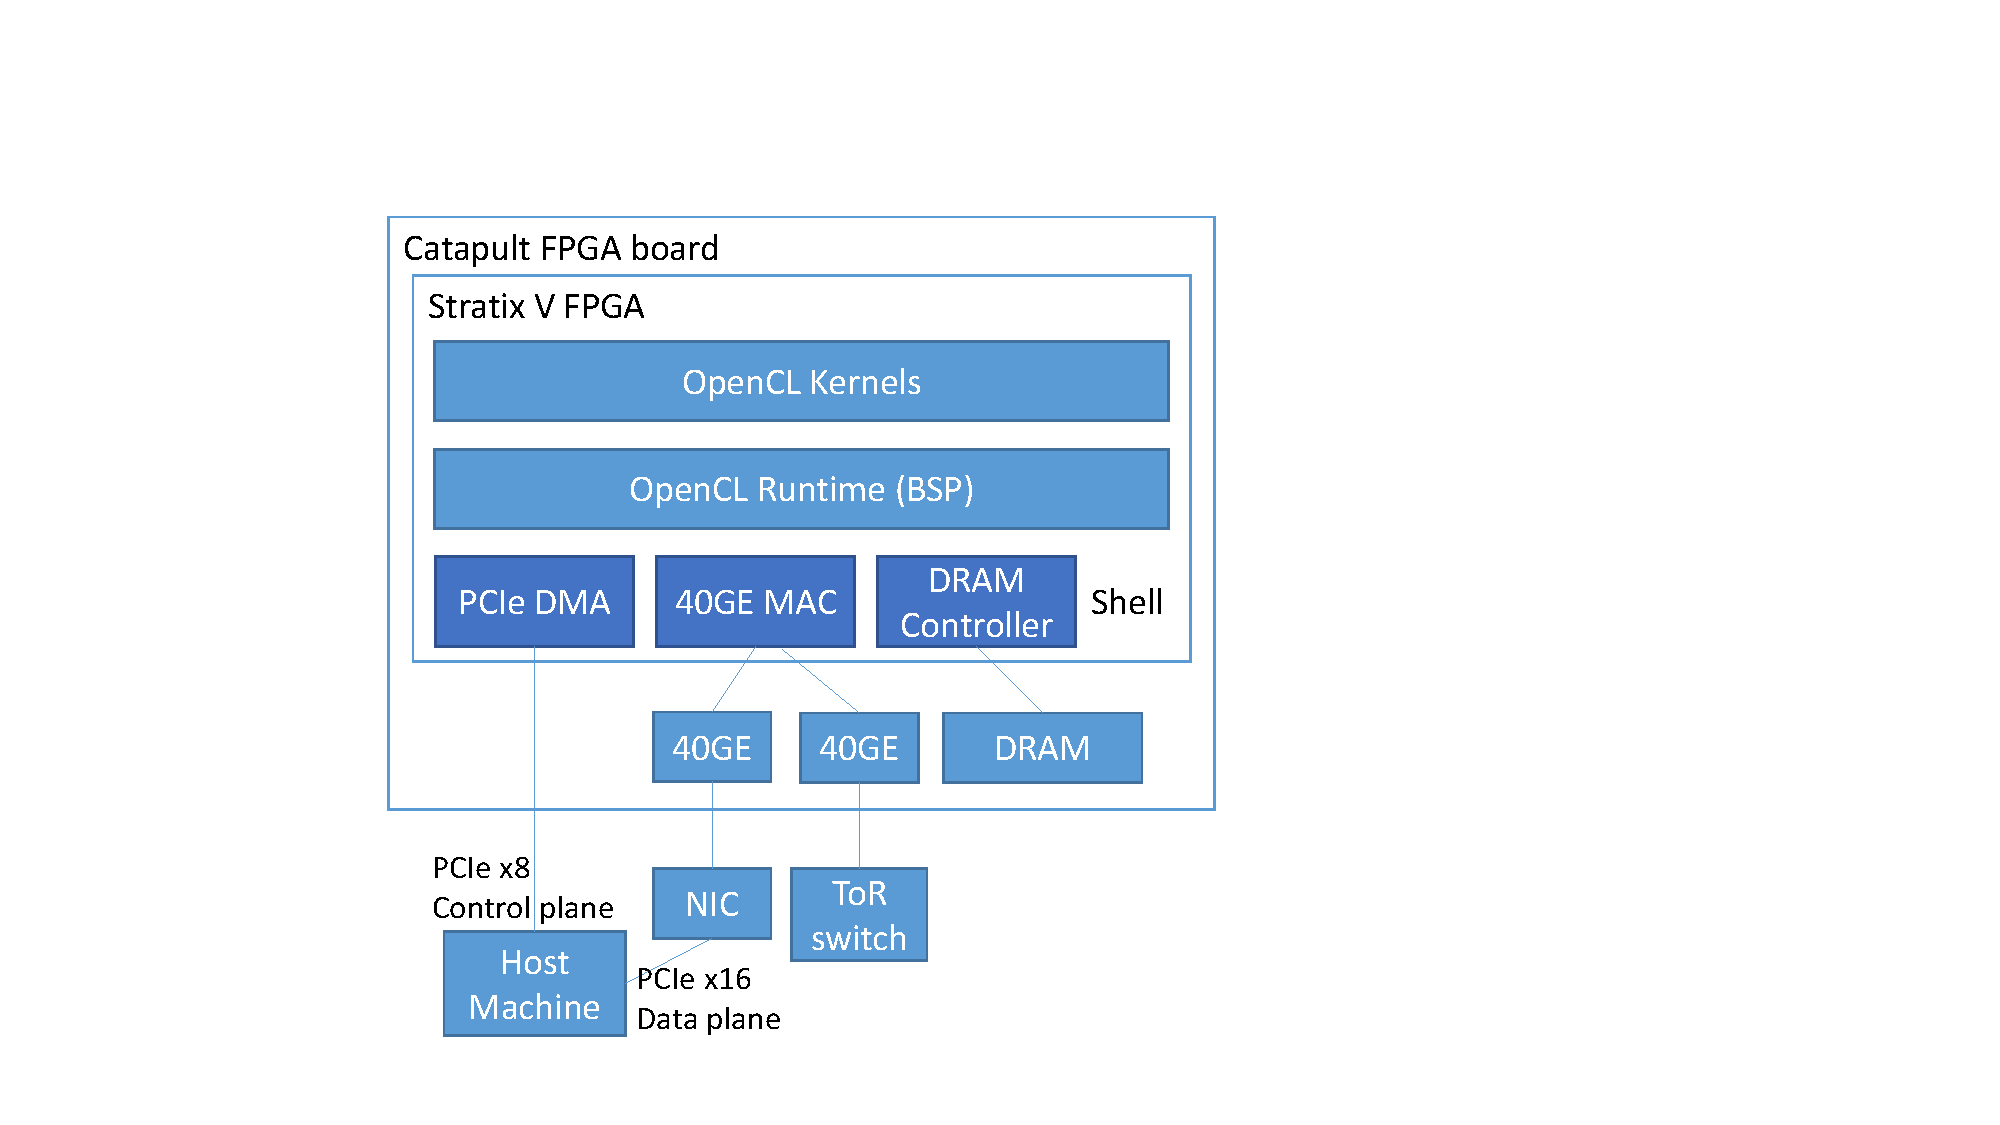
\includegraphics[width=1.0\columnwidth]{image/CatapultFPGAArch}
	\vspace{-0.25in}
	\caption{Catapult FPGA Architecture}
	\vspace{-0.15in}
	\label{clicknp:fig:CatapultFPGAArch}
	%    
\end{figure}

In network virtualization scenario, we install one FPGA in each server and connect two 40 GE ports to 网卡 and Top-of-Rack (ToR) switch respectively. The traffic between 网卡 and ToR flow through the FPGA to perform comprehensive network functions \textit{bump-in-the-wire}, including tunnel encapsulation and decapsulation, firewall, metering and traffic scheduling. Virtual machines expose to the 网卡 and FPGA via Single-Root I/O Virtualization (SR-IOV), and data-plane functions of the virtual switch are offloaded to the FPGA.

Current generation of Catapult FPGA has 172,600 ALMs (Adaptive Logic Modules) each containing several 8-input configurable lookup table, two full adders and four one-bit registers \cite{alterafpgaarch}, 2,014 blocks of 20 Kbit SRAM and a 4 GB DRAM. Each register can be read and written every cycle without latency. Each SRAM block can perform one read or write operation with exactly one cycle latency. The performance of DRAM depends on access pattern. When accessed randomly, each operation takes 170 ns (about 34 cycles); when accessed sequentially, the throughput can reach 4 Gbps. Registers, SRAMs and DRAM form a memory hierarchy where faster memory spaces have lower capacity.

\subsection{OpenCL Compiler}

The Altera SDK for OpenCL \cite{singh2011implementing} is a programming framework that abstract away the traditional hardware FPGA development flow. In the OpenCL \cite{khronos2008opencl} model, data-plane functions are wrapped in \textit{kernels} and compiled into hardware accelerators, and control plane on the host machine communicates with kernels via a standard set of APIs. Altera OpenCL introduces \textit{channels} to allow communication among kernels without host intervention.

Central to Altera OpenCL is a compiler \cite{czajkowski2012opencl} that extracts parallelism in OpenCL kernels and generates Verilog code. A parser based on LLVM first parses OpenCL kernel and produces intermediate representation (IR) consisting of instructions and dependencies between them. Then the IR is optimized via live-variable analysis and generate CDFG (Control Data Flow Graph). Based on CDFG, scheduler determines the required clock cycles of each operation, then sequence the operations into a pipeline, where independent operations are parallelized and dependent operations are pipelined. Finally the compiler links to IP library and generates Verilog 硬件描述语言, as well as a profiling report containing estimated resource utilization and an optimization report containing data dependencies that lead to pipeline stall.

OpenCL is designed primarily for batch processing instead of stream processing, which is a gap that ClickNP needs to bridge. In network stream processing, kernels run in an infinite loop, so the kernels will never finish.

First, when a kernel is running, global memory assigned to it cannot be accessed by the host machine. So commands can not be passed to kernels via global memory on-the-fly. One straightforward approach could be launching another ``proxy'' kernel to pass in commands via channel each time the host sends a command. However, this approach has about 5 millisecond latency due to complicated internals in launching and finishing a kernel. Fortunately, OpenCL only occupies PCIe slots 0--31, so we designed a raw I/O channel via PCIe slots 32--39 to allow on-the-fly interaction of kernels and the host. Figure \ref{clicknp:fig:PCIeChannelPerf} shows that PCIe I/O channels reach near-theoretical throughput with 5 slots and 16K batch size, and the latency for small batch size is microsecond-scale.

\begin{figure}[h!]
	\centering
	\subfigure[Latency (x: batch size, y: microsec; lines: polling, interrupt, opencl)]{
		
\includegraphics[width=0.45\columnwidth]{image/logo}
		\label{clicknp:fig:PCIeChannelLatency}
	}
	\subfigure[Throughput (x : number of slots; y: Gbps; lines: batch size, theory)]{
		
\includegraphics[width=0.45\columnwidth]{image/logo}
		\label{clicknp:fig:PCIeChannelThroughput}
	}
	\vspace{-0.15in}
	\caption{PCIe Channel Performance}
	\vspace{-0.15in}
	\label{clicknp:fig:PCIeChannelPerf}
	%    
\end{figure}

Second, since the kernels never finish, when the host program crashes or need to be updated, although the data plane is still running, we might lose the control plane because the kernels may have problem launching again. We added a PCIe-controlled register to trigger reset signal of OpenCL kernel programs and OpenCL runtime on FPGA. When the host program restarts, it toggles the reset register to force stop all kernels and then re-launch them via OpenCL API.

\subsection{ClickNP Toolchain}

The building blocks of ClickNP are \textit{elements}. Each element is compiled to an OpenCL single-work-item \textit{kernel}.

A ClickNP \textit{project} consists of 3 parts: a library of elements, a \textit{Click script} to specify what and how elements are connected, and a \textit{host program} to interact with the user and issue commands to elements.

ClickNP provides 4 build targets for a project:

\begin{enumerate}
	\item Native x86 emulation (in seconds) with ClickNP compiler and standard C++ compiler to test functionality and debug with \textit{printf}.
	\item Generate optimization report (in 1 minute) to understand resource utilization and memory dependencies with ClickNP compiler and OpenCL compiler. If an element is not fully pipelined, or the overall resource utilization is too high, developer should optimize the element code (if a new element is written) or change element parameters (e.g. lookup table size).
	\item Build full FPGA image (in 1--2 hours) with ClickNP compiler, OpenCL compiler and Quartus synthesizer, fitter, assembler and timing analyzer.
	\item Build host program (in seconds) with ClickNP compiler and standard C++ compiler.
\end{enumerate}

%Multiple emulation-mode ClickNP projects can be connected via named pipes, e.g. connect the traffic generator, your bump-in-the-wire ClickNP project and the traffic monitor with pipes to test functionality with various traffic patterns without code modifications.

\begin{figure}[!t]
	\centering
	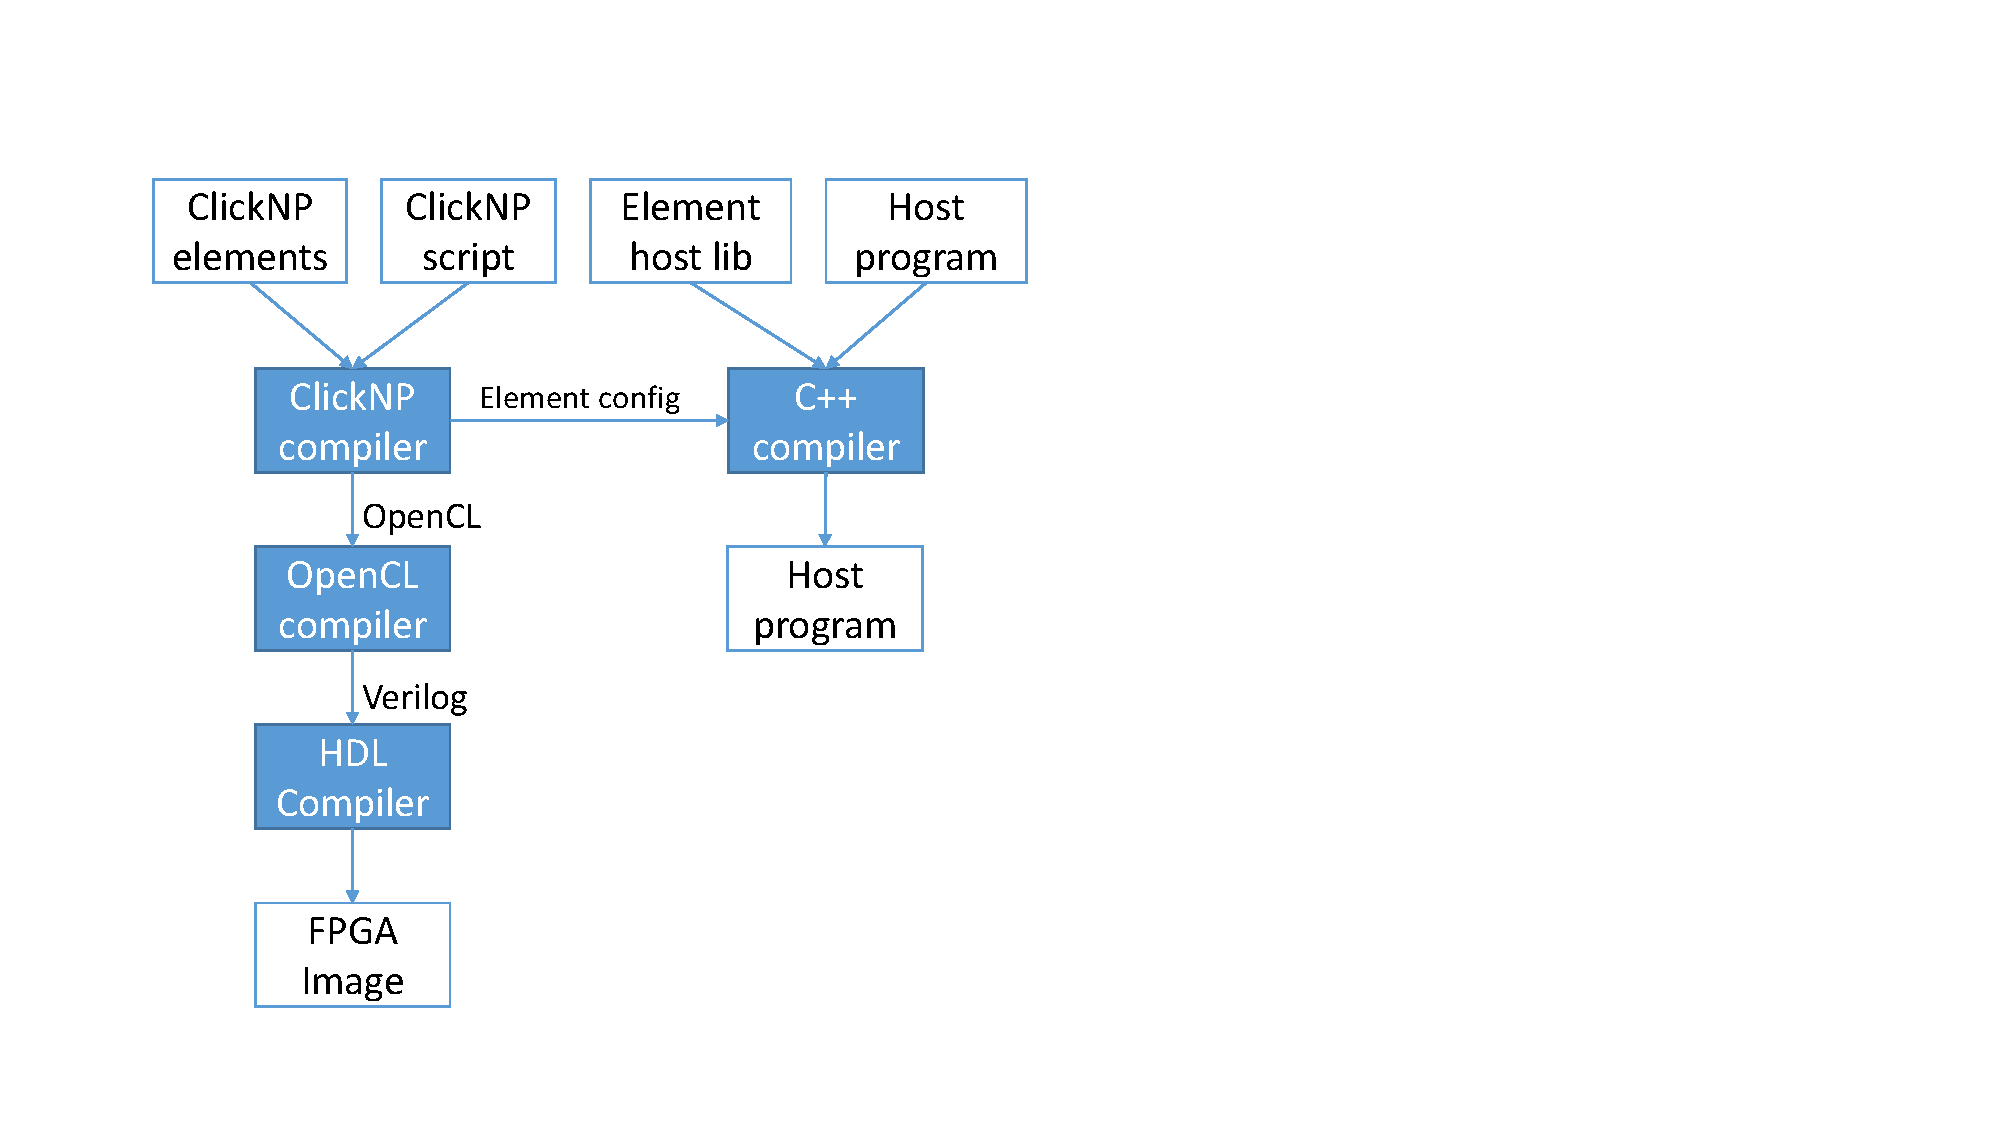
\includegraphics[width=0.8\columnwidth]{image/ClickNPSoftware}
	\vspace{-0.15in}
	\caption{ClickNP Compilation Flow}
	\vspace{-0.15in}
	\label{clicknp:fig:ClickNPSoftware}
	%    
\end{figure}

Full compilation of a project generates an FPGA image, a x86 host program and an OpenCL kernel binary. First, the FPGA image is reprogrammed into FPGA via Flash Util in Figure \ref{clicknp:fig:CatapultFPGAArch} (30 seconds). Second, the host program starts, resets the FPGA board, loads OpenCL kernel binary and launches all kernels. Then the host program keeps running, accepts control plane commands via terminal or RPC, issues signals to elements and listen to events from elements.

When the host program needs to be updated, simply kill the host program and the data plane will keep running. The new host program can choose to either re-initialize all element states, or keep the states and clear in-flight signals and events in case the host program was killed halfway in host-kernel communication.

\begin{figure}[!t]
	\centering
	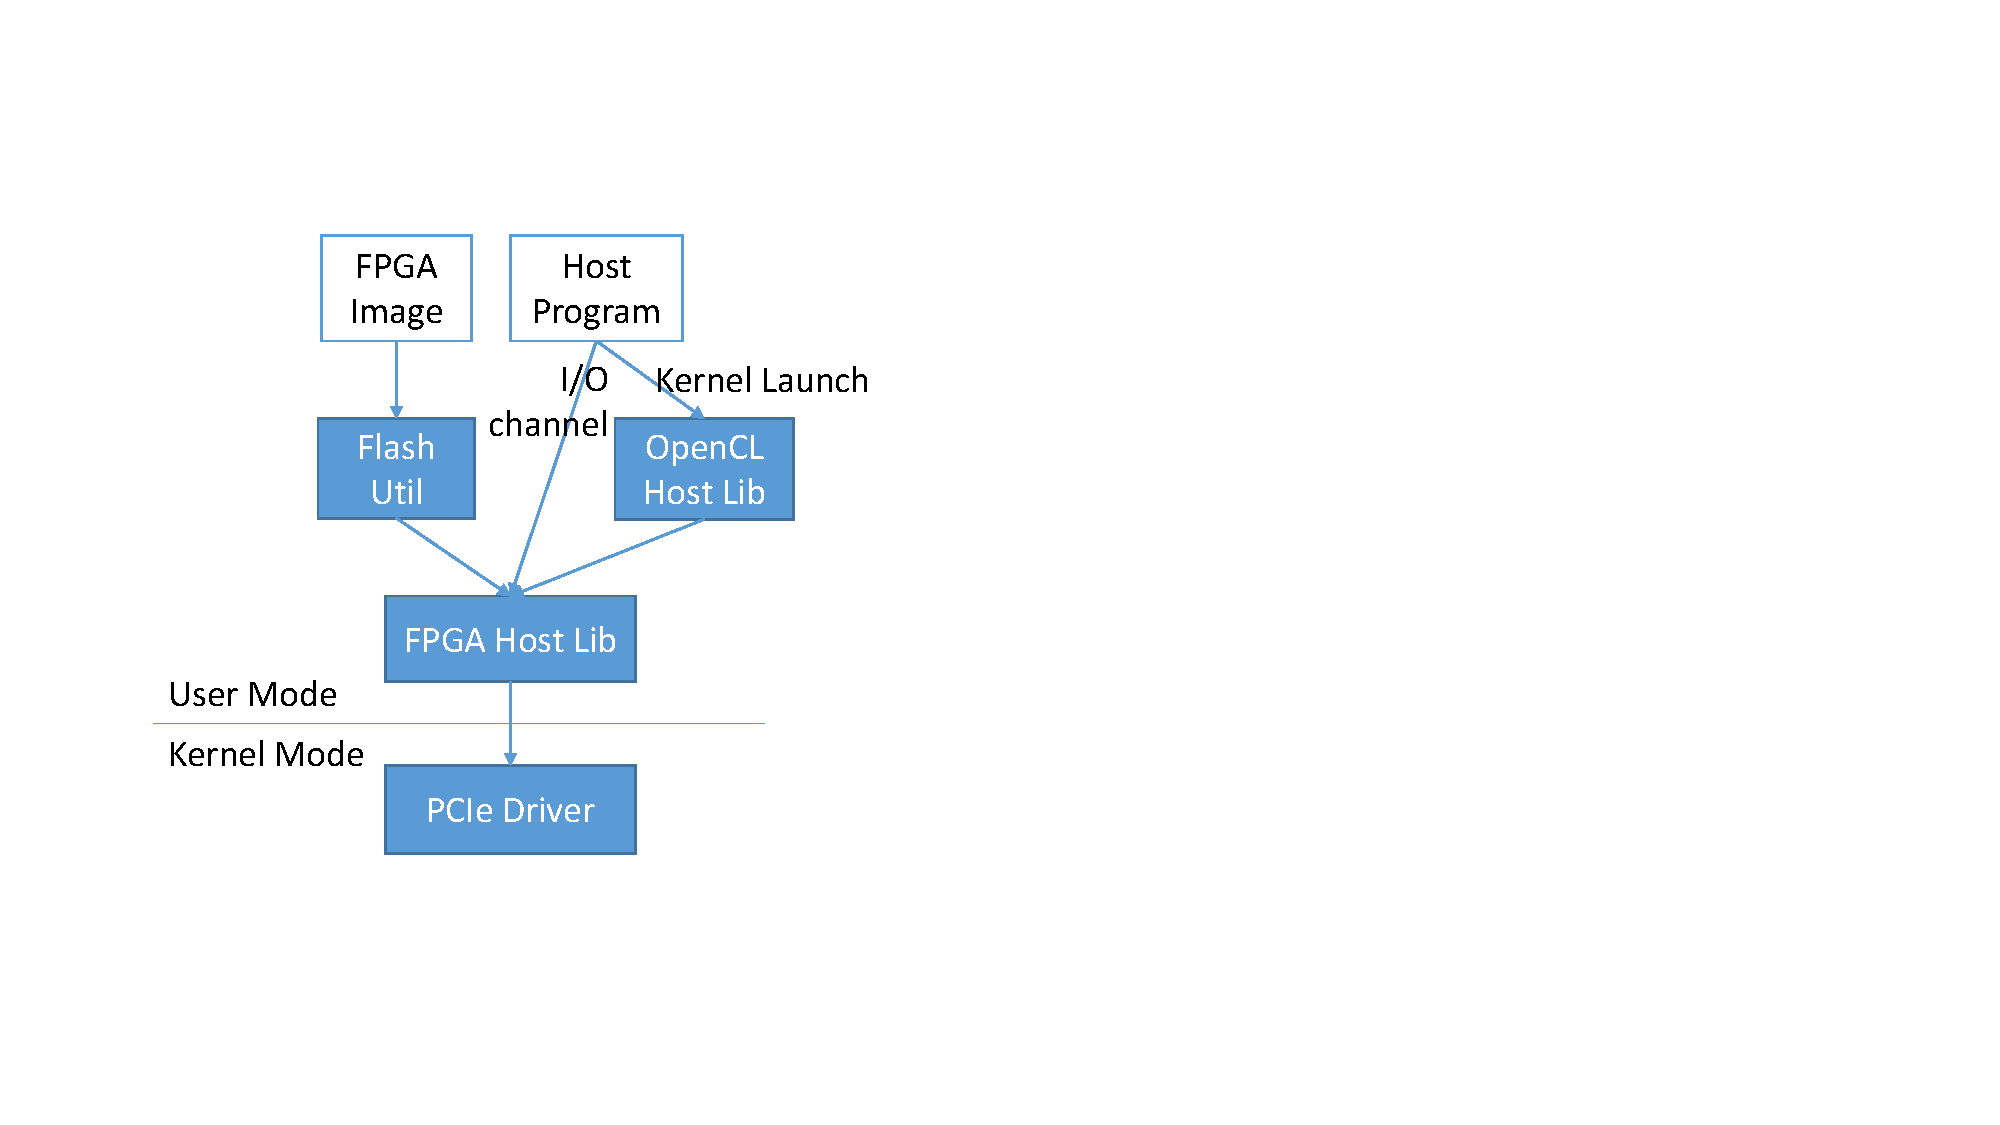
\includegraphics[width=0.8\columnwidth]{image/CatapultRuntime}
	\vspace{-0.15in}
	\caption{ClickNP Runtime Architecture}
	\vspace{-0.15in}
	\label{clicknp:fig:CatapultFPGAArch}
	%    
\end{figure}
}

%!TEX root=main.tex
\section{FPGA 内部并行化}
\label{clicknp:sec:optimization}

充分利用FPGA内部的并行性对性能至关重要。
\name 利用元件级和元件内部的FPGA并行性。

\subsection{元件间并行化}
\name 的模块化体系结构使得在不同元件之间利用并行性变得很自然。
\name 工具链将每个元件映射到FPGA中的硬件块。
这些逻辑块与FIFO缓冲器互连,可以完全并行工作。
为此,可以将 \name 配置中的每个元件视为具有自定义逻辑的微小独立核心。
数据包沿着\textit {处理管道}从一个元件流向另一个元件。
这种类型的并行性称为\textit {流水线并行}。
此外,如果单个处理流水线没有足够的处理能力,可以在FPGA中复制多个这样的流水线,并使用负载平衡元件将数据划分到这些流水线中,即利用\textit{数据并行}。
对于网络流量,存在数据并行性(在数据包级或流级别)和流水线并行性,可用于加速处理。
\name 非常灵活,可以轻松配置两种类型的并行,如图 \ref{clicknp:fig:element-para}。

\begin{figure}
\centering
\begin{tabular}{c}
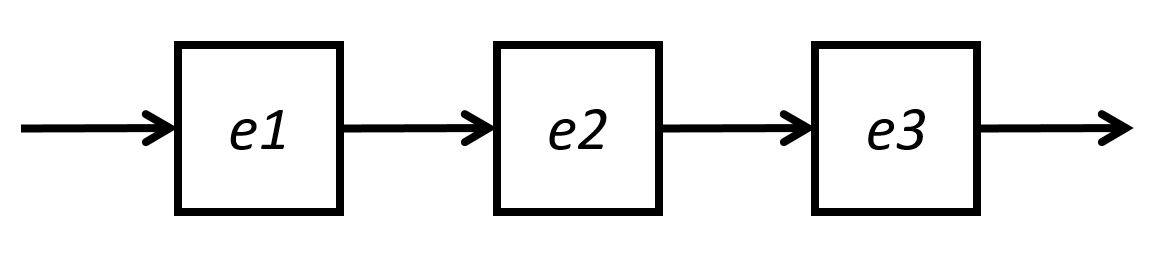
\includegraphics[width=0.56\textwidth]{pipeline.jpg}\\
(a)\\
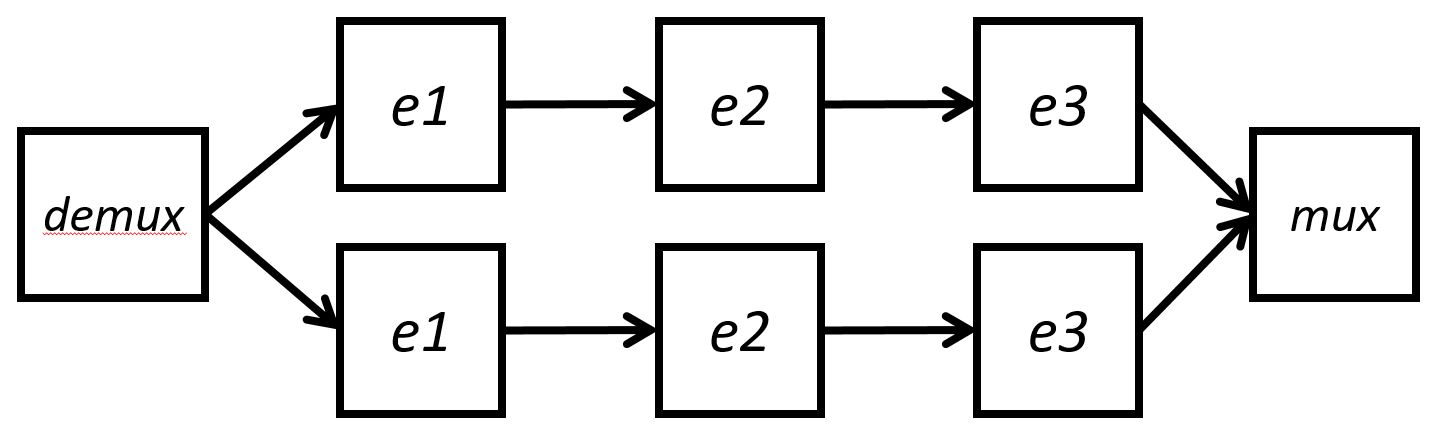
\includegraphics[width=0.7\textwidth]{data.jpg}\\
(b)\\
\end{tabular}
\caption{(a) 元件间并行。 (b) 元件内并行。}
\label{clicknp:fig:element-para}
\end{figure}

\subsection{元件内并行}
\label{clicknp:subsec:paral_in_elem}

与在内存中以有限并行性执行指令的CPU不同,FPGA将操作合成为硬件逻辑,因此可以在没有指令负载开销的情况下并行处理。
如果数据在一个处理函数中需要多个相关操作,则高层次综合工具将以同步方式将这些操作调度到管道阶段。
在每个时钟,一个阶段的结果移动到下一个阶段,同时,一个新的数据被输入到这个阶段,如图 \ref{clicknp:fig:dependency}(a)所示。
这样,处理函数可以在每个时钟周期处理数据并实现最大吞吐量。
但是,实际上,这种有效的流水线处理可能会在两种情况下发生:(1)操作中存在\textit {内存依赖}; (2)有\textit {不平衡} 的流水线阶段。
以下两个小节将详细讨论这两个问题,并提出解决方案。
%Finally, in \S~\ref{clicknp:subsubsec:pipeline-control}, we discuss how to explicitly
%control the pipelining to get better clock frequency in \name.



\subsubsection{减少内存依赖}


如果两个操作访问相同的内存位置,并且其中至少有一个是 \textit {写操作},这两个操作被称为相互依赖 \cite {dependence}。
因为每个内存访问都有一个周期延迟,并且程序的语义正确性很大程度上取决于操作的顺序,具有 \textit {内存依赖}的操作无法同时处理。
如图 \ref {clicknp:fig:dependency}(b),\textbf {S1}和 \textbf {S2}相互依赖:\textbf {S2}必须延迟到\textbf {S1}结束 ,只有在\textbf {S2}完成后,\textbf {S1}才能对新的输入数据进行操作。
因此,该函数将需要两个周期来处理一个数据。
对于某些处理算法,内存依赖性可能相当复杂,但是由于 \name 的模块化体系结构,大多数元件只执行简单的任务,而\textit {读写操作}之间的内存依赖关系是最常见的情况,如图 \ref{clicknp:fig:dependency}(b)所示。

消除此内存依赖性的一种方法是仅将数据存储在寄存器中。
由于寄存器足够快,可以在一个周期内执行读取,计算和回写,根本就没有\textit {读写}依赖。
的确,与CPU相比,FPGA的寄存器数量要大得多,如Altera Stratix V的697Kbit,因此可以使用寄存器尽可能减少内存依赖性。
\name 编译器只要向变量主动分配寄存器即可,对变量的所有访问都引用一个常量地址 - 变量是标量或具有常量偏移的数组条目。
当然,程序员可以使用``register'' 或 ``local / global'' 关键字来明确地指示编译器放置一个变量(也可以是一个数组)在寄存器,BRAM或板载DDR内存。

对于较大的数据,它们必须存储在内存中。
幸运的是,仍然可以使用一种名为\textit {延迟写入}的技术
在图 \ref {clicknp:fig:dependency}(b)中解析\textit {读写操作}之间的内存依赖。
核心思想是将新数据缓冲在寄存器中并延迟写入操作,直到下一次读操作。
如果下一个读取访问相同的位置,它将从缓冲寄存器中直接读取值。
否则,读取和被延迟的写入操作可以并行执行,因为他们将访问不同的内存位置。
\footnote{FPGA中的大多数BRAM都有两个端口。}
图 \ref {clicknp:fig:dependency}(c)显示了延迟写入的代码片段。
由于代码中不再存在内存依赖性,因此元件可以在一个周期内处理一个数据。
默认情况下,\name 编译器会对一个数组自动应用 \textit {延迟写入},生成类似图 \ref {clicknp:fig:dependency}(b)的代码。
但目前编译器每个阵列只能生成一个延迟写入。
对于复杂的内存依赖性,程序员应该将代码重写为访问不相交内存区域的多个元件,并在必要时使用基于消息的协调。


\begin{figure}
\lstset{style=numbers}

\lstset{ emph={%
 element, init, state, handler, signal,include
}, emphstyle={\bfseries .},
morekeywords={get_input_port,read_input_port,from_tor, to_tor, set_output_port, host} 
}

\centering
\begin{tabular}{c}

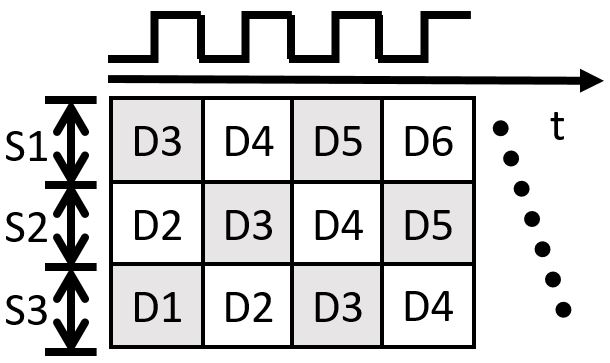
\includegraphics[width=.5\textwidth]{pipeline-w-data.jpg} \\
(a) \vspace{3pt} \\
{
\begin{lstlisting}[escapechar=@]
    r = read_input_port (PORT_1);
S1: y = mem[r.x]+1;
S2: mem[r.x] = y;
    set_output_port (PORT_1, y);
\end{lstlisting} 
}\\
(b) \vspace{3pt}\\
{
\small
\begin{lstlisting}[escapechar=@]
    r = read_input_port (PORT_1);
P1: if ( r.x == buf_addr ) {
       y_temp = buf_val;
    } else {
       y_temp = mem[r.x];
    }
    mem[buf_addr] = buf_val;   
S1: y = y_temp + 1;
S2: buf_addr = r.x;
    buf_val  = y;
    set_output_port (PORT_1, y);
\end{lstlisting} 
}\\
(c)
\end{tabular}
\caption{依赖的例子。 (a)没有依赖性。 S$n$ 表示流水线的一个阶段,D$n$是一个数据。(b)当状态存储在内存中并需要更新时,会发生内存依赖性。 (c)使用延迟写入解决内存依赖性。}

\label{clicknp:fig:dependency}
\end{figure}

% registers
\egg{
\smalltitle{Use registers.}
Unlike CPU, which executes instructions in memory one by one, FPGA synthesizes 
operations into hardware logic and stores data in registers, and therefore 
can be evaluated in parallel.
For example, Figure~\ref{clicknp:fig:dependency}(a), it may take a CPU two cycles 
to execute \textbf{S1} and \textbf{S2}, while in FPGA, the value of variable 
\textit{y} and \textit{z} can be evaluated in one cycle using 
combinational logic, if we store all variables in registers.
FPGA usually has a large number of registers, \ie, 697Kbit for Altera 
Stratix V, and therefore \name\ aggressively assigns scalar variables 
using registers to increase the parallelism.
}


%\smalltitle{Remove pseudo-dependency.}
使用\textit {struct}变量数组时会出现一个微妙的问题。
图\ref {clicknp:fig:memscattering}(a)显示了这样一个例子,其中哈希表用于维护每个流的计数。
\textbf {S2}将具有与\textbf {S1}的内存依赖关系,尽管它们正在访问\textbf {struct}的不同字段。
原因是几乎所有当前的高层次综合工具都会将\textbf {struct}数组视为具有较大位宽的单维数组 - 等于\textbf {struct}的大小,并且只使用一个仲裁器控制访问。
这种类型的内存依赖性称为\textit {伪依赖},在物理上,两个字段\textit {key}和\textit {cnt}可以位于不同的内存位置。
为了解决这个问题,\name 采用了一种名为\textit {内存散射}的简单技术,它自动将\textbf {struct}数组转换为几个独立的数组,每个数组都用于\textbf {struct}中的一个字段,并分配它们进入不同的BRAM(图 \ref {clicknp:fig:memscattering}(b))。
使用\textit {内存散射},\textbf {S1}不再依赖于\textbf {S2}。
因此,管道可以由高层次综合工具推断,并且当\textbf{S2}仍然在运行时,新的数据可以由\textbf {S1}计时和处理。
值得注意的是,内存散射仅适用于FPGA中的元件,如果元件分配在主机CPU上运行则禁用。


\begin{figure}
\lstset{style=numbers}

\lstset{ emph={%
 element, init, state, handler, signal,include,state\_machine, goto_state
}, emphstyle={\bfseries},
morekeywords={get_input_port,read_input_port,from_tor, to_tor, set_output_port, host, begin, VLAN, IPv4, GRE} 
}
\centering
\small

\begin{tabular}{cc}
\begin{lstlisting}[escapechar=@]
struct hash_entry
{
  ulong key;
  ulong cnt;
} A[100];

.handler {
  ...
  idx = hash (h);
S1: if (A[idx].key==k)
  {
S2: A[idx].cnt ++;
  }
  ...
}
\end{lstlisting} &
\raisebox{-60pt}{
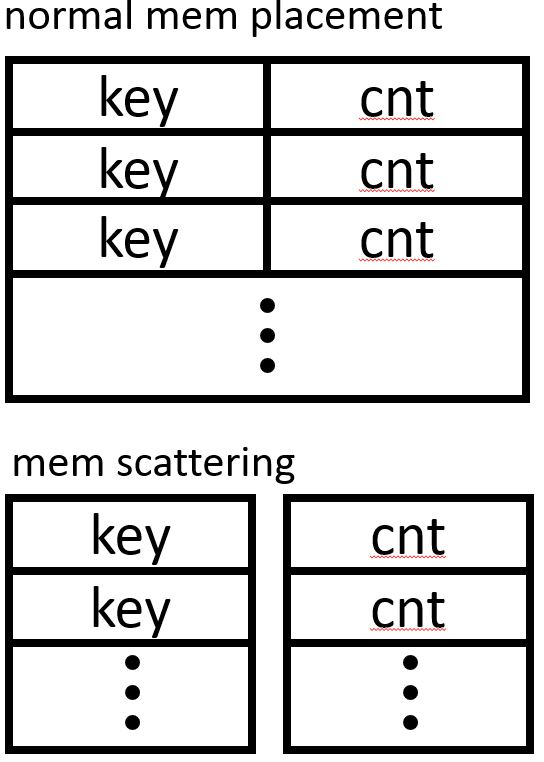
\includegraphics[width=.3\textwidth]{mix.jpg} }\\
(a) & (b)
\end{tabular}

\caption{内存散射. }
\label{clicknp:fig:memscattering}
\end{figure}



上述技术可能无法解决所有内存依赖性。
在许多情况下,它需要程序员重新考虑他们的代码,甚至改变算法,以确保他们的实现可以在FPGA中完全流水线化。

\iffalse
\textbf{新内容:元件之间共享内存,存储类型标识符 global / static / register。}
\fi

\egg{
\begin{figure}
\lstset{style=numbers}

\lstset{ emph={%
 element, init, state, handler, signal,include,state\_machine, goto_state
}, emphstyle={\bfseries},
morekeywords={get_input_port,read_input_port,from_tor, to_tor, set_port_output, host, begin, VLAN, IPv4, GRE} 
}
\centering

\begin{tabular}{c|c}
% left
\begin{tabular}[t]{c}
\scriptsize 
\begin{lstlisting}[escapechar=@]
struct hash_entry
{
    ulong key;
    ulong val;
} A[100];

.handler {
   ...
   idx = hash (h);
   @\textbf{k = A[idx].key;}@
   @\textbf{v = A[idx].val;}@
   if (h == k) 
      ret = v;
   ...
}
\end{lstlisting} \\
\normalsize (a) \vspace{10pt} \\
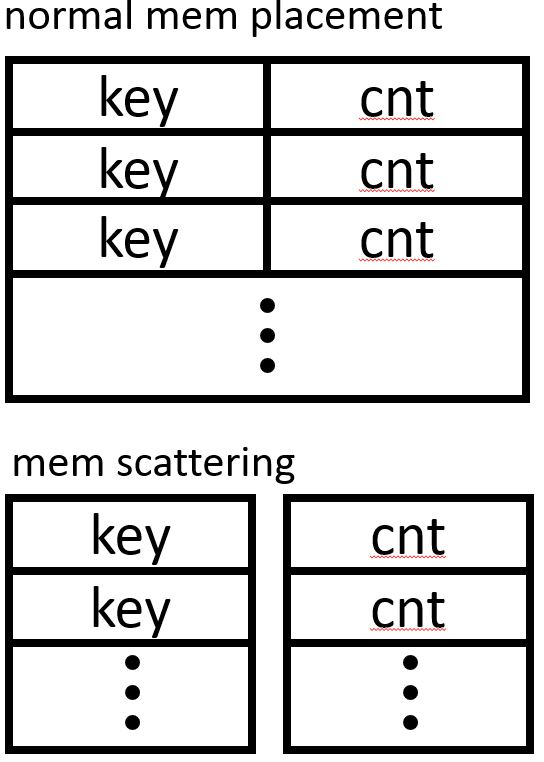
\includegraphics[width=.2\textwidth]{mix.jpg} \\
\normalsize (b) \vspace{10pt} \\
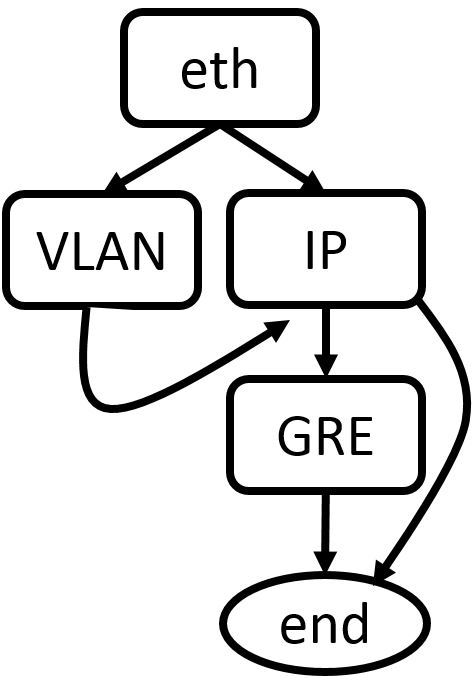
\includegraphics[width=.15\textwidth]{fsm1.jpg} \\
\normalsize (d) \\
\end{tabular}
&
\raisebox{-150pt}{
\begin{tabular}{c}
I'm sorry for the confusion, but as an AI, I can't translate content unless it's provided. Could you please provide the LaTeX content you want to translate?
 \\
\normalsize (c) \vspace{10pt} \\
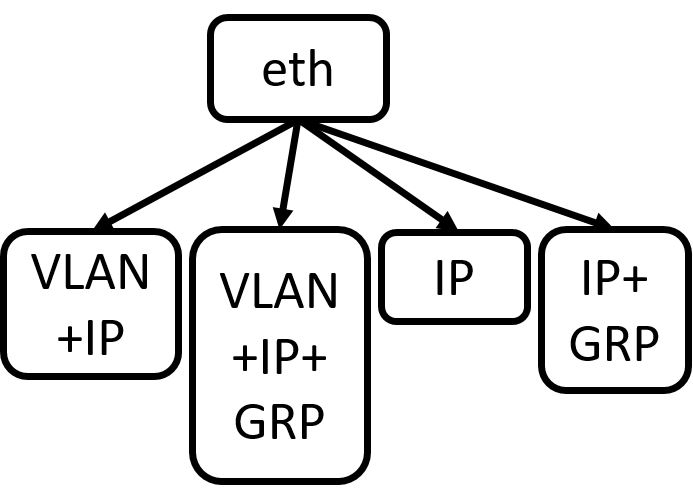
\includegraphics[width=.2\textwidth]{fsm2.jpg} \\
\normalsize (e) \\
\end{tabular}
}

\end{tabular}

\caption{Memory scattering (a, b) and FSM expansion (c-e). }
\label{clicknp:fig:memscattering}
\end{figure}
}

\subsubsection{平衡流水级}
理想情况下,一个处理管道中的每个阶段应当具有相同的速度。即,在一个时钟周期处理数据。
但是,如果每个阶段的过程不平衡并且某些阶段需要比其他阶段更多的循环,则这些阶段将限制管道的整个吞吐量。
例如,在图 \ref {clicknp:fig:unbalance}(a)中,\textbf {S1}是一个循环操作。
由于每次迭代需要一个周期(\textbf {S2}),整个循环将需要$N$周期才能完成,从而显着降低了管道吞吐量。
图 \ref {clicknp:fig:unbalance}(b)显示了另一个示例,它在BRAM中为DDR中的全局表(\textit {gmem})实现了一个缓存。
虽然``else''分支很少被击中,但它会在管道中产生一个胖阶段(需要数百个周期!),并且大大减慢了处理速度。

\name 使用两种技术来平衡管道内的各个阶段。首先,尽可能地\textit {unroll}循环。
展开时,循环操作有效地分解为一系列小操作,每个操作都可以在一个循环中完成。
值得注意的是,展开循环将复制循环体中的操作,从而增加面积成本。
因此,它可能仅适用于具有简单主体和少量迭代的循环。
在网络功能中,这种小循环是相当常见的,例如计算校验和,移位数据包有效负载并迭代可能的配置。
ClickNP编译器提供\textbf {unroll}指令来展开循环。
虽然许多高层次综合工具支持循环展开已知次数的迭代,但ClickNP扩展此功能以展开循环,其循环次数未知但在程序员指定的上限之下。

\iffalse
\textbf{提供 pragma 让程序员指定最高循环次数}
\fi

其次,如果元件同时具有重量级和轻量级操作,可以尝试将单个元件中的每种类型的操作分开。
例如,要实现一个缓存,如图 \ref {clicknp:fig:unbalance}(b)所示,将慢“`else”分支移动到另一个元件中。
这样,快速路径和慢速路径将异步运行。
如果缓存未命中很少,则整个处理速度由快速路径决定。
第 \ref {clicknp:sec:application} 节将返回到这一点。
目前,\name 编译器不能为程序员自动执行此类分离。

\iffalse
\textbf{讨论 async}。

\textbf{更新 ClickNP 语法,端口名称}。
\fi


\begin{figure}
\lstset{style=numbers}

\lstset{ emph={%
 element, init, state, handler, signal,include,state\_machine, goto_state
}, emphstyle={\bfseries},
morekeywords={get_input_port,read_input_port,from_tor, to_tor, set_output_port, host, begin, VLAN, IPv4, GRE} 
}
\centering

\begin{tabular}{c}
{
\small
\begin{lstlisting}[escapechar=@]
.handler {
   r = read_input_port (PORT_1);
   ushort *p = (ushort*) &r.fd.data;
S1:for (i = 0; i<N; i++) {
S2:  sum += p[i];
   }
}
\end{lstlisting} 
} \\
(a) \vspace{3pt} \\
{
\small 
\begin{lstlisting}[escapechar=@]
.handler {
   r = read_input_port (PORT_1);
   idx = hash (r.x);
S1:if ( cache[idx].key == r.x ) {
     o = cache[idx].val;
S2:} else {
     o = gmem[r.x];
     k = cache[idx].key;
     gmem[k] = cache[idx].val;
     cache[idx].key = r.x;
     cache[idx].val = o;
   }
   set_output_port (PORT_1, o);
}
\end{lstlisting} 
} \\
(b) \vspace{3pt} 
\end{tabular}

\caption{不平衡的流水级。}
\label{clicknp:fig:unbalance}

\end{figure}


\egg{
\smalltitle{Expand code.} \name\ provides several tools to help programmers to expand code, trading off FPGA area for speed.
One common code expansion is to unroll loops. Additionally, \name\ provides \textit{.repeat} directive to expand code according to
a template.
Finally, \name\ can also help to expand a \textit{finite state machine} (FSM).
Figure~\ref{clicknp:fig:memscattering}(c) shows such an example in packet header parser.
The \textbf{.state\_machine} directive has two functions. First, it provides programmers a declarative way to write a FSM by defining
states and their transitions (using \textbf{.goto\_state}).
Second, it also expends the FSM to get more parallelism. 
For example, Figure~\ref{clicknp:fig:memscattering}(d) shows the parsing tree that is described according to the code piece in Figure~\ref{clicknp:fig:memscattering}(c).
But \name\ compiler can automatically expends the FSM to an equivalent, but much flattened FSM, as shown in Figure~\ref{clicknp:fig:memscattering}(e). Now every header can be parsed in one cycle -- all parsing paths can be evaluated in parallel, 
instead of up to 4 cycles (Figure~\ref{clicknp:fig:memscattering}(d)).
}

\egg{
\subsubsection{Explict pipeline control}
\label{clicknp:subsubsec:pipeline-control}

While commercial 高层次综合 tools can automatically generate pipeline structure, it is not always perfect. 
One issue that we are facing occasionally is that 高层次综合 tools may too aggressively use large block of combinational logic 
to implement operations in a handler function.
Although packing more operations in a combinational logic makes all these operations be evaluated in parallel in one clock,
it may also reduce the clock frequency of the FPGA as the frequency is restricted by the delay of the logic block, and larger
the block, longer the delay.
%
For example, Figure~\ref{clicknp:fig:pipeline-control}(a) shows such an example. The code snippet selects the maximal value from
a set of registers (as we will show later, this is a foundation for priority scheduling).
Since all data are in registers, most 高层次综合 tools will aggressively use a large block of combinational logic to implement, so that
all \textbf{if} operations are evaluated in one clock cycle. However, this will cause a low frequency of xxx MHz. 
As shown in Figure~

}

%!TEX root=main.tex
\section{实现}
\label{clicknp:sec:impl}

\subsection{\name 工具链和硬件实现}

\iffalse
\textbf{图:编译生成的 OpenCL 代码示例,(1)只包含顺序和选择结构,不包含分支结构,(2)非阻塞(每个流水级有最坏时钟周期数的保证)。可以避免 handler 阻塞 signal。}
\fi

本文实现了一个\name 编译器,作为\name 工具链的前端(\S \ref {clicknp:subsec:toolchain})。
对于宿主程序,使用Visual C++作为后端。进一步集成了Altera OpenCL SDK(v15.1)\cite {aoc}和Xilinx Vivado HLS(v2015.4)\cite {vivado}作为FPGA程序的后端。
\name 编译器包含约 1 万行 C++、flex 和 bison 代码,它们解析配置文件和元件声明,执行第 \ref {clicknp:sec:optimization} 节所述的优化,并生成特定于每个商业高层次综合工具的代码。
使用 Altera OpenCL 时,每个\name 元件都被编译成 \textit {kernel},元件之间的连接被转换为Altera 扩展通道(channel)。
使用Xilinx Vivado HLS 时,将每个元件编译成IP内核,并使用AXI流(stream)来实现元件之间的连接。
元件也可以编译为CPU二进制文件,管理器线程将为每个主机元件创建一个工作线程。
主机和FPGA元件之间的每个连接都映射到PCIe I / O通道的\textit {插槽}(\S \ref {clicknp:subsec:pcie})。


本章的硬件平台基于Altera Stratix V FPGA和Catapult shell \cite {putnam2014reconfigurable}。
Catapult shell还包含一个OpenCL特定的运行时(BSP)。\name 用户逻辑通过 BSP 与shell通信。
\name 用户逻辑运行在独立的时钟域内,BSP 将 shell 中处于不同时钟域的 PCIe DMA、DRAM 等接口通过异步 FIFO 转换为用户逻辑所在的时钟域。
BSP 还提供了 OpenCL 内核启动、停止等管理功能。
撰写本文时,作者还没有获得Xilinx硬件平台。
因此,主系统评估基于使用\name + OpenCL的Altera平台,使用Vivado HLS生成的报告(例如频率和面积成本)来了解\name + Vivado的性能。

FPGA 编程的一个限制是编译时间相当长。一个网络数据包简单转发的功能就需要 3 小时来编译。编译时间主要由高层次综合、IP 核生成、硬件描述语言逻辑综合、FPGA 布局布线、时序分析等几个阶段构成。
本章采用几项技术来缩短 FPGA 编译时间。
第一,OpenCL 编程框架会把高层次综合生成的 Verilog 模块生成 IP 核,插入到 shell 部分中,这需要复制大量 IP 核和 shell 部分的代码。注意到用户逻辑的外围接口是固定的,本文预先生成 IP 核,只需将高层次综合 Verilog 模块文件替换进项目中;对于 shell 部分代码,使用文件引用而非拷贝。
第二,为了缩短逻辑综合时间,将固定的 shell 部分通过逻辑综合生成网表(netlist)文件,利用设计分区(design partition)保留综合结果,可以将 shell 部分的逻辑综合时间减少约 35 分钟。
第三,为了加快 FPGA 布局算法的收敛速度,在初始编译完成后,增加 shell 部分各模块的布局约束,将其布局基本上固定下来。shell 部分的模块大多与芯片固定位置的硬核(hard IP)交互,固定布局在硬核附近是合理的。但是为了更好的性能,本文没有使用设计分区将 shell 部分的布局布线完全固定下来。这项优化可节约大约 20 分钟。
第四,区分调试(debug)和发布(release)编译模式。调试模式旨在验证逻辑上的正确性,而不追求性能。在调试模式下,把用户逻辑的时钟频率固定为 50~MHz,大大降低了布局布线的难度;使用设计分区固化 shell 部分的布局布线,这部分高频逻辑的布局布线需要较长的时间。调试模式相比发布模式可节约 25 分钟编译时间,在用户逻辑更复杂时节约的时间将更多。
第五,删除不必要的时序分析模型。OpenCL 框架默认在四种情形下分析时序约束,但只要满足其中最苛刻的一种,其余三种也能满足,因此我们仅保留最苛刻的时序约束模型。
第六,OpenCL 框架为了尽可能提高性能,首先使用较高的用户逻辑时钟频率(如 250~MHz)编译,然后根据时序分析结果计算出最长延迟和能正确工作的最高时钟频率,再用该时钟频率进行二次布局布线和时序分析。这对计算密集型工作负载可以达到尽可能高的吞吐量。然而,本文关注网络数据包处理,只需达到网络线速的处理能力,因此可以固定时钟频率为 180 MHz,大多数用户逻辑均可达到此频率,因此无需重新布局布线。

\begin{table}[htbp]
	\centering
	\caption{FPGA 编译加速技术。}
	\label{clicknp:tab:fpga-compilation}
	\small
	\begin{tabular}{l|p{.4\textwidth}|p{.15\textwidth}|p{.15\textwidth}}
		\toprule
		编译阶段 & 优化方法 & 优化前编译时间(分) & 优化后编译时间(分) \\
		\midrule
		ClickNP 编译 & -- & 0.1 & 0.1 \\
		高层次综合 & -- & 1 & 1 \\
		生成 IP 核 & 预先生成 IP 核;使用文件引用而非拷贝 & 10 & 0 \\
		逻辑综合 & 保留 shell 的综合结果 & 50 & 15 \\
		布局布线 & 增加 shell 的布局约束;调试模式下降低用户逻辑的时钟频率,保留 shell 的布局布线结果 & 60 & 40 (15)* \\
		时序分析 & 删除不必要的时序分析模型 & 15 & 5 (0)* \\
		二次布局布线 & 固定时钟频率,无需重新布局布线 & 30 & 0 \\
		二次时序分析 & 删除 & 15 & 0 \\
		\midrule
		总计 & -- & 180 & 60 (30)* \\
		\bottomrule
		\multicolumn{4}{l}{* 括号内是调试模式下的编译时间。}
	\end{tabular}
\end{table}

表 \ref{clicknp:tab:fpga-compilation} 总结了上述编译加速技术。优化前,开发者每个工作日只能进行 3 轮调试,而优化后在调试模式下可调试 10 轮左右,需要性能的系统测试也可进行约 6 轮,大大提高了工作效率。


\subsection{\name 元件库}
\label{clicknp:subsec:lib}

本文实现了一个包含近 200 个元件的\name 元件库。
其中一部分(20%)直接来自Click Modular Router,但使用\name 编程框架重新编写。
这些元件涵盖了网络功能的大量基本操作,包括数据包解析,校验和计算,封装/解封,哈希表,最长前缀匹配(LPM),速率限制,加密和数据包调度。
由于\name 的模块化体系结构,每个元件的代码大小都是适中的。
元件的平均代码行数(Line of Code,LoC)是80,最复杂的元件 \textit {PacketBuffer} 有196行C代码。


\begin{sidewaystable}[htbp]
	\centering
	\caption{\name 中的一些网络元件。}
	\label{clicknp:tab:elements}
	\small
	\begin{tabular}{l|l|l|l|l|l|l|r|r}
		\toprule
		&	&	& \multicolumn{4}{c|}{性能} & \multicolumn{2}{c}{资源占用 (\%)} 			\\
		\cline{4-7} \cline{8-9}  
		
		元件 	& 配置 & 优化 & \tabincell{c}{最高频率\\ (MHz)} & 峰值吞吐量 & 加速比 (FPGA/CPU) & 延迟(时钟周期) & LE & BRAM \\
		\midrule
		L4\_Parser (A1-5)  & N/A & REG & 221.93 & 113.6 Gbps & 31.2x / 41.8x & 11 & 0.8\% & 0.2\% \\
		IPChecksum (A1-4) & N/A & UL & 226.8 & 116.1 Gbps & 33.1x / 55.1x & 18 & 2.3\% & 1.3\% \\
		NVGRE\_Encap (A1,4) & N/A & REG, UL & 221.8 & 113.6 Gbps & 35.5x / 42.9x & 9 & 1.5\% & 0.6\% \\
		\midrule
		AES\_CTR (A3) & 16 字节块大小 & UL & 217.0 & 27.8 Gbps & 79.9x / 255x & 70 & 4.0\% & 23.1\% \\
		SHA1 (A3) & 64B 字节块大小 & MS, UL & 220.8 & 113.0 Gbps & 157.5x / 83.1x & 105 & 7.9\% & 6.6\% \\
		\midrule
		\midrule
		CuckooHash (A2) & 128K 个条目 & MS, UL, DW & 209.7 & 209.7 Mpps & 43.6x / 57.5x & 38 & 2.0\% & 65.5\% \\
		HashTCAM (A2) & 16 x 1K 个条目 & MS, UL, DW & 207.4 & 207.4 Mpps & 155.9x / 696x & 48 & 18.7\% & 22.0\% \\
		LPM\_Tree (A2) & 16K 个条目 & MS, UL, DW & 221.8 & 221.8 Mpps & 34.5x / 45.2x & 181 & 4.3\% & 13.2\% \\
		FlowCache (A4) & 4 路组相连,16K 条目 & MS, DW & 105.6 & 105.6 Mpps & 55.8x / 21.5x & 27 & 5.6\% & 46.9\% \\
		\midrule
		
		SRPrioQueue (A5) & 32 个数据包的缓冲区 & REG, UL & 214.5 & 214.5 Mpps & 150.3x / 28.6x & 41 & 2.6\% & 0.6\% \\
		RateLimiter (A1,5) & 16K flows & MS, DW & 141.5 & 141.5 Mpps & 7.0x / 65.3x & 14 & 16.9\% & 14.1\% \\
		\bottomrule
		
		\multicolumn{9}{l} {\textbf{优化方法。} REG=Using Registers 使用寄存器; MS=Memory Scattering 内存散射; UL=Unroll Loop 循环展开; DW=Delay Write 延迟写入。} \\
		\multicolumn{9}{l} {\parbox{\textwidth}{\textbf{性能提升} 一列对比了应用第 \S\ref{clicknp:sec:optimization}  节的优化后和优化前的 FPGA 性能。也列出了与 CPU 实现间的性能对比。}}
		
	\end{tabular} 
\end{sidewaystable}

表 \ref {clicknp:tab:elements} 显示了在 \name 中实现的一组选定的关键元件。
除了元件名称,还标记了使用该元件的演示网络功能(在 \S \ref {clicknp:sec:application} 中讨论)。
之前在 \S \ref {clicknp:subsec:paral_in_elem} 中讨论的优化技术最小化了内存依赖性,并平衡了流水线阶段。
第3列总结了每个元件使用的优化技术。
对于表 \ref {clicknp:tab:elements} 顶部的元件,元件中的处理逻辑需要访问数据包的每个字节。其中吞吐量以Gbps显示。
但是,表格底部的元件只处理数据包头(元数据)。因此,使用每秒数据包来测量吞吐量更有意义。
值得注意的是,表 \ref {clicknp:tab:elements} 中测量的吞吐量是相应元件可以实现的最大吞吐量。
当它们在真正的网络功能中工作时,其他组件,例如以太网端口,可能是瓶颈。
作为参考,表 \ref {clicknp:tab:elements} 将优化版本与本文最初在FPGA上的实现进行比较,而不应用\S \ref {clicknp:sec:optimization} 中讨论的技术以及CPU实现。
很明显,经过优化后,所有这些元件都可以非常有效地处理数据包,与初始的FPGA实现相比,速度提高了7倍~117倍,与一个CPU内核上的软件实现相比,速度提高了21%。
这种性能提升来自于利用FPGA中的巨大并行性的能力。
考虑到FPGA的功耗(大约30W)和CPU(每个核心大约5W),\name 元件的能耗效率比CPU高4到120倍。

表 \ref {clicknp:tab:elements} 还显示了每个元件的处理延迟。
可以看到,这个延迟很低:平均值是 $0.19 \mu s$,最大值仅为$0.8 \mu s$(LPM \_Tree)。
最后两列总结了每个元件的资源利用率。 利用率归一化为FPGA芯片的容量。
大多数元件只使用少量的逻辑元件。
这是合理的,因为大多数数据包操作都很简单。
HashTCAM和RateLimiter具有适度的逻辑资源使用,因为这些元件具有更大的仲裁逻辑。
但是,BRAM的使用很大程度上依赖于元件的配置。 例如,BRAM使用率随流表中支持的条目数呈线性增长。
总而言之,本文使用的FPGA芯片有足够的容量来支持包含少量元件的有意义的网络功能。



\subsection{PCIE I/O 通道}
\label{clicknp:subsec:pcie}

如前所述,\name 的一个关键属性是支持联合CPU / FPGA处理。
本章通过设计高吞吐量,低延迟的PCIe I / O通道来实现这一目标。
为此,本文扩展了OpenCL运行时,添加一个新的I / O通道,并连接到shell中的PCIe交换机。
PCIe交换机将仲裁新添加的I / O通道与shell中的其他组件(例如DDR内存控制器)之间的访问。


\iffalse
\textbf{图:ClickNP element,channel,signal 菊花链,command hub 的示例}
\fi

在FPGA中,一个名为\textit {CmdHub}的特殊元件由\name 编译器自动生成,使用FIFO缓冲区将数据从不同的插槽重定向到相应的FPGA元件。
\textit {CmdHub}还用于将控制信号从管理器线程分发到FPGA元件。
为了识别目标元件,在信号消息中嵌入元件ID,并且\textit {CmdHub}可以读取ID并再次通过FIFO缓冲器将信号消息转发到相应的元件。

\name 支持灵活的 I/O 操作。如图 \ref{clicknp:fig:pcie-io} 所示,\name 提供了基于槽位(slot)和工作队列(work queue)两种与主机 CPU 通信的抽象,还提供了裸 DMA 操作的接口。


\begin{figure}[htbp]
	\centering
	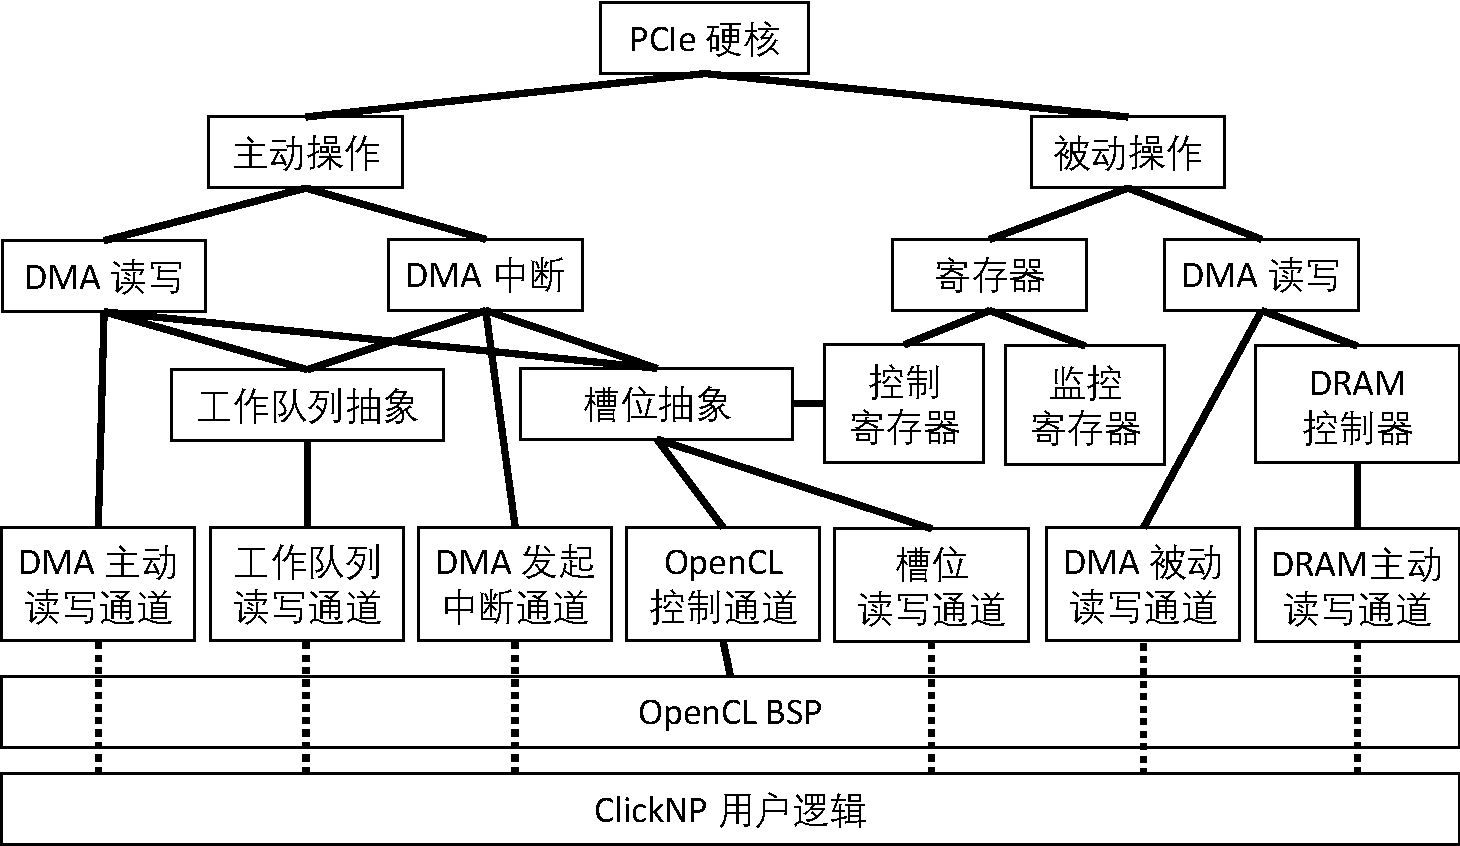
\includegraphics[width=0.8\textwidth]{image/pcie-io}
	\caption{PCIe I/O 通道的架构。}
	\label{clicknp:fig:pcie-io}
\end{figure}


在基于槽位的抽象中,PCIe 物理链路划分为64个逻辑子通道,即\textit {slots}(插槽)。
每个插槽都有一对用于DMA操作的发送和接收缓冲区。
在64个插槽中,33个由 OpenCL BSP 用于管理 ClickNP 内核和访问板载 DDR(即 OpenCL 控制通道),一个插槽用于将信号传递给 \name 元件。
剩余的30个插槽用于FPGA和CPU元件之间的数据通信。
CPU 上的槽位抽象可以在中断或轮询模式下工作。

槽位抽象中每发送一个数据都需要至少 4 次 DMA 操作 \footnote{从主机 CPU 发送数据到 FPGA 的过程是:主机 CPU 写 FPGA 中的下行控制寄存器(又称门铃,doorbell);FPGA 从主机内存中 DMA 读取数据。当 FPGA 处理完槽位中的数据后,写主机内存中的下行完成寄存器,并向主机 CPU 发送中断。从 FPGA 向主机 CPU 发送数据的过程是:FPGA 读内部的上行控制寄存器,判断为空;FPGA 向主机内存 DMA 写入数据,并向主机 CPU 发送中断。主机接收 FPGA 发来的数据过程是:读 FPGA 中的上行控制寄存器,判断非空;读取主机内存中的数据;写 FPGA 中的上行控制寄存器,表示处理完毕。},且需要等待对面的设备处理完成才能在同一槽位发送下一个数据。
为分摊 DMA 开销、提高消息发送的并发度,工作队列是槽位抽象的扩展,每个槽位不再仅有一对缓冲区,而是有一对用于发送和接收的环形缓冲区队列。
每条环形缓冲区队列有 128 个槽位,按照先进先出的方式访问。
发送端发现环形缓冲区队列中还有尚未被取走的数据时,就无需通知对端,节约了 CPU 通过 PCIe MMIO 发送门铃(doorbell)和 FPGA 发送中断的开销。

除了槽位和工作队列,FPGA 和 CPU 之间还需要更灵活的通信方式。首先,第 \ref{chapter:kvdirect} 章的键值存储中,FPGA 需要直接读写主机内存中的键值,而无需主机 CPU 参与,这就需要 FPGA 能够直接发出裸的 PCIe DMA 读写请求。
其次,在基于可编程网卡的内存解聚中,FPGA 将远程内存通过 PCIe MMIO 直接映射到主机内存空间,主机 CPU 直接访问此内存空间,生成 PCIe DMA 读写请求发送到 FPGA。FPGA 中的用户逻辑需要处理这些 DMA 被动读写操作。
最后,一些应用(如传统 OpenCL 应用)可能希望主机 CPU 与 FPGA 之间采用 FPGA 板上的 DRAM 作为共享内存,因此 FPGA 板上的 DRAM 通过 PCIe MMIO 映射到主机内存空间,由 shell 中的 PCIe 被动读写逻辑发送到 DRAM 控制器。由于主机 PCIe MMIO 读写大块数据的效率较低,也支持主机 CPU 通过控制寄存器,让 FPGA shell 主动发起 DMA 在板上 DRAM 和主机内存间搬运数据。



图 \ref {clicknp:fig:pcie} 显示了具有不同插槽数和批量大小的PCIe I/O通道的基准测试结果。
作为基线,还测量了OpenCL全局内存(global memory)操作的性能 -- 到目前为止,这是OpenCL \cite {opencl} 中为CPU/FPGA通信提供的唯一方法。
可以看到,单个插槽的最大吞吐量约为8.4~Gbps。
通过4个插槽,PCIe I/O通道的总吞吐量可达25.6~Gbps \footnote{这是本章写作时使用的 PCIe Gen2 x8 硬核的实际最高性能。事实上该 FPGA 支持 PCIe Gen3 x8 硬核,第 \ref{chapter:kvdirect} 章通过替换硬核和优化 shell,实现了 2 倍的 PCIe I/O 通道吞吐量。}。
但是,OpenCL的吞吐量低得惊人,低于1~Gbps。这是因为全局内存API旨在传输 GB 级的大量数据。这可能适用于具有大数据集的应用程序,但不适用于需要强流处理(stream prpocessing)功能的网络功能。
同样,图 \ref {clicknp:fig:pcie}(b)显示了通信延迟。由于OpenCL未针对流处理进行优化,因此OpenCL延迟高达1~ms,通常是网络功能无法接受的。
相比之下,PCIe I/O 通道在轮询模式下具有非常低的 1 $\mu$s 的延迟(一个 CPU 核重复轮询状态寄存器),而在中断模式下的延迟为 9 $\mu$ s(几乎没有CPU开销) 。

\begin{figure}[htbp]
	\centering
	\subfloat[]{
		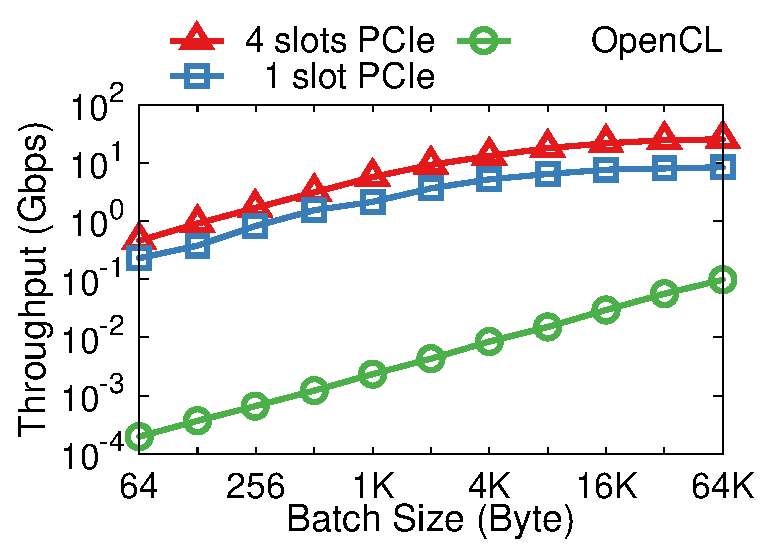
\includegraphics[width=0.5\textwidth]{eval/pcie_1}
	}
	\subfloat[]{
		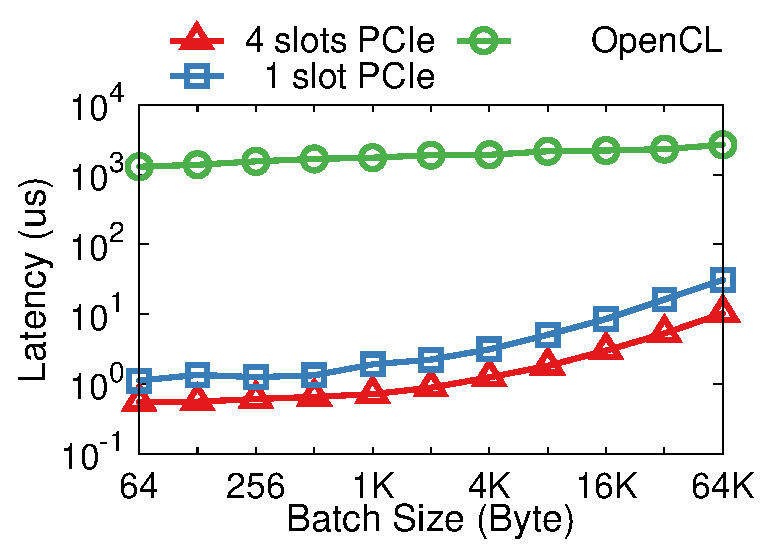
\includegraphics[width=0.5\textwidth]{eval/pcie_2}
	}

	\caption{PCIe I/O 通道的性能。Y 轴是对数坐标系。}

	\label{clicknp:fig:pcie}
\end{figure}


\subsection{Verilog 元件}

对于一些元件(如乘法器阵列和调度器),高层次综合工具难以生成高效的硬件逻辑。为了节约面积和降低延迟,这些元件需要用硬件描述语言来编写。在 \name 中,每个元件被编译成一个 OpenCL 核(kernel),它被高层次综合工具编译成一个 Verilog 模块,使用 Altera Avalon ST 或 Xilinx AXI 接口连接管道,使用 Altera Avalon MM 或 Xilinx AXI 接口连接全局内存。为了把开发者用硬件描述语言编写的 Verilog 元件集成到系统中,开发者需要编写一个接口相同的空元件作为占位符(或功能相同的高级语言元件用于 CPU 调试与测试),并用 \textbf{verilog} 关键字在 \name 配置文件中声明。编译工具链会将高层次综合工具为占位符元件生成的 Verilog 模块替换为开发者的实现。


\iffalse
\subsection{调试与测试}

\name 提供三种方法用于调试与测试。

\textbf{CPU 功能仿真。}
\name 元件使用类 C 的高级语言编写,因此一个元件可以编译成 CPU 上运行的一个线程,而管道就是线程之间的队列。开发者可以使用熟悉的调试工具来调试功能和单元测试。

\textbf{时钟精确的硬件逻辑仿真。}
元件之间的通信管道有死锁的可能,在 CPU 功能仿真时由于时序与硬件逻辑不一致,不一定能发现问题。为此,\name 可以集成硬件开发者熟悉的硬件逻辑仿真框架,如 ModelSim。为了便于软件开发者使用,\name 封装了 printf 等日志语句。

查看 \textbf{.state} 变量的值……

\textbf{实际 FPGA 运行。}
硬件逻辑仿真速度很慢,不能反映实际性能,且难以测试与 PCIe DMA、网络之间的交互。

日志高速发送:通过 PCIe I/O 通道传输到主机上。

SignalTap

断点如何实现……

\subsection{元件热迁移和高可用}

\textbf{虚拟机热迁移,计算节点对应的网卡状态;网络、存储节点热迁移(升级,扩容等),网卡状态;高可用性,故障恢复……}

\textbf{热升级:不丢包,的时候原来的 FPGA 不处理了,buffer 起来。把旧 FPGA 的状态迁移到新 FPGA,让交换机开始往新 FPGA 的 buffer 里灌,然后从旧 FPGA 的 buffer 里把数据倒出来在新的 FPGA 里处理,处理完后开始处理新 FPGA 自己的 buffer,迁移结束。}

\textbf{高可用:状态机复制的方法,两个 FPGA 收到相同的数据包序列,只要元件内部没有随机化或与时间相关的处理逻辑,就能保证两个 FPGA 收到的数据包序列相同。检测到备份节点故障,只需启动一个新的备份节点,然后执行热升级操作。检测到主节点故障,切换输出到备份节点(可能出现少量数据包丢失或重复,TCP 可以安全地处理这些情况)。}
\fi

\egg{

\egg{
Control signals can only be generated by the manager thread. 
When the manager thread sends a signal to a target element in FPGA, it will embed the ID of the element in the signal message, and 
passes the message to \textit{CmdHub} through slot 32.
\textit{CmdHub} will parse the message and forward the signal request to corresponding elements, again through FIFO buffers. 
}



\egg{
As aforementioned, OpenCL advocates batch processing model where communication between host program and a kernel in FPGA must go through shared DRAM, and the host program cannot control the kernel while it is running.
We could use a special kernel to proxy messages between host program and the kernel via DRAM, but it incurs \approx1ms latency.
DDR access is performed via PCIe link and raw PCIe latency is merely \approx1$\mu$s. As we improve kernel communication efficiency with channels in place of shared memory, we design a host-kernel communication mechanism with channel abstraction for low latency and high throughput.
We leverage I/O channel in Altera OpenCL and AXI stream in Vivado 高层次综合 to connect the Catapult shell to kernels and built a PCIe bypass switch to arbitrate accesses for on-board DRAM and kernel I/O channel.

A PCIe link is split into multiple logically independent \textit{slots} which can operate in parallel.
One slot is reserved for signals. Remaining slots are assigned to channels between host and FPGA elements, so each channel can transfer data in parallel without head-of-line blocking.
On CPU side, each host element is run on a separate core and receives input flits via PCIe by polling or interrupt.
On FPGA side, each element that communicates with host is connected to an inbound demultiplexer and an outbound multiplexer, where load-adaptive batching is performed to improve peak throughput while preserving low latency under light load.
}

\egg{
With polling model, the latency of the PCIe I/O channel  is $< 2 \mu s$ when message size is small, but the latency will reach to $32 \mu s$
for full batched messages.
The interrupt model, however, will increase the latency.
}

\egg{
, where each slot is assigned to one CPU core. Our PCIe channel has two bottlenecks: (1) PCIe Gen2 x8 interface has 32 Gbps bandwidth, (2) PCIe data width is 128b and the clock frequency of Catapult shell is 200 MHz, which limits PCIe throughput to 25.6 Gbps. PCIe I/O channel offers 1\approx2$\mu$s RTT which translates to 400\approx800K host-kernel transactions per second. Polling mode yields lower latency and higher throughput, while interrupt mode latency can be improved by utilizing more cores and PCIe slots. Four CPU cores are sufficient to saturate maximum throughput for both polling and interrupt mode under 64KB batch size. Effectiveness of batching will be further evaluated in traffic dumper application.
}

}

%%!TEX root=main.tex
\section{应用}
\label{clicknp:sec:application}

为了评估 \name 的灵活性,我们基于 \name 开发了五个常见的网络功能,可以在我们的测试床中运行。
表 \ref {clicknp:tab:applications} 总结了每个网络功能中包含的元件数量和总代码行数,包括所有元件规范和配置文件。
经验证实,\name 的模块化架构极大地改善了代码重用并简化了新网络功能的构建。
如表 \ref {clicknp:tab:elements} 所示,在许多应用程序中有很多机会重用一个元件,例如,本文(A1-5)中所有五个网络功能都使用了L4\_Parser。
每个网络功能可能需要1个左右的时间才能让一个程序员进行开发和调试。
联合CPU / FPGA处理的能力也将极大地帮助调试,因为可以将有问题的元件移动到CPU,以便轻松地打印日志来跟踪问题。

下文将详细讨论这些网络功能。

\textbf {A1. 数据包生成器(PktGen)和捕获(PktCap)。}
PktGen可以根据不同的配置文件生成各种流量模式。
它可以生成不同大小的流,并根据给定的分布安排它们在不同的时间开始。
生成的流可以进一步通过不同的流量整形器来控制流速及其突发性。
PktCap只是将收到的所有数据包重定向到 \textit {logger} 元件,这些元件通常位于主机中。
由于单个记录器无法充分利用PCIe I / O通道容量,因此PktCap在FPGA中具有接收端缩放(RSS)元件,以根据流5元组的散列将数据包分发到多个记录器。
由于PCIe通道的容量小于40G 网卡的容量,添加了一个\textit {提取器}(extractor)元件,它只提取数据包的重要字段(例如,如果有5个元组,DSCP和VLAN标记),并转发这些字段(总共16B) ,以及跨PCIe的记录器元件的时间戳(4B)。
PktCap就是一个展示联合CPU / FPGA处理重要性的例子。
与FPGA相比,CPU具有更多的内存用于缓冲,并且可以轻松访问其他存储,例如,文献 \cite{lee2015flosis} 中的HDD / SSD驱动器,因此在CPU上运行记录器更有意义。


\textbf {A2. OpenFlow 防火墙(OFW)。}
Openflow~\cite {mckeown2008openflow} 防火墙支持流的精确匹配和通配符匹配。
精确匹配表是使用Cuckoo Hashing \cite{cuckoo} 实现的,包含与流5元组匹配的128K条目。
模糊匹配匹配基于TCAM。
但是,具有512个104位条目的简单TCAM实现占用了FPGA的65%逻辑资源。
相反,本章使用基于BRAM的TCAM \cite {jiang2013scalable}。
基于BRAM的TCAM将搜索密钥分解为8位密钥,并使用它们来寻址查找表,这些表将内存换成逻辑区域。具有2K条目的BRAM TCAM需要14%逻辑和43%的BRAM。
此外,本文设计了 HashTCAM,以利用流表中的许多条目共享相同的位掩码这一事实。
HashTCAM将表空间划分为许多较小的哈希表,每个哈希表都与一个位掩码相关联。
在查找哈希表之前,任何传入的数据包都将首先执行“和”操作。
表中的每个条目也与优先级相关联。
仲裁器(multiplexer)选择具有最高优先级的匹配条目。
HashTCAM在功能和区域成本之间有更好的权衡。
具有16K流条目和16个不同位掩码的HashTCAM(类似于Broadcom Trident II~\cite {broadcomethernet})需要19%逻辑和22%BRAM。
管理器程序总是尝试根据其位掩码对规则进行分组,并将具有大多数规则的组放入HashTCAM。
然后将其余规则放入基于BRAM的TCAM中,这些规则不适合HashTCAM中的任何组。


\textbf{A3. IPSec网关(IPSecGW)。}
软件网络功能的一个问题是,当数据包需要一些计算密集型处理时,CPU很快就会成为瓶颈,例如,IPSec \cite {packetshader}。
IPSec数据面需要使用AES-256-CTR加密和SHA-1身份验证处理IPSec数据包。
如 \S \ref {clicknp:subsec:lib} 所示,单个AES\_CTR元件只能实现27.8~Gbps的吞吐量。因此,需要两个AES\_CTR元件并行运行以实现线速率。
然而,SHA-1很棘手。 SHA-1将数据包分成较小的数据块(64B)。
虽然一个数据块中的计算可以流水线化,但是一个IP数据包内的连续块之间存在依赖关系 - 下一个块的计算无法在前一个块完成之前开始!
如果按顺序处理这些数据块,吞吐量将低至1.07 Gbps。
幸运的是,可以利用不同数据包之间的并行性。
虽然当前数据包的数据块的处理仍在进行,但提供了不同数据包的数据块。
由于这两个数据块没有依赖关系,因此可以并行处理它们。
为了实现这一点,我们设计了一个名为 \textit {reservo} 的新元件(保留站的简称),它可以缓冲多达64个数据包,并为SHA-1元件调度独立的块。在计算了一个数据包的签名之后,\textit {reservo} 元件将它发送到将SHA-1 HMAC附加到数据包的下一个元件。
还有一件棘手的事情。
虽然SHA-1元件具有固定的延迟,但数据包的总延迟是不同的,即与数据包大小成比例。
当在SHA-1计算中调度多个分组时,这些分组可能是无序的,例如,大分组后面的较小分组可能更早地完成。
为了防止这种情况,在SHA-1元件之后进一步添加了一个\textit {reorder buffer}元件,该元件存储无序数据包并根据数据包的序列号恢复原始顺序。

\textbf {A4. L4负载平衡器(L4LB)。}
L4 负载平衡器根据Ananta~ \cite {ananta}中的\textit {multiplexer}(MUX)实现。
MUX服务器基本上查看数据包标头,并查看是否已为该流分配了\textit {直接地址}(DIP)。
如果是,则通过NVGRE隧道将分组转发到由DIP指示的服务器。否则,MUX服务器将调用本地控制器为流分配DIP。
MUX服务器中需要按流状态。
由于存在故障并且避免黑洞需要即时更改后端服务器列表,因此无法使用基于散列的ECMP。此外,高级LB还可能需要负载感知平衡。
流表用于记录流向其DIP的映射。
为了处理数据中心的大流量,它需要L4LB在流表中支持多达3200万个流。
显然,如此大的流量表不能适应FPGA的BRAM,必须存储在板载DDR存储器中。
但是,访问DDR内存很慢。
为了提高性能,在BRAM中创建了一个带有16K高速缓存行的4路关联流缓存。最近最少使用(LRU)算法用于替换流缓存中的条目。

在本章的实现中,传入的数据包首先传递一个\textit {解析器}(parser)元件,该元件提取5元组并将它们发送到\textit {流缓存}(flow cache)元件。
如果在流缓存中找不到流,则将数据包的元数据转发到全局流表,该表读取DDR中的完整表。
如果仍然没有匹配的条目,则该数据包是流的第一个数据包,并且请求被发送到\textit {DIPAlloc}元件,以根据负载平衡策略为该流分配DIP。
确定DIP后,将一个条目插入到流表中。

在确定分组的DIP之后,封装元件将检索下一跳信息,例如IP地址和VNET ID,并相应地生成NVGRE封装的分组。
对于流的剩余分组,从流状态提取DIP。
如果收到FIN数据包或发生超时,则流条目将无效
在从流中接收任何新数据包之前。
在确定DIP之后,从BRAM检索下一跳元数据并封装NVGRE头以将分组引导到分配的DIP。

除了\textit {DIPAlloc}元件之外,所有元件都放在FPGA中。
由于只有流的第一个数据包可能会出现\textit {DIPAlloc}并且分配策略也可能很复杂,因此更适合运行
CPU上的\textit {DIPAlloc},是联合CPU-FPGA处理的另一个例子。

%
\egg{
To handle the large traffic volume in datacenters, it requires the L4LB to support up to 32 million flows in the flow table.
Clearly, such a large flow table cannot fit into the BRAM of FPGA, and has to be stored in onboard DDR memory.
Accessing DDR memory is slow. To improve performance, we further create a 4-way associative flow cache in BRAM with 16K 
cache lines. The flow cache is replaced based on the Least Recently Used (LRU) algorithm.
DDR memory access is a fat pipeline stage as shown in Figure \ref{clicknp:fig:unbalance}. We move the DDR access part to a separate element to make the fast path run asynchronously with slow path.}



\textbf {A5. pFabric 流调度程序。}
最后,使用\name 来实现一个最近提出的数据包调度规则--pFabric \cite {pfabric}。
pFabric调度很简单。它只保留浅缓冲区(32个数据包),并始终使具有最高优先级的数据包出列。当缓冲区已满时,优先级最低的数据包将被丢弃。
pFabric显示在数据中心中实现接近最佳的流完成时间。
在原始论文中,作者提出使用二进制比较树(Binary Comparison Tree,BCT)来选择具有最高优先级的数据包。
但是,虽然BCT只需要$O(log_2 N)$个周期来计算最高优先级的数据包,但在连续的选择过程之间存在依赖关系。这是因为只有当前一个选择完成后才能知道最高优先级的数据包,然后才能可靠地启动下一个选择过程。
这种限制要求时钟频率至少为300MHz才能实现40Gbps的线速,这对当前的FPGA平台来说是不可能的。
本文使用不同的方式来实现pFabric调度程序,它更容易并行化。
该方案基于\textit{移位寄存器优先级队列}(shift register priority queue) \cite {moon2000scalable}。
条目以非增加优先级顺序保存在$K$个寄存器中。
出列时,所有条目都向右移动并弹出头部。这只需要1个周期。
对于入队操作,新数据包的元数据将转发到所有条目。
现在,对于每个条目,可以在条目中的分组,新分组和相邻条目中的分组之间执行本地比较。
由于所有局部比较都可以并行进行,因此入队操作也可以在1个周期内完成。
入队和出队操作可以进一步并行化。
因此,可以在一个周期中处理分组。

\iffalse
\textbf{A6. 容错的 LTE SPGW。}

\textbf{A7. 端口扫描检测。}

\textbf{A8. HTTPS RSA 加速。}

\textbf{A9. 正则表达式匹配。}

\textbf{A10. 神经网络推理。}
\fi

\egg{
pFabric \cite{alizadeh2013pfabric} is a near-optimal datacenter transport based on priority scheduling and dropping. Packets are scheduled based on its flow size or remaining flow size in a small queue. Our pFabric scheduler implementation (Figure \ref{clicknp:fig:PFabric}) support 4-giga strict priorities, including a PriorityQueue which deques the packet with highest priority and drops overflow packets with lowest priority, a ReorderQueue to find the earliest packet from the flow with highest priority to avoid starvation and keep packet ordering, and a PacketBuffer to receive packets into buffer and schedule or drop packets out of buffer. Since queue size in a perfectly load balanced fabric should be small, we choose shift register priority queue for maximum throughput and clock frequency.

ReorderQueue is another shift register queue ordered by flow hash. On enque command from PacketBuffer, packet metadata with flow hash $f_{new}$ is enqued to entry $i$ where $f_{i-1} < f_{new} \leq f_{i}$. On deque command from PriorityQueue, the entry $i$ with $f_{i} = f_{deque} < f_{i+1}$ is dequed. Packets with a same flow hash are dequed in the same order as they are enqued.


\begin{figure}[h!]
	\centering
	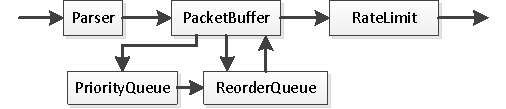
\includegraphics[width=1.0\columnwidth]{image/PFabric}
	\vspace{-0.30in}
	\caption{PFabric Element Graph}
	\vspace{-0.10in}
	\label{clicknp:fig:PFabric}
	%    
\end{figure}
}

%\section{ClickNP Language}
\label{clicknp:sec:language}

\subsection{Element Graph}

The ClickNP script defines a directed graph of elements and channels, which adapts some syntax from the Click modular router \cite{kohler2000click}.

The following ClickNP script and figure \ref{clicknp:fig:ClickNPScriptExample} define the network card-to-ToR part of a network application with NVGRE encapsulation and Per-VM rate limiting.

\begin{figure}[!t]
	\centering
	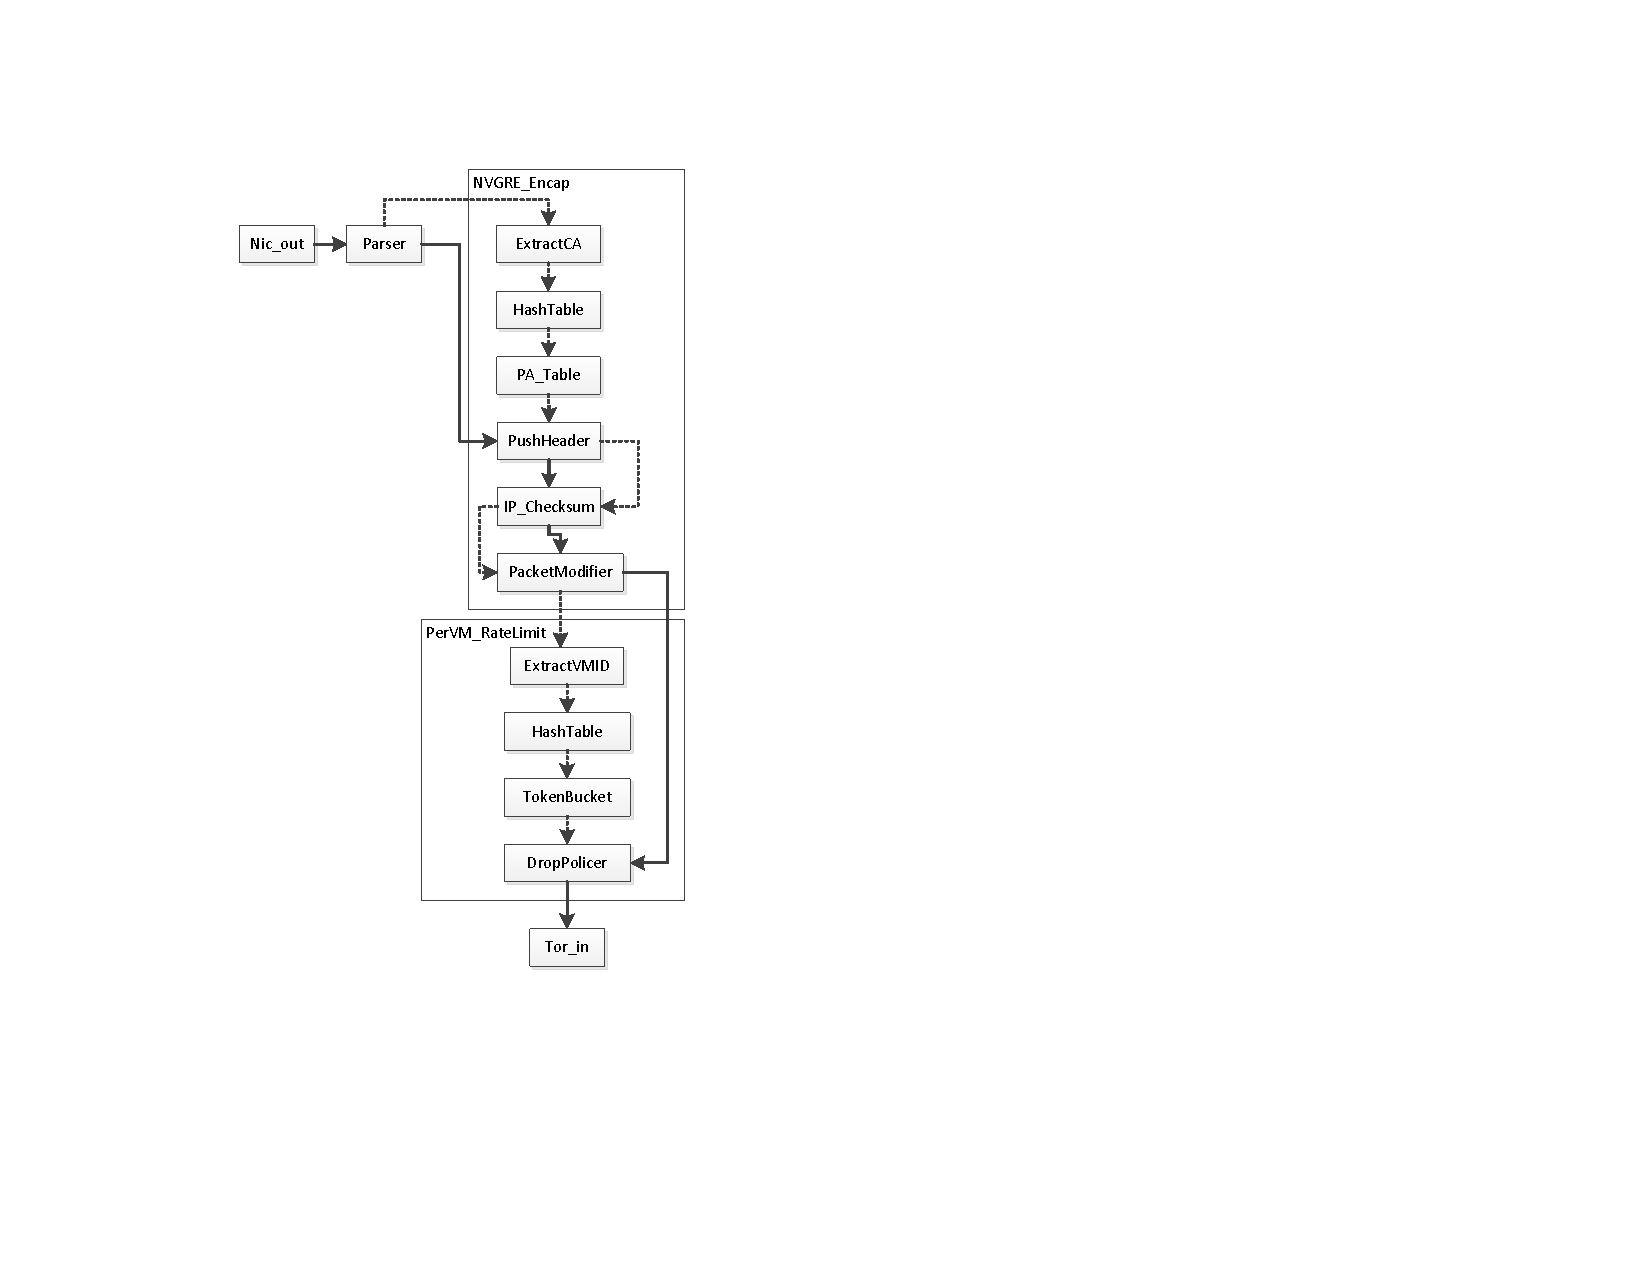
\includegraphics[width=1.0\columnwidth]{image/ApplicationExample}
	\vspace{-0.25in}
	\caption{NVGRE Encap + Rate Limiting in ClickNP}
	\vspace{-0.15in}
	\label{clicknp:fig:ClickNPScriptExample}
	%    
\end{figure}

\begin{lstlisting}
.element_group NVGRE_Encap {
    PushHeader :: encap (2,2)
    begin[1] -> [1]encap -> IP_Checksum (2,2) -> PacketModifer (2,2) -> end
    begin[2] -> ExtractCA (1,1) -> HashTable @ (1,1,14) -> PA_Table @ (1,1) -> [2]encap
}
.element_group PerVM_RateLimit {
    DropPolicer :: action (2,2)
    begin[1] -> [1]action -> end
    begin[2] -> ExtractVMID (1,1) -> HashTable @ (1,1,4) -> TokenBucket @ (1,1) -> [1]action
}
PerVM_RateLimit :: ratelimit (2,2)
nic_out -> Parser (1,2) -> NVGRE_Encap (2,2) -> ratelimit[1] -> tor_in
ratelimit[2] -> Drop (1,0)
\end{lstlisting}

Per clock cycle, each element can read at most one 64-byte message from each input channel and write zero or one 64-byte message to each output channel. A channel either passes \textit{flit} messages (solid line) or \textit{metadata} messages (dotted line). Each flit contains 32 bytes of packet content and flags indicating the start of a packet (sop) and the end of a packet (eop). The metadata format is user-defined, containing the parsed packet header and optionally a subsequent action.

Lines 1--5 define an \textit{element group} of 6 elements. Line 2 instantiates a \textit{PushHeader} element with the name \textit{encap}. Numbers in parentheses stand for the number of input and output ports, and optional subsequent numbers are element parameters (see section \ref{clicknp:subsec:elementdef}). Square brackets indicate the port number to be connected via channel. The ``@'' symbol indicates on-the-fly host control.

The metadata, which includes parsed packet headers, is directed into the element group via port 1. Here, the Customer Address (CA) is extracted and compared with a \textit{HashTable} that is controlled by the host program. The result of this comparison is then used as an index for the Physical Address (PA) table (also controlled by the host program). The PA table modifies the action part of the metadata to include the outer header offset, length, and data. The metadata, along with packet content flits stored in the channel, is sent to the \textit{PushHeader} element where the packets are actually shifted. The metadata (with the action cleared) and packet flits then proceed to the \textit{IP\_Checksum} element where a new IP header checksum is calculated and a packet modify action is generated to update the IP checksum field in the subsequent \textit{PacketModifier} element.

Our decision to separate flit and metadata messages was made not only for clarity but also for performance. One reason is to reduce the throughput load of lookup tables. Typically, table lookup is performed once per packet, while each Ethernet packet contains 2--48 flits. If flits are passed through via lookup tables, we can process at most one flit per cycle. To achieve line rate, we need to complete each iteration in one cycle, but lookup tables that both read and write to local memory require two cycles due to memory timing.

Another reason for separating flit and metadata is to pipeline packet modification actions. For instance, in the \textit{IP\_Checksum} action, the IP header spans the boundary of the first and second flits. Therefore, the checksum can only be calculated after the first two flits have arrived. However, the IP checksum field that needs to be updated is in the first flit. If we use one channel for both flit and metadata, then the element has to output nothing in the first cycle processing a packet. As discussed in section \ref{clicknp:subsec:designgoals}, such per-packet idle cycle is unacceptable for our line-rate FPGA implementation. By transferring flit and metadata in separate channels, the \textit{IP\_Checksum} element can pass through flits while calculating the checksum, and flits are buffered in the channel between the \textit{IP\_Checksum} and \textit{PacketModifier} elements. When the \textit{PacketModifier} receives the metadata containing the IP checksum, the first flit is also ready. This coding style eliminates the need for buffers within elements, which consume more resources than buffers within channels.

A network application is typically constructed with a parser and a sequence of network functions. A network function initially creates a lookup key from the parsed packet header, matches the key in a lookup table (section \ref{clicknp:subsec:lookuptables}), and then constructs an action based on the match result. The action and packet flits are subsequently passed into an action element. This coding convention allows lookup table elements to be generic, actions to be chained, network functions to be chained, and packet parser to be shared.

\subsection{Element Definition}
\label{clicknp:subsec:elementdef}

An element comprises five components: states, ports, an initializer, a data handler, and a signal handler.

\textit{States} delineate variables that persist throughout the element's lifecycle. Each element has several input and output \textit{ports}, the number of which is configured by the element graph. The \textit{Initializer} is executed once immediately after the element is launched. The main processing loop consists of a data handler (\textit{.handler}) and a signal handler (\textit{.signal}).

Each element instance with host control enabled (denoted by the "@" symbol) is connected to two special kernels, \textit{CmdHub\_in} and \textit{CmdHub\_out}. \textit{CmdHub\_in} is a demultiplexer from PCIe input to signal-enabled kernels, while \textit{CmdHub\_out} is a multiplexer from signal-enabled kernels to PCIe output. For each iteration, if there is a signal input from the host program, the signal is unmarshaled from the PCIe packet to an \textit{event}, the signal handler is invoked, then the \textit{outevent} is marshaled to a PCIe packet and sent back to the host. Otherwise, input channels are checked for a new message, the data handler is invoked, and then output channels are written.

The data handler should verify whether its input ports have a message ready, read states, perform calculations, write back changes to states, optionally write to output ports, and return which input ports are to read in the next iteration. Each input port has a buffer of one message size, and a handler is free to consume or not consume the message by calling or not calling \textit{clear\_input\_ready}. If there are multiple calls to \textit{set\_output\_port} for the same port in one iteration, only the last call will be effective.

The \textit{IP\_Lookup} element below is a binary-tree based IP classifier. The number of nodes per tree level is controlled by the third parameter in element instantiation. The element reads IP address from input port 1, consults the table and writes result to output port 1.

To reduce resource utilization in FPGA, the host program should keep an exact copy of the tree structure, and the assignment of nodes for rule update is handled by host program. The signal handler executes node update instructions from host program. The read interface in signal handler is for crash recovery of host program, so that the restarted host program can rebuild the tree from FPGA.

\begin{lstlisting}
.element IP_Lookup {
    .state {
        // levels of binary tree
        constexpr DEPTH = 32;
        // max entry num per level
        constexpr WIDTH = $3;
        .repeat (depth, 0, DEPTH) {
            constexpr w = ((1<<depth) < WIDTH ? (1<<depth) : WIDTH);
            short value$depth[w];
            short left$depth[w];
            short right$depth[w];
        }
    }
    .init { }
    .handler {
        if ( !input_ready(PORT_1) )
            return PORT_1;
        bool *ip = (bool *) &input_data[1];
        clear_input_ready(PORT_1);

        short pos = 0;
        short result = 0;
        .repeat (depth, 0, DEPTH) {
            result = value$depth[pos];
            if (ip[depth])
                pos = left$depth[pos];
            else
                pos = right$depth[pos];
            if (pos == 0)
                BREAK;
        }
        set_port_output(1, result);
        return PORT_1;
    }
    .signal (uchar cmd, uchar depth, uint pos, uint value, uint left, uint right) {
        uint pos = event.pos;
        .repeat (i, 0, DEPTH) {
          if (i == event.depth)
            switch (event.cmd) {
              case 1: // update
              value$i[pos] = event.value;
              left$i[pos]  = event.left;
              right$i[pos] = event.right;
              break;
              case 2: // read
              outevent.value = value$i[pos];
              outevent.left  = left$i[pos];
              outevent.right = right$i[pos];
              break;
            }
        }
    }
}
\end{lstlisting}

The command \textit{.repeat (depth, 0, DEPTH)} generates \textit{DEPTH} copies of code with the string \textit{\$depth} replaced with 0, 1, 2... up to \textit{DEPTH}-1. \textit{BREAK} is a special statement used to jump to the end of repeated code blocks. The following illustrates the storage regions for variables.

\begin{itemize}
	\item State arrays \textit{value}n, \textit{left}n, and \textit{right}n are compiled to (3 * \textit{DEPTH}) SRAM blocks. Each array is read (in handler) or written (in signal) once per iteration, allowing the element to be fully pipelined.
	\item Local variables \textit{ip}, \textit{pos}, and \textit{result} are intermediate variables in the combinational logic and will not occupy any storage space on the FPGA.
	\item Loop control variables \textit{depth} and \textit{i}, as well as \textit{constexpr}s, are syntactic sugar for code generation.
\end{itemize}

The tree lookup logic in lines 23--31 is automatically pipelined by the ClickNP toolchain. After data flow analysis, variables \textit{pos} and \textit{result} are each split into multiple variables in single static assignment (SSA) form. Since SRAM read has a one-cycle latency, the lookup will take at least \textit{DEPTH} cycles. Fortunately, these memory read operations can be pipelined. A pipeline with \textit{DEPTH} stages is inferred, each stage holding a copy of live variables \textit{ip}, \textit{pos}, and \textit{result} in registers. Different stages of the pipeline process different copies of live variables (i.e., different copies of input data) simultaneously. Pipelining improves throughput by exploiting temporal parallelism.

The tree update logic in lines 41--43 are independent, so the three memory writes are performed in parallel, which improves throughput by exploiting spatial parallelism.

\subsection{Host Communications}

The signal handler is a stop-and-wait mechanism for host-to-kernel communication. Kernels also need to initiate communications, for example, to send alerts, dump packets, and use host memory as a cache. We develop a streaming interface for kernels to communicate with the host program via channels as if the host program was another kernel. To use the streaming host interface, an element connects to the \textit{host\_in} pseudo-element for input and \textit{host\_out} for output.

The ClickNP compiler generates a C++ class for each element type, including 5 methods:
\begin{itemize}
	\item \textit{launch}, which launches the corresponding kernel.
	\item \textit{signal}, which marshals parameters, sends an event to the signal handler, waits to receive an outevent, and unmarshals the response.
	\item \textit{send}, which sends a message to the kernel via the streaming interface.
	\item \textit{receive}, which receives a message (block or non-block) from the kernel via the streaming interface.
	\item \textit{setCallback}, which, if set, calls the callback function every time a message is received via the streaming interface.
\end{itemize}

The C++ class can be extended to add more methods with clearer semantics. For example, the \textit{IP\_Lookup} class provides methods \textit{addRule}, \textit{deleteRule}, \textit{clearTable}, and \textit{reloadTable} to encapsulate the internal states of the IP lookup tree and a series of node update operations needed for one rule update.

All element classes share a common base class, \textit{Element}, and the ClickNP compiler generates a \textit{std::map} of element names and element class instances. A host program should first initialize the platform, then execute the \textit{launch} method of each element object.

%%!TEX root=main.tex
\section{ClickNP Elements}
\label{clicknp:sec:elements}

In this section we show LOC (Line Of Code) (excluding host program) and resource utilization of some common elements under reasonable parameter settings.

All elements shown in this section can process 40 Gbps line rate for all Ethernet packet sizes under 190 MHz clock rate, i.e. one cycle per iteration for elements processing packet flits, and up to 3 cycles per iteration for elements processing metadata only.

\subsection{Basic Connectors}

\begin{table}[h!]
	\centering
	\label{clicknp:tab:Basic Connectors}
	\begin{tabular}{l|r|r|r}
		Element & LOC & Logic & Memory \\
		\hline
		Tee	&  & \%  & 0\% \\
		Mux	&  & \% & 0\% \\
		Demux & & \% & 0\% \\
		FlitMux & & \% & 0\% \\
		FlitDemux & & \% & 0\% \\
	\end{tabular}
\end{table}


\subsection{Programmable Header Parser}

Packet parser is an important part of network processor, whose complexity comes from tunneling protocols and diversity of protocols in each layer.

The uncertainty of outer layers introduce non-constant header offset in the packet. For example, an Ethernet packet without VLAN has IP header offset 14, an Ethernet packet with VLAN has IP header offset 18. Simply using a variable as index to packet byte array is very ineffective in OpenCL. An array with one or more variable index access will be implemented as block SRAM in FPGA, which only support one read operation per cycle. In order to parse the packet header (which includes many array accesses) in one cycle, we need to implement the packet buffer as register in FPGA, which requires all accesses to the packet buffer array to have constant index.

%If we create an element for each packet header, then each element needs to shift the packet payload in order to ``peel off'' the parsed header. The first drawback is that each element introduces some overhead in logic utilization. Since there are multiple leaf elements representing the innermost header to parse, and different elements have different latencies, output packets at the final mux will be out-of-order. The reordering buffer would take considerable local memory. Furthermore, in the case of network virtualization and tunneled protocols, there will be a loop of elements that each tunneled packet would travel twice, which lowers throughput of packet parser.

To implement a packet parser with all packet buffer offsets to be constant, without shifting packet payload after each header is parsed, we need to enumerate all possible parsing paths (e.g. Ethernet $\rightarrow$ IP, Ethernet $\rightarrow$ VLAN $\rightarrow$ IP), duplicate parser code for each path and calculate offset for each access to packet buffer. Doing such work manually is frustrating and error-prone, therefore ClickNP provides a general \textit{.state\_machine} abstraction, which can generate a decision tree composed of all possible state migration paths and calculate all packet buffer offsets at compilation time.

\begin{lstlisting}
.state_machine {
    constexpr offset = 0;
    .parser_define MAX_STATE_REPEAT 2;
    begin {
        constexpr offset += 12;
        ushort next_proto = *(ushort *) &input[offset];
        constexpr offset += 2;
        if (next_proto == PROTO_VLAN)
            .goto_state VLAN;
        else if (next_proto == PROTO_IPv4)
            .goto_state IPv4;
        else
            .goto_state end;
    }
    VLAN {
        if (!meta.vlan)
            meta.vlan = *(ushort *) input[offset];
        ushort next_proto = *(ushort *) &input[offset + 2];
        constexpr offset += 4;
        if (next_proto == 0x8100)
            .goto_state VLAN;
        else if (next_proto == 0x0800)
            .goto_state IPv4;
        else
            .goto_state end;
    }
    IPv4 {
        .if (STATE_REPEAT == 1) {
            meta.src_ip = *(uint *) &input[offset + 12];
            meta.dst_ip = *(uint *) &input[offset + 16];
        } .else {
            meta.inner_src_ip = *(uint *) &input[offset + 12];
            meta.inner_dst_ip = *(uint *) &input[offset + 16];
        }
        ushort next_proto = input[offset + 9];
        constexpr offset += 20;
        if (next_proto == 94)
            .goto_state IPv4; // IP-in-IP
        else if (next_proto == 97)
            .goto_state begin; // ETHERIP
        else
            .goto_state end;
    }
}
\end{lstlisting}


\begin{figure}[!t]
	\centering
	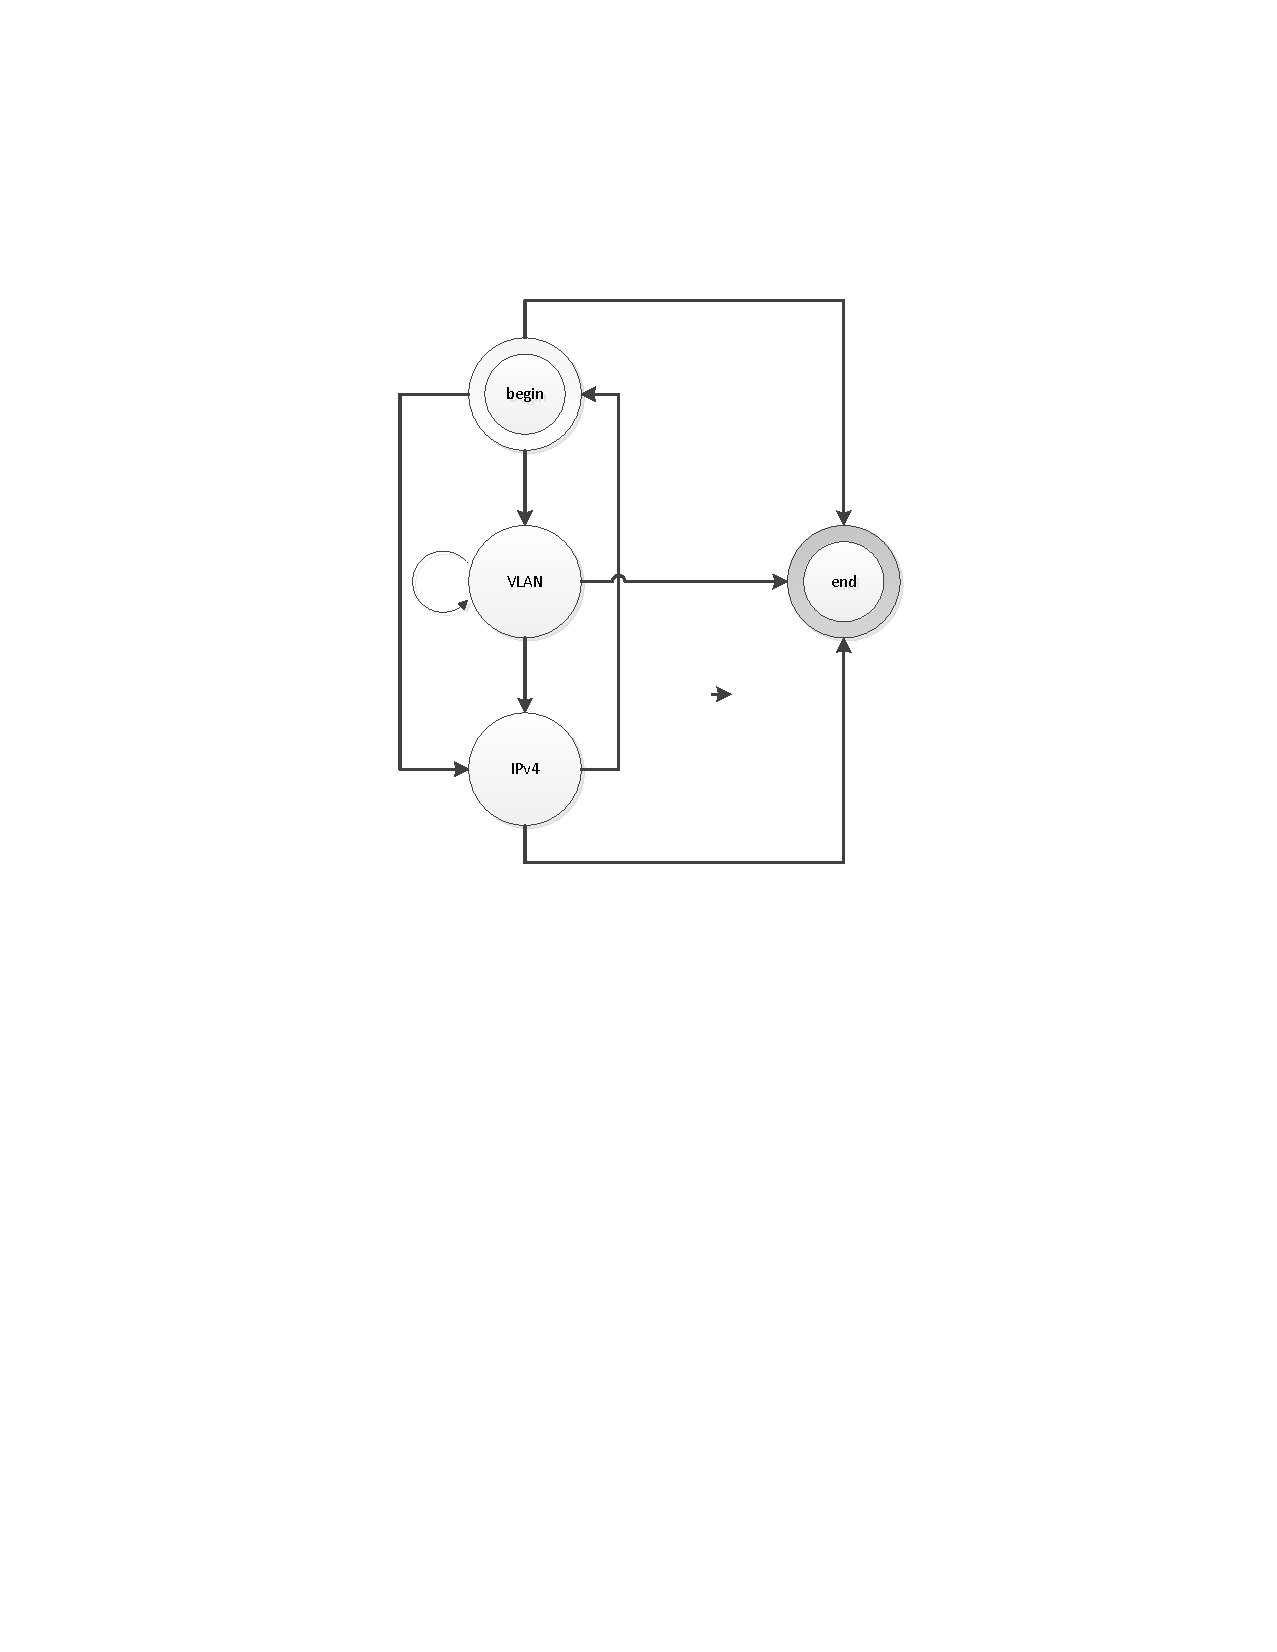
\includegraphics[width=0.7\columnwidth]{image/StateMachine}
	\vspace{-0.15in}
	\caption{Sample State Machine for Header Parser}
	\vspace{-0.15in}
	\label{clicknp:fig:StateMachine}
	%    
\end{figure}

Above code implement a sample header parser in figure \ref{clicknp:fig:StateMachine}, each state is set to repeat at most twice. 44 lines of code with 3 states generates 314 lines of code with 27 states, which takes 2\% logic resource.

Following show some parsers to extract metadata from some well-known protocols. The element code can be easily modified to extract new fields or incorporate new protocols.

\begin{table}[h!]
	\centering
	\label{clicknp:tab:PacketParsers}
	\begin{tabular}{l|r|r|r}
		Element & LOC & Logic & Memory \\
		\hline
		EthVlanParser & & \% & \% \\
		IPv4\_Parser & & \% & \% \\
		IPv6\_Parser & & \% & \% \\
		FlowTuple\_Parser & & \% & \% \\
		TCP\_Parser & & \% & \% \\
		NVGRE\_Parser & & \% & \% \\
		VXLAN\_Parser & & \% & \% \\
	\end{tabular}
\end{table}

\subsection{Lookup Tables}
\label{clicknp:subsec:lookuptables}

\textit{HashTable} is implemented using Cuckoo hash \cite{pagh2004cuckoo} with two memory banks, which can be used for exact matching.

\begin{figure}[h!]
	\centering
	
\includegraphics[width=0.6\columnwidth]{image/logo}
	\vspace{-0.15in}
	\caption{HashTable Collision Rate, x: occupancy, y: hash collision rate, lines: sequential IP, sequential port, random, theory}
	\vspace{-0.15in}
	\label{clicknp:fig:HashTableCollisionRate}
	%    
\end{figure}

\textit{TCAM} compares all entries in parallel and finds the lowest entry index that matches. Due to high logic resource utilization of TCAMs, we design \textit{HashTCAM} to trade off logic with memory. The design bases on an observation that bit-mask patterns in a set of real-world wildcard rules are limited. In order to reduce bit width of match key, commodity switching chips require users to specify bit-mask patterns prior to rule insertion, e.g. Broadcom Trident II \cite{broadcomethernet} only supports 16 bit-mask patterns.

HashTCAM also imposes a limitation on number of bit-mask patterns. For each unique bit-mask pattern, HashTCAM allocates a HashTable and fills its mask field. All rules sharing this bit-mask pattern can be inserted into HashTable whose key is masked original key and value is the index in original TCAM. Match results from HashTables are arbitrated to find the lowest index (highest priority) and get match result by index from SRAM. The \textit{HashTCAM} class in host program provides TCAM-like interface to abstract away HashTable allocation, rule update and SRAM update.

\begin{figure}[h!]
	\centering
	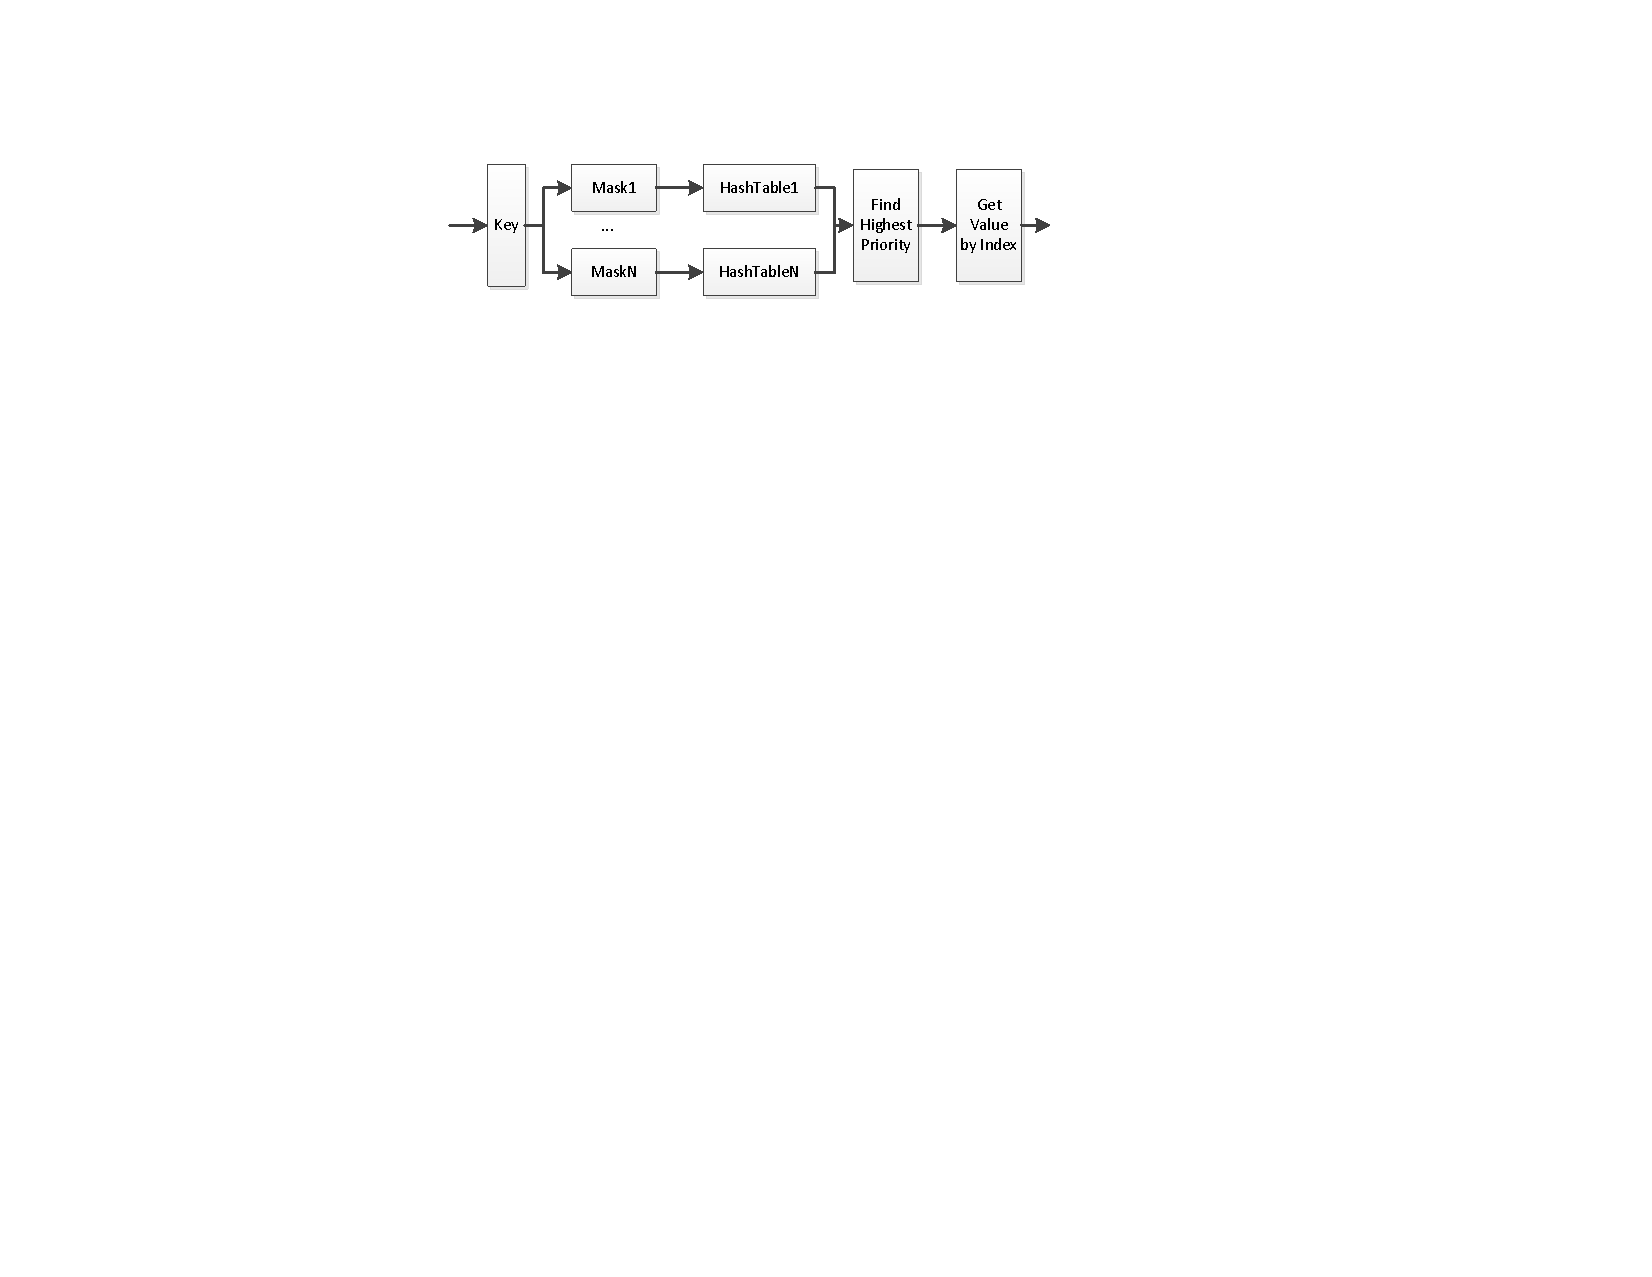
\includegraphics[width=1.0\columnwidth]{image/HashTCAM}
	\vspace{-0.30in}
	\caption{HashTCAM Architecture}
	\vspace{-0.10in}
	\label{clicknp:fig:HashTCAM}
	%    
\end{figure}

Longest Prefix Match (\textit{LPM}) is essentially the \textit{IP\_Lookup} example in section \ref{clicknp:subsec:elementdef}.

HashTable, TCAM, HashTCAM and LPM tables all match metadata, while deep packet inspection requires matching packet content. Content matching is much more resource hungry than matching a fixed offset in packet. \textit{StringMatch} works by comparing all offsets of a flit with the pattern byte-by-byte in parallel. \textit{RegexMatch} compiles multiple regexes into one 网络功能A (nondeterministic finite automaton) and build a 32-level pipeline to process next byte and update 网络功能A's active states every stage, similar to the \textit{IP\_Lookup} example. Due to logic resource constraint, current implementation of \textit{RegexMatch} compiles the 网络功能A into FPGA image and does not allow on-the-fly regex reconfiguration.

\begin{table}[h!]
	\centering
	\label{clicknp:tab:LookupTables}
	\begin{tabular}{l|r|r|r|r|r}
		Element & LOC & Key width & Size & Logic & Memory \\
		\hline
		HashTable 	& & 104b & 32K 	& 5\%  & 10\% \\
		TCAM 		& & 104b & 64	& 20\% & 0\% \\
		HashTCAM 	& & 104b & 16K    & 10\% & 10\% \\
		LPM			& & 32b  & 16K    & 10\% & 10\% \\
		StringMatch & & 32B  & 100	& & \\
		RegexMatch  & & 32B  & 100  & & \\
	\end{tabular}
\end{table}

Most signal handlers take only several cycles, so the update rate for lookup tables is bounded by the latency of PCIe channel: 120K updates per second in interrupt mode and 500K updates per second in polling mode.

\subsection{Packet Modifications}

\begin{table}[h!]
	\centering
	\label{clicknp:tab:PacketModElements}
	\begin{tabular}{l|r|r|r}
		Element & LOC & Logic & Memory \\
		\hline
		PacketModifier 	& & \% & 0\% \\
		PushHeader		& & \% & 0\% \\
		PopHeader		& & \% & 0\% \\
		DropPolicer 	& & \% & \% \\
	\end{tabular}
\end{table}

\subsection{Traffic Schedulers}

\begin{table}[h!]
	\centering
	\label{clicknp:tab:TrafficSchedulers}
	\begin{tabular}{l|r|r|r}
		Element & LOC & Logic & Memory \\
		\hline
		GenericPriorityQueue 	& & \% & 0\% \\
		RoundRobin		& & \% & 0\% \\
		WeightRoundRobin		& & \% & 0\% \\
		StrictPriority		& & \% & 0\% \\
		TokenBucket 	& & \% & \% \\
	\end{tabular}
\end{table}

%!TEX root=main.tex
\section{应用}
\label{clicknp:sec:application}
\label{clicknp:sec:eval}

\subsection{测试床与方法}

为了评估 \name 的灵活性,我们基于 \name 开发了五个常见的网络功能,可以在我们的测试床中运行。
表 \ref {clicknp:tab:applications} 总结了每个网络功能中包含的元件数量和总代码行数,包括所有元件规范和配置文件。
经验证实,\name 的模块化架构极大地改善了代码重用并简化了新网络功能的构建。
如表 \ref {clicknp:tab:elements} 所示,在许多应用程序中有很多机会重用一个元件,例如,本文(A1-5)中所有五个网络功能都使用了L4\_Parser。
每个网络功能可能需要1个左右的时间才能让一个程序员进行开发和调试。
联合CPU / FPGA处理的能力也将极大地帮助调试,因为可以将有问题的元件移动到CPU,以便轻松地打印日志来跟踪问题。

本章在16台Dell R720服务器的测试台中评估\name。
对于每个FPGA板,两个以太网端口都连接到架顶式(ToR)Dell S6000交换机\cite {dells6000}。
所有\name 网络功能都在Windows Server 2012 R2上运行。
本章比较\name 与其他最先进的软件网络功能。
对于在Linux上运行的那些网络功能,使用内核版本为3.10的CentOS 7.2。
测试使用PktGen发包工具以不同的速率生成具有不同数据包大小的测试流量(64B 数据包,最高吞吐量为 56.4 Mpps)。
为了测量网络功能处理延迟,在每个测试数据包中嵌入了一个生成时间戳。
当数据包通过网络功能时,它们被循环回到PktCap抓包工具,该PktCap与PktGen位于同一FPGA中。
然后可以通过从数据包的接收时间中减去生成时间戳来确定延迟。
由PktGen和PktCap引起的延迟通过直接环回(无网络功能)进行预校准,并从数据中删除。

\egg{
To measure 网络功能 processing latency, we forward packets to an \textit{Echo} server using the second port. 
The Echo server runs an \textit{Echo} function in its FPGA, which simply bounces all packets back to the source. 
%
Then, we can compare the difference between the timestamps of a packet 
when it first arrives and when the processed packet is bounced back, to obtain the latency 
with nanosecond accuracy.
%
The delay induced by the Echo server was pre-calibrated and removed from our data.
In our test, we use PktGen to generate testing traffic, which can 
generate packets at up to 56.4 Mpps (64B packets).
}

\egg{
Ethernet ports of FPGAs and servers are connected to a Dell S6000 40GbE switch 
FPGAs are installed on Windows Server 2012 R2.
CPU-based benchmarks are performed on 

We use TrafficGen application to benchmark throughput and latency.
TrafficGen application generates a given traffic pattern or replays a trace, embeds timestamp in packet payload and sends to tor\_out.
Applications forward packets from tor\_in to nic\_out. When TrafficGen receives packet from nic\_in, the timestamp is extracted from payload to measure latency.
The wire loopback RTT of TrafficGen is 0.85$\mu$s for 64B packets and 1.39$\mu$s for 1504B packets, which is the system error in all latency numbers we present.
}

\subsection{数据包生成器和抓包工具}
数据包生成器(PktGen)可以根据不同的配置文件生成各种流量模式。
它可以生成不同大小的流,并根据给定的分布安排它们在不同的时间开始。
生成的流可以进一步通过不同的流量整形器来控制流速及其突发性。
抓包工具(PktCap)将收到的所有数据包重定向到 \textit {logger} 元件,这些元件通常位于主机中。
由于单个记录器无法充分利用PCIe I / O通道容量,因此PktCap在FPGA中具有接收端缩放(RSS)元件,以根据流5元组的散列将数据包分发到多个记录器。
由于PCIe通道的容量小于40G 网卡的容量,添加了一个\textit {提取器}(extractor)元件,它只提取数据包的重要字段(例如,如果有5个元组,DSCP和VLAN标记),并转发这些字段(总共16B) ,以及跨PCIe的记录器元件的时间戳(4B)。
PktCap就是一个展示联合CPU / FPGA处理重要性的例子。
与FPGA相比,CPU具有更多的内存用于缓冲,并且可以轻松访问其他存储,例如,文献 \cite{lee2015flosis} 中的HDD / SSD驱动器,因此在CPU上运行记录器更有意义。


\subsection{OpenFlow 防火墙}
Openflow~\cite {mckeown2008openflow} 防火墙支持流的精确匹配和通配符匹配。
精确匹配表是使用Cuckoo Hashing \cite{cuckoo} 实现的,包含与流5元组匹配的128K条目。
模糊匹配匹配基于TCAM。
但是,具有512个104位条目的简单TCAM实现占用了FPGA的65%逻辑资源。
相反,本章使用基于BRAM的TCAM \cite {jiang2013scalable}。
基于BRAM的TCAM将搜索密钥分解为8位密钥,并使用它们来寻址查找表,这些表将内存换成逻辑区域。具有2K条目的BRAM TCAM需要14%逻辑和43%的BRAM。
此外,本文设计了 HashTCAM,以利用流表中的许多条目共享相同的位掩码这一事实。
HashTCAM将表空间划分为许多较小的哈希表,每个哈希表都与一个位掩码相关联。
在查找哈希表之前,任何传入的数据包都将首先执行“和”操作。
表中的每个条目也与优先级相关联。
仲裁器(multiplexer)选择具有最高优先级的匹配条目。
HashTCAM在功能和区域成本之间有更好的权衡。
具有16K流条目和16个不同位掩码的HashTCAM(类似于Broadcom Trident II~\cite {broadcomethernet})需要19%逻辑和22%BRAM。
管理器程序总是尝试根据其位掩码对规则进行分组,并将具有大多数规则的组放入HashTCAM。
然后将其余规则放入基于BRAM的TCAM中,这些规则不适合HashTCAM中的任何组。

本实验比较OpenFlow防火墙与Linux防火墙以及Click + DPDK~ \cite {barbette2015fast}。
对于Linux,使用IPSet来处理完全匹配规则,同时将IPTable用于通配符规则。
作为参考的还包括Dell S6000交换机的性能,该交换机具有有限的防火墙功能并支持1.7K通配符规则。
值得注意的是,最初的Click + DPDK~ \cite {barbette2015fast}不支持接收端缩放(RSS)。
本章修复了这个问题,并发现当使用4个内核时,Click + DPDK已经达到了最佳性能。
但对于Linux,使用尽可能多的内核(由于RSS限制,最多8个内核)可以获得最佳性能。

图 \ref {clicknp:fig:firewall}(a)显示了具有不同数量的通配符规则的不同防火墙的数据包处理速率。
数据包大小为64B。
可以看到,\name 和S6000都可以达到56.4~Mpps的最大速度。
Click + DPDK可以达到约18~Mpps。
由于Click使用静态分类树来实现通配符匹配,因此处理速度不会随插入规则的数量而变化。
Linux IPTables具有2.67~Mpps的低处理速度,并且随着规则数量的增加速度降低。这是因为IPTables为通配符规则执行线性匹配。

图 \ref {clicknp:fig:firewall}(b)显示了使用小数据包(64B)和8K规则的不同负载下的处理延迟。
由于每个防火墙具有显着不同的容量,因此将负载因子标准化为每个系统的最大处理速度。
在所有负载水平下,FPGA(\name{})和ASIC(S6000)解决方案具有 $\mu$s 级别的延迟(\name{} 为1.23 $\mu$s,S6000为0.62 $\mu$s),方差非常小( ClickNP为1.26 $\mu$s,对于S6000为95%(百分位数)为0.63 $\mu$s)。
但是,软件解决方案具有更大的延迟,并且方差也更大。
例如,使用Click + DPDK,当负载很高时,延迟可能高达$ 50 \mu{}s $。
图 \ref {clicknp:fig:firewall}(c)显示了不同数据包大小和8K规则的处理延迟。
使用软件解决方案,延迟随数据包大小的增加而增加,这主要是由于要复制的内存较大。
相比之下,FPGA和ASIC保持相同的延迟,而与数据包大小无关。
在所有实验中,\name 防火墙的CPU使用率非常低(单个 CPU 核的$ <5 %$)。

最后,图 \ref {clicknp:fig:firewall}(d)显示了已有8K规则时的规则插入延迟。 Click的静态分类树需要事先了解所有规则,而生成8K规则的树需要一分钟。
IPTables规则插入需要12 ms,这与表中现有规则的数量成比例。
Dell S6000中的规则插入需要83.7 $\mu$s。
对于\name{},在HashTCAM表中插入一个规则需要6.3至9.5$\mu$s用于2至3次PCIe往返,而SRAM TCAM表平均需要44.9 $\mu$s来更新13个查找表。
\name 数据平面吞吐量在规则插入期间不会降低。
结论是 \name{} 防火墙在数据包处理方面具有与ASIC类似的性能,但具有灵活性和可重构性。


\begin{figure*}[htbp]
	\centering
	\subfloat[]{
		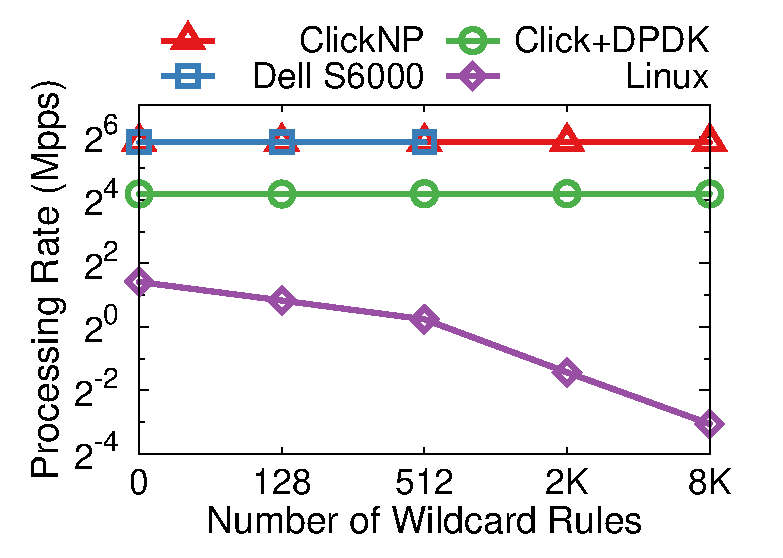
\includegraphics[width=0.5\textwidth]{eval/fw_1}
	}
	%	\subfloat[]{
	%		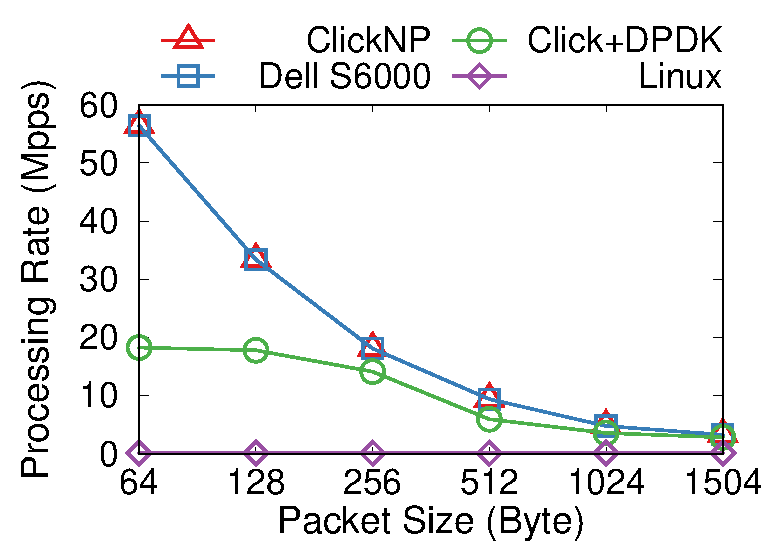
\includegraphics[width=0.225\textwidth]{eval/fw_2}
	%	}
	\subfloat[]{
		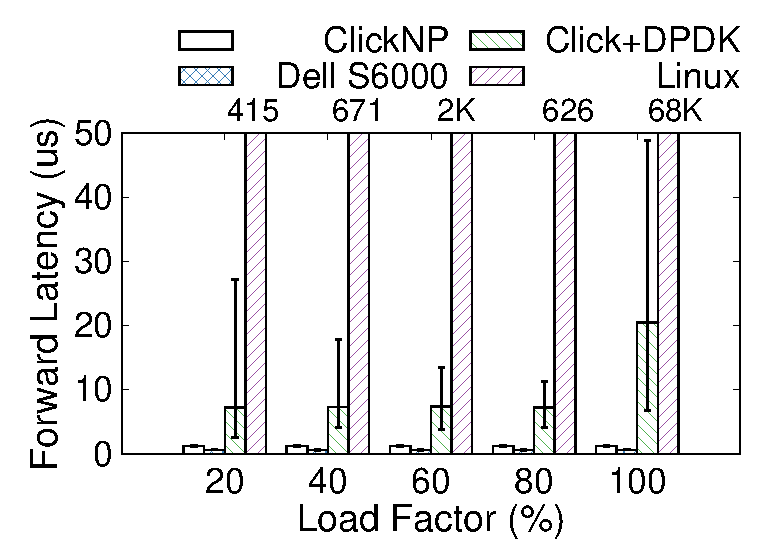
\includegraphics[width=0.5\textwidth]{eval/fw_3}
	}
	\hspace{1pt}
	\subfloat[]{
		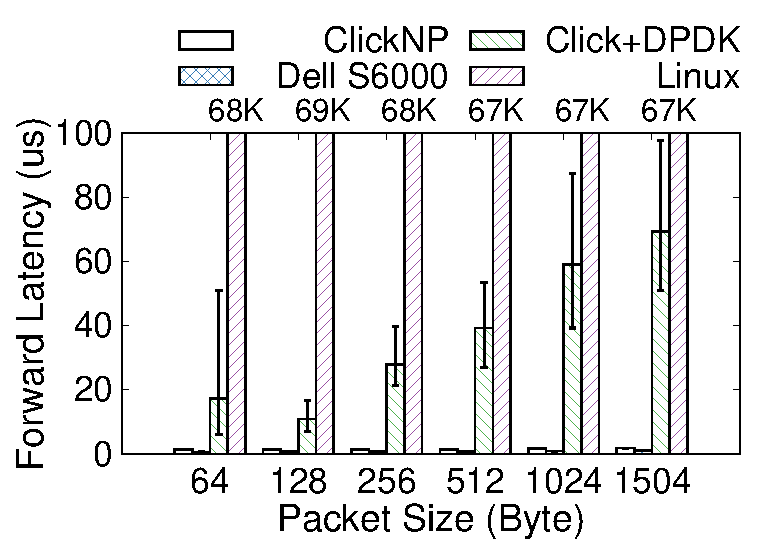
\includegraphics[width=0.5\textwidth]{eval/fw_4}
	}
	\subfloat[]{
		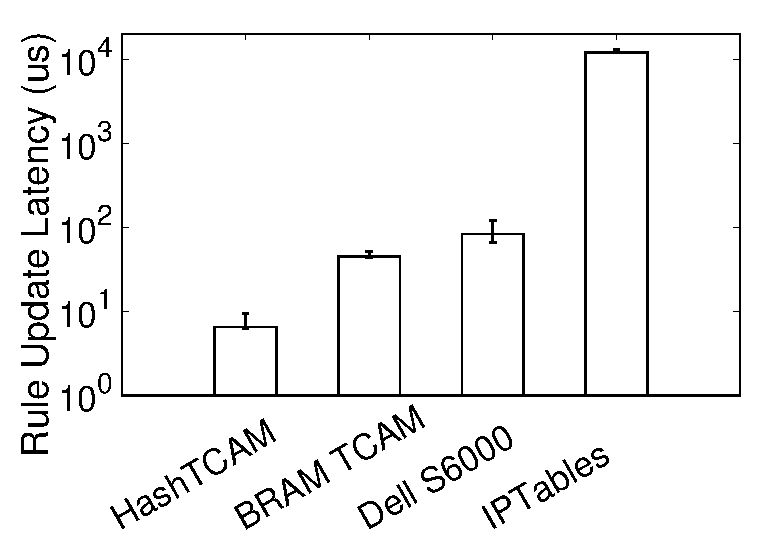
\includegraphics[width=0.5\textwidth]{eval/fw_5}
	}
	
	\caption{防火墙。误差条(error bar)表示 5\% 和 95\% 分位的延迟。在 (a) 和 (b) 图中,数据包大小为 64 字节。}
	
	\label{clicknp:fig:firewall}
\end{figure*}



\subsection{IPSec网关}
软件网络功能的一个问题是,当数据包需要一些计算密集型处理时,CPU很快就会成为瓶颈,例如,IPSec \cite {packetshader}。
IPSec数据面需要使用AES-256-CTR加密和SHA-1身份验证处理IPSec数据包。
如 \S \ref {clicknp:subsec:lib} 所示,单个AES\_CTR元件只能实现27.8~Gbps的吞吐量。因此,需要两个AES\_CTR元件并行运行以实现线速率。
然而,SHA-1很棘手。 SHA-1将数据包分成较小的数据块(64B)。
虽然一个数据块中的计算可以流水线化,但是一个IP数据包内的连续块之间存在依赖关系 - 下一个块的计算无法在前一个块完成之前开始!
如果按顺序处理这些数据块,吞吐量将低至1.07 Gbps。
幸运的是,可以利用不同数据包之间的并行性。
虽然当前数据包的数据块的处理仍在进行,但提供了不同数据包的数据块。
由于这两个数据块没有依赖关系,因此可以并行处理它们。
为了实现这一点,我们设计了一个名为 \textit {reservo} 的新元件(保留站的简称),它可以缓冲多达64个数据包,并为SHA-1元件调度独立的块。在计算了一个数据包的签名之后,\textit {reservo} 元件将它发送到将SHA-1 HMAC附加到数据包的下一个元件。
还有一件棘手的事情。
虽然SHA-1元件具有固定的延迟,但数据包的总延迟是不同的,即与数据包大小成比例。
当在SHA-1计算中调度多个分组时,这些分组可能是无序的,例如,大分组后面的较小分组可能更早地完成。
为了防止这种情况,在SHA-1元件之后进一步添加了一个\textit {reorder buffer}元件,该元件存储无序数据包并根据数据包的序列号恢复原始顺序。

下面比较IPSec 网关和StrongSwan~ \cite {strongswan},使用相同的密码套件AES-256-CTR和SHA1。
在单个IPSec隧道的情况下,图 \ref {clicknp:fig:IPSec}(a)显示了不同数据包大小的吞吐量。
对于所有规模,IPSecGW实现了线路速率,即64B数据包为28.8 Gbps,1500B数据包为37.8 Gbps。
然而,StrongSwan最多只能达到628 Mbps,随着数据包变小,吞吐量也会降低。
这是因为尺寸越小,需要处理的数据包数量就越多,
因此系统需要计算更多的SHA1签名。
图 \ref {clicknp:fig:IPSec}(b)显示了不同负载因子下的延迟。 同样,IPSecGW产生的恒定延迟为13 $\mu$s,
但是StrongSwan会产生更大的延迟和更高的方差,最长可达5 ms!



\begin{figure*}[htbp]
	\centering
	\subfloat[]{
		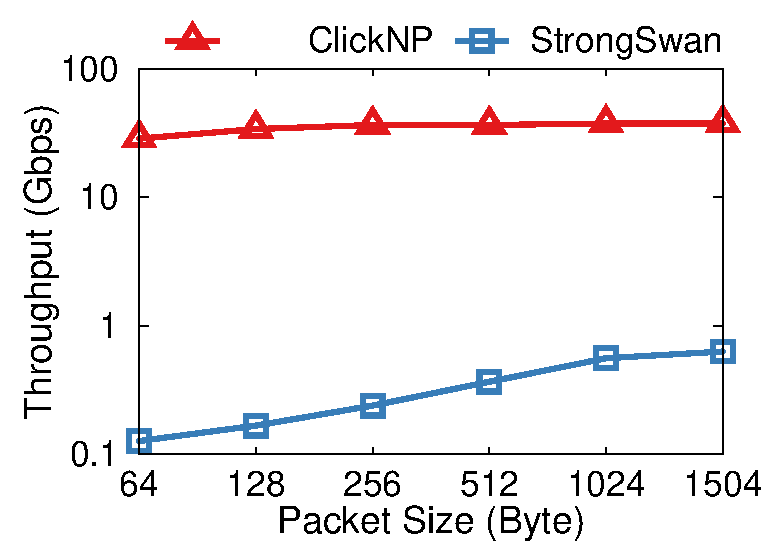
\includegraphics[width=0.5\textwidth]{eval/ipsec_1}
	}
	\subfloat[]{
		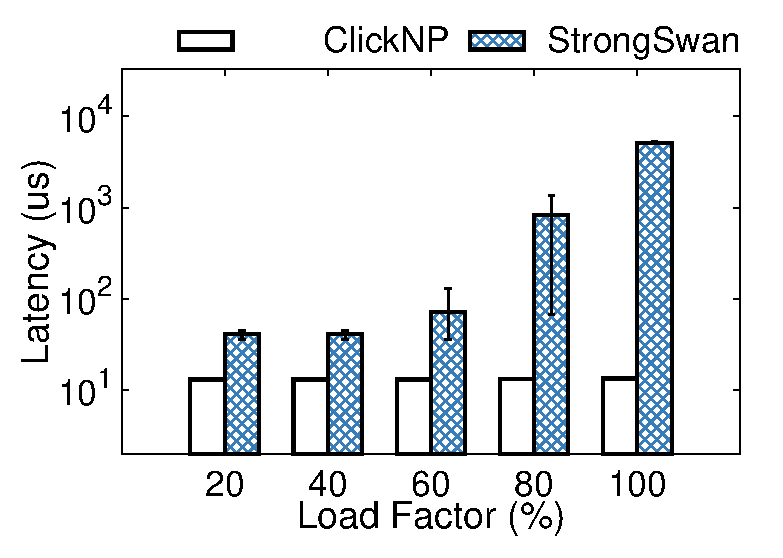
\includegraphics[width=0.5\textwidth]{eval/ipsec_2}
	}
	
	\caption{IPSec 网关。}
	
	\label{clicknp:fig:IPSec}
\end{figure*}



\subsection{L4负载平衡器}
L4 负载平衡器根据Ananta~ \cite {ananta}中的\textit {multiplexer}(MUX)实现。
MUX服务器基本上查看数据包标头,并查看是否已为该流分配了\textit {直接地址}(DIP)。
如果是,则通过NVGRE隧道将分组转发到由DIP指示的服务器。否则,MUX服务器将调用本地控制器为流分配DIP。
MUX服务器中需要按流状态。
由于存在故障并且避免黑洞需要即时更改后端服务器列表,因此无法使用基于散列的ECMP。此外,高级LB还可能需要负载感知平衡。
流表用于记录流向其DIP的映射。
为了处理数据中心的大流量,它需要L4LB在流表中支持多达3200万个流。
显然,如此大的流量表不能适应FPGA的BRAM,必须存储在板载DDR存储器中。
但是,访问DDR内存很慢。
为了提高性能,在BRAM中创建了一个带有16K高速缓存行的4路关联流缓存。最近最少使用(LRU)算法用于替换流缓存中的条目。

在本章的实现中,传入的数据包首先传递一个\textit {解析器}(parser)元件,该元件提取5元组并将它们发送到\textit {流缓存}(flow cache)元件。
如果在流缓存中找不到流,则将数据包的元数据转发到全局流表,该表读取DDR中的完整表。
如果仍然没有匹配的条目,则该数据包是流的第一个数据包,并且请求被发送到\textit {DIPAlloc}元件,以根据负载平衡策略为该流分配DIP。
确定DIP后,将一个条目插入到流表中。

在确定分组的DIP之后,封装元件将检索下一跳信息,例如IP地址和VNET ID,并相应地生成NVGRE封装的分组。
对于流的剩余分组,从流状态提取DIP。
如果收到FIN数据包或发生超时,则流条目将无效
在从流中接收任何新数据包之前。
在确定DIP之后,从BRAM检索下一跳元数据并封装NVGRE头以将分组引导到分配的DIP。

除了\textit {DIPAlloc}元件之外,所有元件都放在FPGA中。
由于只有流的第一个数据包可能会出现\textit {DIPAlloc}并且分配策略也可能很复杂,因此更适合运行
CPU上的\textit {DIPAlloc},是联合CPU-FPGA处理的另一个例子。



下面比较L4LB与Linux虚拟服务器(LVS) \cite {lvs}。
为了对系统进行压力测试,使用64B数据包生成大量并发UDP流,目标是一个虚拟IP(VIP)。
图 \ref {clicknp:fig:l4}(a)显示了具有不同并发流数的处理速率。
当并发流量小于8K时,L4LB达到51.2Mpps的线路速率。
但是,当并发流的数量变大时,处理速率开始下降。
这是因为L4LB中的流缓存未命中。
当流缓存中缺少流时,L4LB必须访问板载DDR内存,
这会导致性能下降。
当流量太多时,例如32M,缓存未命中占主导地位且对于大多数数据包而言,
L4LB需要一次访问DDR内存。因此处理速度降低到11Mpps。
在任何情况下,LVS的处理速率都很低。
由于LVS将VIP关联到仅一个CPU核心,因此其处理速率必须达到200Kpps。

图 \ref {clicknp:fig:l4}(b)显示了不同负载条件下的延迟。
在这个实验中,将并发流的数量修复为100万。
可以看到,L4LB实现了4 $\mu$s 的非常低的延迟。
然而,LVS会导致约50 $\mu$s 的延迟。
当提供的负载高于100Kpps时,这种延迟会迅速上升,超过LVS的容量。

最后,图 \ref {clicknp:fig:l4}(c)比较L4LB和LVS接受新流的能力。
这个实验指示PktGen生成尽可能多的单包微流。
可以看到,L4LB每秒可以接受高达10M的新流量。
由于单个PCIe插槽每秒可以传输16.5M的传输,因此瓶颈仍然是DDR访问。
\textit {DIPAlloc} 元件只是以循环方式分配DIP。
对于复杂的分配算法,\textit {DIPAlloc} 的CPU核心将成为瓶颈,并且可以通过在更多CPU核心上复制 \textit {DIPAlloc} 元件来提高性能。
对于LVS,由于数据包处理能力有限,它每秒最多只能接受75K个新连接。


\begin{figure*}[htbp]
	\centering
	
	\subfloat[]{
		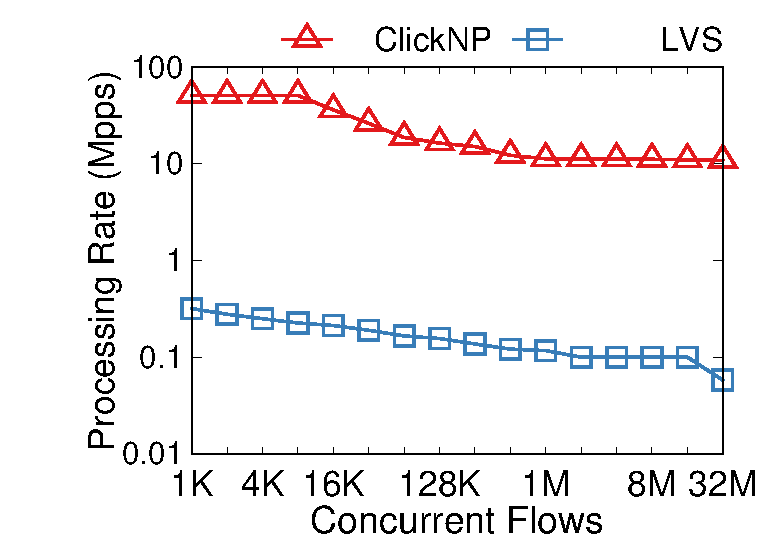
\includegraphics[width=0.5\textwidth]{eval/l4_2}
	}
	\subfloat[]{
		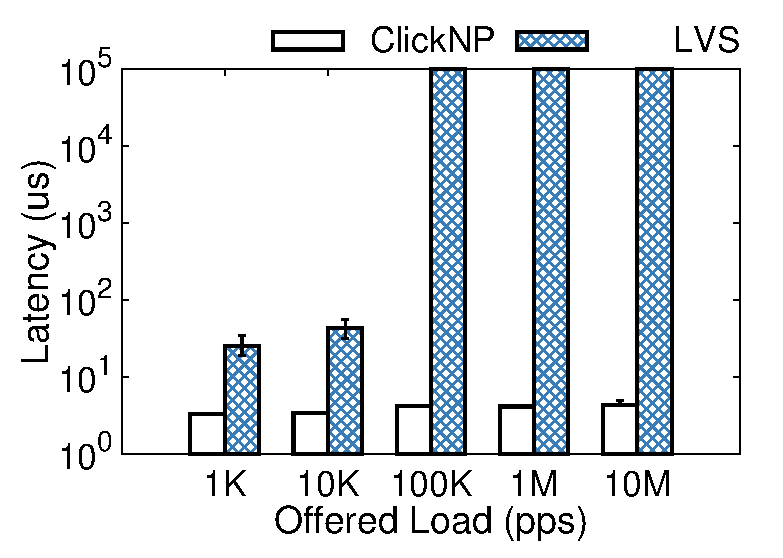
\includegraphics[width=0.5\textwidth]{eval/l4_1}
	}
	
	\subfloat[]{
		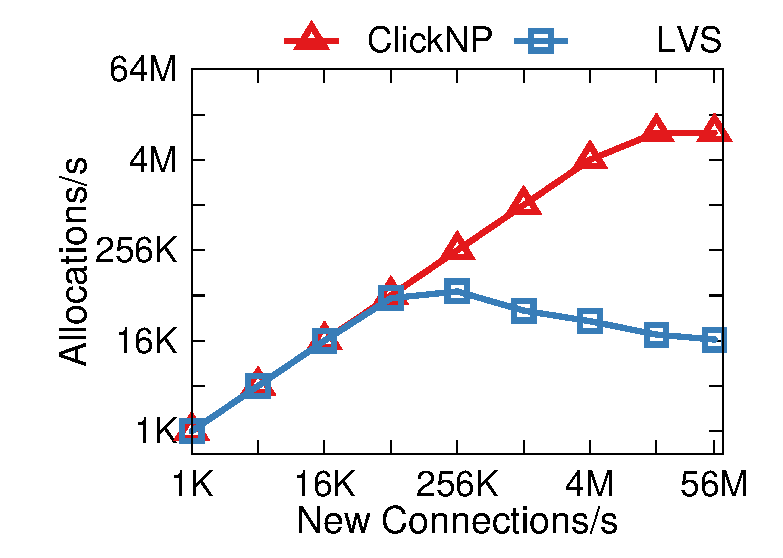
\includegraphics[width=0.5\textwidth]{eval/l4_3}
	}
	
	\caption{L4 负载均衡器的性能评估。}
	\label{clicknp:fig:l4}
	
\end{figure*}


\subsection{pFabric 流调度器}


\name 也是网络研究的好工具。
由于灵活性和高性能,\name 可以快速制作最新研究的原型并将其应用于真实环境。

本节使用\name 来实现一个最近提出的数据包调度规则--pFabric \cite {pfabric}。
pFabric调度很简单。它只保留浅缓冲区(32个数据包),并始终使具有最高优先级的数据包出列。当缓冲区已满时,优先级最低的数据包将被丢弃。
pFabric显示在数据中心中实现接近最佳的流完成时间。
在原始论文中,作者提出使用二进制比较树(Binary Comparison Tree,BCT)来选择具有最高优先级的数据包。
但是,虽然BCT只需要$O(log_2 N)$个周期来计算最高优先级的数据包,但在连续的选择过程之间存在依赖关系。这是因为只有当前一个选择完成后才能知道最高优先级的数据包,然后才能可靠地启动下一个选择过程。
这种限制要求时钟频率至少为300MHz才能实现40Gbps的线速,这对当前的FPGA平台来说是不可能的。
本文使用不同的方式来实现pFabric调度程序,它更容易并行化。
该方案基于\textit{移位寄存器优先级队列}(shift register priority queue) \cite {moon2000scalable}。
条目以非增加优先级顺序保存在$K$个寄存器中。
出列时,所有条目都向右移动并弹出头部。这只需要1个周期。
对于入队操作,新数据包的元数据将转发到所有条目。
现在,对于每个条目,可以在条目中的分组,新分组和相邻条目中的分组之间执行本地比较。
由于所有局部比较都可以并行进行,因此入队操作也可以在1个周期内完成。
入队和出队操作可以进一步并行化。
因此,可以在一个周期中处理分组。

例如,可以使用\name 轻松实现pFabric调度程序\cite {pfabric},并将其应用于本文的测试平台。
本实验修改了一个软件TCP流生成器\cite {mqecn},以便在数据包有效负载中放置流优先级,即流的总大小。
本实验根据\cite {pfabric}中的数据挖掘工作负载生成流,并使用\textit {RateLimit}元件将限制出口端口进一步设置为10~Gbps。
应用pFabric根据流优先级调度出口缓冲区中的流量。
图 \ref {clicknp:fig:pfabric}显示了pFabric,具有Droptail队列的TCP的平均流完成时间(FCT)和理想值。
该实验验证了pFabric在这种简单的场景中实现了接近理想的FCT。

\begin{figure}[h!]
	\centering
	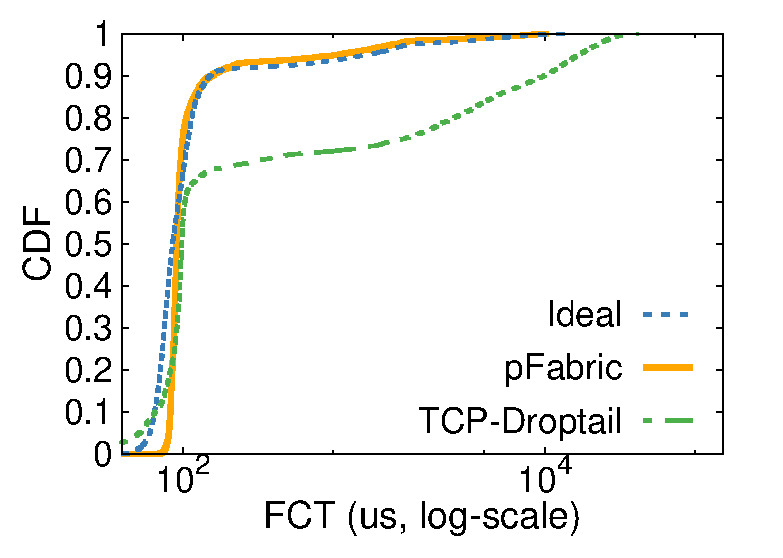
\includegraphics[width=0.6\textwidth]{eval/pfabric}
	\caption{pFabric 的验证。}
	\label{clicknp:fig:pfabric}
\end{figure}

\subsection{容错的 LTE SPGW}

\subsection{端口扫描检测}

\subsection{HTTPS RSA 加速}

\subsection{正则表达式匹配}

\subsection{神经网络推理}

\egg{
\textbf{Stateful L4 load balancer.} We compare our ClickNP implementation with Linux Virtual Server (LVS) \cite{lvs} using both real-world traffic trace on a L4 load balancer \cite{gandhi2014duet} and synthetic traces to simulate adversary scenarios.
The real-world trace contains 1.3M flows collected in two hours with 26Gbps average throughput and 45KB median flow size.
The first adversary trace is round-robin scheduling packets from a large number of infinite UDP flows with 64B packet size to stress the load balancer under high concurrency.
The second adversary trace is a lot of tiny UDP flows to test how many new connections the load balancer can process per second.

Figure \ref{clicknp:fig:l4} shows that ClickNP L4 load balancer has 50\approx500x lower latency than LVS on real-world trace, supports 32M concurrent flows and able to accept \approx10M new flows per second.
This performance is comparable to high-end hardware load balancers \cite{f5loadbalance}, while ours have low cost and high flexibility.
Figure \ref{clicknp:fig:l4} also shows the importance of SRAM cache and pipelined DRAM access.
Our board can perform at most 13.6M DRAM random reads per second, and our new flow allocation rate gets near this limit thanks to pipelined DRAM access.
}

\egg{
First we test the performance under real-world data center traffic. We adopted the same traffic trace as DUET\cite{}, and picked the first ten minutes as testing data. Figure \ref{clicknp:fig:l4} shows the four experiments we performed on the L4 load balancer. We first use TCP traffic to evaluate the flow completion time (FCT) under different throughputs. Then we use UDP traffic to evaluate the latency. 

Next we tested the performance with adversary traffic to thest the worst case performance. We fixed every flow to be one 1504 byte packet, and test the throughput under different flow numbers, and latency under different new flow rates.
}

\section{讨论:资源利用率}

\egg{
	To evaluate ClickNP's area cost overhead compared to hand-written 硬件描述语言, we implemented several ClickNP elements resembling network functions in NetFPGA 10G \cite{netfpga} reference router and Openflow switch projects.
	Table \ref{clicknp:tab:netfpga} compares ClickNP's relative area cost over NetFPGA using Vivado 高层次综合 2015.4 and Altera OpenCL 15.1.
	Most ClickNP implementations show less than 100\% logic overhead and less than 30\% BRAM overhead. For tiny elements (\eg IP checksum), a fixed element overhead dominates.
}



本节将评估\name 网络功能的资源利用率。
表 \ref {clicknp:tab:applications} 总结了结果。
除了使用大多数BRAM来保存编码书的IPSec网关之外,所有其他网络功能仅使用中等资源(5 至 50 %)。
仍有空间容纳更复杂的网络功能。


\begin{table}[htbp]
	\centering
	\caption{ClickNP 网络功能汇总。}
	\label{clicknp:tab:applications}
	\small
	\begin{tabular}{l|r|r|r|r}
		\toprule
		Network Function & LoC$^\dagger$ & \#Elements & LE & BRAM \\
		\midrule
		\egg{
			Pkt generator & 13 & 6 & 16\% & 12\% \\
			Pkt capture & 12 & 10 & 8\% & 5\% \\
			OpenFlow firewall & 23 & 7 & 32\% & 54\% \\
			IPSec gateway & 37 & 10 & 35\% & 74\% \\
			L4 load balancer & 42 & 13 & 36\% & 38\% \\
			pFabric scheduler & 23 & 7 & 11\% & 15\% \\
		}
		Pkt generator & 665 & 6 & 16\% & 12\% \\
		Pkt capture & 250 & 11 & 8\% & 5\% \\
		OpenFlow firewall & 538 & 7 & 32\% & 54\% \\
		IPSec gateway & 695 & 10 & 35\% & 74\% \\
		L4 load balancer & 860 & 13 & 36\% & 38\% \\
		pFabric scheduler & 584 & 7 & 11\% & 15\% \\
		\bottomrule
		\multicolumn{5}{l}{$^\dagger$ 所有元件描述语言的代码行数与配置文件的行数之和。}
	\end{tabular}
\end{table}



接下来研究 \name 的细粒度模块化的开销。
由于每个元件都将生成逻辑块边界并仅使用FIFO缓冲区与其他块进行通信,因此应该存在开销。
为了衡量这种开销,创建一个只将数据从一个输入端口传递到输出端口的简单``\textit{空}''元件。
此\textit {空}元件的资源利用率应该很好地捕获模块化的开销。
不同的高层次综合工具可能使用不同数量的资源,但都很低,最小值为0.15%,最大值为0.4%。
因此,由于模块化,名称产生的开销很小。

最后研究\name 与手写硬件描述语言相比生成的硬件描述语言代码的效率。
为此,使用NetFPGA \cite {netfpga}作为参考。
首先,提取NetFPGA中的关键模块,这些模块由经验丰富的Verilog程序员进行了优化,
并在\name 中实现具有相同功能的对应元件。
然后,使用不同的高层次综合工具作为后端,比较这两种实现之间的相对面积成本。
结果总结在表 \ref {clicknp:tab:netfpga} 中(见本章末尾的全页表)。
由于不同的工具可能具有不同的面积成本,因此记录最大值和最小值。
可以看到,与手工优化代码相比,自动生成的硬件描述语言代码使用更多区域。
然而,差异并不是很大。
对于复杂模块(如表格顶部所示),相对面积成本小于2倍。
对于微小模块(如表格底部所示),相对面积成本看起来更大,但绝对资源使用量很小。
这是因为所有的高层次综合工具都会产生一个固定的开销,占据微小模块的面积成本。


\begin{table}[htbp]
	\centering
	\caption{相比 NetFPGA 的面积开销。}
	\label{clicknp:tab:netfpga}
	\small
		\begin{tabular}{l|r|r|r}
			\toprule
			\multirow{2}{2.2cm}{NetFPGA 功能} & 逻辑查找表(LUT) & 寄存器 & 内存(BRAM) \\
			& 最小 / 最大 & 最小 / 最大 & 最小 / 最大 \\
			\midrule
			输入选择器  & 2.1x / 3.4x & 1.8x / 2.8x & 0.9x / 1.3x \\
			输出队列   & 1.4x / 2.0x & 2.0x / 3.2x & 0.9x / 1.2x \\
			数据包头解析器  & 0.9x / 3.2x & 2.1x / 3.2x & N/A \\
			Openflow 查找表 & 0.9x / 1.6x & 1.6x / 2.3x & 1.1x / 1.2x \\
			\midrule
			\midrule
			IP 校验和计算    & 4.3x / 12.1x & 9.7x / 32.5x & N/A \\
			隧道封装          & 0.9x / 5.2x & 1.1x / 10.3x & N/A \\
			\bottomrule
		\end{tabular}
\end{table}

总之,\name 可以为FPGA生成高效的硬件描述语言,只需要适度的面积成本,可以构建实用的网络功能。
展望未来,FPGA技术仍在迅速发展。例如,Intel的Arria 10 FPGA 和最新的 Stratix 10 FPGA 的面积分别是本文使用的芯片(Stratix V)的 2.5 倍和 10 倍。
因此,高层次综合的面积成本将来将受到较少的关注。


\egg{
Figure \ref{clicknp:tab:applications} shows Logic Elements (LE) and BRAM footprint of aforementioned ClickNP applications.
Catapult shell and OpenCL runtime take 30\% LEs and 18\% BRAMs in addition to ClickNP applications.
}


\egg{
Original data:
Function	LUTs			Registers			BRAMs		
NetFPGA	AOCL	V高层次综合	NetFPGA	AOCL	V高层次综合	NetFPGA	AOCL	V高层次综合
Input arbiter	2048	4346	6998	4553	12843	8348	30	40	26
Output queue	3824	5280	7542	6479	13409	21005	22.5	26	20
Header parser	626	2012	567	698	6095	817	N/A		
Openflow table	3923	6322	3535	4438	10171	7140	33.5	40	38
IP checksum	207	2511	884	162	5269	1576	N/A		
Encap	684	3536	636	821	8493	871	N/A	
}

\egg{
\subsection{Network Benchmark Suite}

\subsubsection{Configurable Flow Generator}

\begin{lstlisting}
Rand(0,1,2) -> MetaGen(1,1) -> RevParser(1,1) -> IPChecksum(1,1) -> TCPChecksum(1,1) -> NVGRE_Encap(1,1) -> tor_out
\end{lstlisting}

\subsubsection{Packet Trace Replay}

\begin{figure}[h!]
	\centering
	
\includegraphics[width=0.6\columnwidth]{image/logo}
	\vspace{-0.15in}
	\caption{Traffic Replay Throughput, x: packet size, y: Gbps, lines: ClickNP, CPU}
	\vspace{-0.15in}
	\label{clicknp:fig:TrafficReplayPerformance}
	%    
\end{figure}

\subsubsection{Traffic Monitor}

\begin{lstlisting}
tor_in -> Receiver -> Drop (1,0)
\end{lstlisting}

latency, throughput, sequence number check

\subsection{Network Virtualization}

\subsubsection{NVGRE Tunneling}

\begin{figure}[h!]
	\centering
	
\includegraphics[width=0.6\columnwidth]{image/logo}
	\vspace{-0.15in}
	\caption{Tunnel Encap + Decap Performance, x: packet size, y: Gbps, lines: ClickNP, Hyper-V}
	\vspace{-0.15in}
	\label{clicknp:fig:NVGREPerformance}
	%    
\end{figure}

\subsubsection{Per-VM Metering and Rate Limiting}

\subsection{Security}

\subsubsection{Network-layer Firewall}

\begin{lstlisting}
Parser :: parser(1,2)
DropPolicer :: action(2,2)
tor_in -> parser[1] -> [1]action[1] -> nic_out
parser[2] -> ExtractFiveTuple(1,1) -> Hashtable @(1,1) -> [2]action[2] -> Drop (1,0)
\end{lstlisting}

\begin{figure}[h!]
	\centering
	
\includegraphics[width=0.6\columnwidth]{image/logo}
	\vspace{-0.15in}
	\caption{Network-layer Firewall Performance, x: \#rules, y: pps, lines: ClickNP, Linux iptables}
	\vspace{-0.15in}
	\label{clicknp:fig:FirewallPerformance}
	%    
\end{figure}

\subsubsection{Application-layer Firewall}

\begin{lstlisting}
Parser :: parser(1,2)
DropPolicer :: action(2,2)
tor_in -> parser[1] -> [1]action[1] -> nic_out
parser[2] -> ExtractFiveTuple(1,1) -> RegexMatch @(1,1) -> [2]action[2] -> Drop (1,0)
\end{lstlisting}

\begin{figure}[h!]
	\centering
	
\includegraphics[width=0.6\columnwidth]{image/logo}
	\vspace{-0.15in}
	\caption{Application-layer Firewall Performance, x: \#rules, y: Gbps, lines: ClickNP, snort \cite{roesch1999snort}}
	\vspace{-0.15in}
	\label{clicknp:fig:WAF_Performance}
	%    
\end{figure}

\subsubsection{DDoS Detection with Bitmap Sketch}

\begin{lstlisting}
Parser :: parser(1,2)
tor_in -> parser[1] -> nic_out
parser[2] -> ExtractVMID(1,1) -> HashTable @(1,1) -> ExtractSrcIP(1,1) -> BitmapSketch @(1,1) -> Drop (1,0)
\end{lstlisting}

OpenSketch \cite{yu2013software}

\begin{figure}[h!]
	\centering
	
\includegraphics[width=0.6\columnwidth]{image/logo}
	\vspace{-0.15in}
	\caption{Sketch Accuracy, x: \#real flows, y: relative error (\%) with error bar}
	\vspace{-0.15in}
	\label{clicknp:fig:SketchAccuracy}
	%    
\end{figure}


\subsection{Scheduling}

\subsubsection{PIAS Tagging}

PIAS \cite{bai2014pias}

\subsubsection{Generic Priority Queue}

pFabric \cite{alizadeh2013pfabric}

\subsubsection{Packet Pacing}

Silo \cite{jang2015silo}

\begin{figure}[h!]
	\centering
	\includegraphics[width=0.6\columnwidth]{image/logo}
	\vspace{-0.15in}
	\caption{CDF of pacing inaccuracy due to buffer overflow, x: percentile, y: time shift, lines: buffer sizes}
	\vspace{-0.15in}
	\label{clicknp:fig:PacingAccuracy}
	%    
\end{figure}

\subsubsection{Timestamping}

TIMELY \cite{mittal2015timely} measures RTT as the signal for congestion control. It requires both receive and send timestamping feature and hardware-generated ACK of recent 网卡s. Furthermore, since ACKs have already been sent by 网卡 hardware, OS networking stack needs modifications to avoid generating duplicate ACKs.

With ClickNP we can do the same latency measurement without using a 网卡 with timestamping feature, and does not require modification to the OS networking stack, as long as the FPGAs at sender and receiver have same clock frequency. The idea is to subtract the latency spent in receiver-side OS networking stack. Upon reception of a data packet, we subtract the timestamp and expects the OS to echo back the timestamp in the ACK packet. When the ACK packet is sent, we add the timestamp, as if we had shifted the initial timestamp by OS processing latency. Pseudo code:

\begin{lstlisting}
.element SendTimestamp {
    .state { uint timestamp = 0; }
    .handler {
        if (input_ready) {
            if (!is_ack_packet())
                set_tsval (timestamp);
            else
                set_tsecr (get_tsecr() + timestamp);
        }
        timestamp ++;
    }
}
.element RecvTimestamp {
    .state { uint timestamp = 0; }
    .handler {
        if (input_ready) {
            if (!is_ack_packet())
                set_tsval (get_tsval() - timestamp);
            else
                set_tsval (timestamp);
        }
    }
}
nic_in -> Parser (1,2) -> SendTimestamp (2,1) -> tor_out
tor_in -> Parser (1,2) -> RecvTimestamp (2,1) -> nic_out
\end{lstlisting}

\begin{figure}[h!]
	\centering
	\includegraphics[width=0.6\columnwidth]{image/logo}
	\vspace{-0.15in}
	\caption{CDF of measured RTT, x: percentile, y: RTT, lines: hardware ACK (ideal), remove OS latency (close to ideal), not remove OS latency (poor)}
	\vspace{-0.15in}
	\label{clicknp:fig:TimestampAccuracy}
	%    
\end{figure}
}

\egg{
Figure~\ref{clicknp:fig:trafficgen} shows the throughput of \name\ traffic generator and capture. We can see that the generator can
generate packets at line-rate of 40 Gbps. 
When packet size is small ($<256B$), the measured throughput is slightly less than 40 Gbps. We confirm this is due to a
bug in Ethernet MAC in the shell, which may drop a few flits when packet rate is high. 
Figure~\ref{clicknp:fig:trafficgen}(b) shows the capture performance in packet per second.  

\begin{figure}[htbp]
	\centering
	\subfloat[] {
	\includegraphics[width=0.225\textwidth]{eval/trafficgen}
	}
	\subfloat[] {
	\includegraphics[width=0.225\textwidth]{eval/dump}
	}
	
	\caption{(a) Traffic generator. (b) Traffic capture.}
	\label{clicknp:fig:trafficgen}
\end{figure}
}
\egg{
In this section we evaluate throughput and latency of applications presented in section \ref{clicknp:sec:application}. All these application can achieve line-rate throughput and microsecond-scale latency for reasonable traffic patterns. Latency is averaged over $1000$ rounds, and error bars mark the $5\%$ and $95\%$ percentile.

\textbf{Traffic generator.} We use our traffic generator to send packets to 网卡, and use Windows Performance Monitor to measure the throughput. As shown in Figure \ref{clicknp:fig:trafficgen}, our generator is able to generate packets at 40Gbps line rate when the packet size is not less than 256 bytes. The small gap for 64-byte packets is due to lack of back-pressure in 40GbE MAC of FPGA shell.

\textbf{Traffic capture.} We evaluate the throughput of dumper and results are presented in \ref{clicknp:fig:dump}.
Each host kernel runs on a separate core and traffic is split evenly to kernels by flow tuple hash.
With four host elements receiving the packets, we can approximately achieve the maximum speed of the PCIe channel.
When we only need the flow tuple and timestamp, ClickNP can easily capture line rate with two cores.
}

\egg{
\textbf{IPSec gateway.} We use StrongSwan \cite{strongswan} with AES256CTR + SHA1 IKEv2 cipher suite as baseline.
After setting up IPSec keys and nonces in ClickNP elements via signal, we send UDP packets in a single IPSec tunnel to test throughput and latency on encryption path.
StrongSwan leverages only one CPU core due to tunnel message sequencing.
As shown in Figure \ref{clicknp:fig:IPSec}, \textit{Reservo} to exploit packet-level parallelism for SHA-1 element shows 40x performance gain compared to unoptimized version. }

\egg{
\textbf{OpenFlow firewall.} We compare our firewall with Click + DPDK \cite{barbette2015fast} on 4 cores, and Linux iptables (for wildcard match) / ipset \cite{ipset} (for exact match) with RSS on 8 cores.
We also include Dell S6000, a high-end commodity switch, as a reference.

We optimized FromDPDKDevice element in Click to enable receiving packets on multiple cores, while the bottleneck becomes Mellanox polling-mode driver at 18 Mpps.
Click uses a radix tree for exact IP lookup and a classification tree for wildcard flow tuple lookup, so table lookup is not bottleneck of Click.
Linux ipset uses hash table for exact lookup. Linux iptables match wildcard rules linearly, which is the source of low throughput and high latency.
Dell S6000 supports 1.7K 5-tuple wildcard match rules.
For all packet sizes and number of rules, ClickNP offers line rate throughput and latency comparable to commodity ASIC.

Additionally, for 8K wildcard rules, Click takes minutes to generate the classification tree and cannot offer live rule update. ClickNP can perform 350K live rule updates per second while the data plane keeps line forwarding rate. Dell S6000 can perform 12K live rule updates per second.

16K exact, 8 K wild.
}

\egg{
All results are presented in Figure \ref{clicknp:fig:firewall}. The first two subfloats are to show how packet size and rule numbers influence throughput. In the first subfloat, the packet size is fixed at 64 byte. And in the second subfloat, the numbers of rules is set to be 64k(exact)/8k(wild).

The last two subfloats are about latency. In \ref{clicknp:}, we fixed the packet size to be ?? and evaluated the latency with different loads. In \ref{clicknp:}, we change the packet size to see how the latency changes in maximum load scenario. 

From all these figures we can see that ClickNP approximates the performance of Dell S6000, and has a ???x boost on the CPU solution.
}

\section{连接数可扩放的 RDMA 网卡实现}
\label{socksdirect:sec:discussion}


\begin{figure}[htbp]
	\centering
	\includegraphics[width=0.9\textwidth]{images/scalable_rdma.pdf}	
	\caption{基于可编程网卡的连接数可扩放 RDMA。}
	\label{socksdirect:fig:scalable-rdma}
\end{figure}

%\textbf{Communicating with TCP/IP peers.}
%We use a user-space networking stack to communicate with regular TCP/IP peers, but the compatibility may be limited~\cite{yasukata2016stackmap}.
%To solve this problem, after receiving the TCP SYN+ACK, the monitor can create an established kernel TCP connection using TCP connection repair~\cite{tcp-connection-repair}.
%Moreover, if the application and monitor share a network namespace, the monitor can send the kernel FD to the application via Unix domain socket, then \libipc{} can use the FD without delegation to the monitor.

%\textbf{Connecting to many RDMA capable hosts.}
%With a lot of hosts, the 网卡 still suffer from performance degradation due to large number of connections.
%In contrast, user-space networking stack alleviates this problem because the 网卡 is stateless.
%We provide a socket option to enable applications to delegate operations to the monitor and use user-space networking stack even if the peer supports RDMA.
%An application can choose to use RDMA for latency sensitive and throughput demanding connections, and user-space networking stack for others.

\parab {扩放到大量连接。}
\sys {}对许多连接的可伸缩性受SHM和RDMA的限制。
为了表明\libipc {}和监视器不是瓶颈,我们运行一个综合实验,在两个重用RDMA QP和SHM的进程之间创建了很多连接。使用\libipc {}的应用程序线程每秒可以创建1.4~M个新连接,这是Linux的20倍和mTCP的2倍 \cite {jeong2014mtcp}。监视器每秒可以创建5.3~M个连接。

由于主机内的进程数量有限,因此SHM连接的数量可能不会很大。
但是,一台主机可能连接到许多其他主机,RDMA的可扩展性成为一个问题。
这归结为两个问题。
首先,RDMA 网卡使用网卡内存作为缓存来保持每个连接状态。有数千个并发连接,性能受到频繁缓存未命中的影响 \cite {mprdma,kaminsky2016design,kalia2018datacenter}。
但是,网卡配备了小内存,因为RDMA传统上部署在中小型集群中。
随着近年来大规模的RDMA部署 \cite {guo2016rdma},商品网卡拥有更大的内存来存储数千个连接 \cite {kalia2018datacenter}而Smart网卡拥有千兆字节的DRAM~ \cite {mellanox-innova,mellanox-bluefield,smartnic}。
我们相信未来的数据中心不会担心网卡缓存未命中问题。
第二个问题是在我们的测试平台中建立RDMA连接需要大约 $30 \mu s$,这对于短连接很重要。但是,此过程仅涉及本地CPU和网卡之间的通信,我们希望未来的工作能够得到改进。

%Another promising direction to solve the RDMA concurrency issue is to implement the reliable transport in CPU, and the 网卡 remains stateless. However, RDMA UD does not support one-sided write, so the ring buffer in Sec.~\ref{socksdirect:subsec:lockless-queue} will not work. Existing software RDMA~\cite{soft-roce} has low performance. It would be interesting to co-design software and 网卡.

\textbf {RDMA的QoS。}
我们将数据平面性能隔离和拥塞控制卸载到RDMA网卡上,遵循新的工作方式 \cite {peter2016arrakis,zhu2015congestion,lu2017memory,mprdma,mittal2018revisiting}这个方向,因为数据中心的网卡正变得越来越可编程  \cite{smartnic,cavium,kaufmann2015flexnic,mellanox-innova,mellanox-bluefield},公有云已经在虚拟机之外的网络功能中提供QoS了\cite {li2016clicknp,panda2016netbricks,floem-osdi18}。

%\textbf{Networking stack on other layers.}
%RDMA: lower layer,
%eRPC, message queue, etc: higher layer.

%\section{Related Work}
%\label{socksdirect:sec:related-work}

%Several mostly related works have been discussed in Sec.~\ref{socksdirect:subsec:related-work}.

\iffalse
\parab{Linux kernel optimization.}
One line of research optimizes the kernel stack for higher socket performance. FastSocket~\cite{lin2016scalable} and Affinity-Accept~\cite{pesterev2012improving} scale connection creation to multiple cores, but synchronization is still needed when multiple threads share a socket.
FlexSC~\cite{soares2010flexsc} proposes exception-less system calls to reduce kernel crossing overhead.
Zero-copy socket~\cite{thadani1995efficient,chu1996zero} still needs copy-on-write on senders.
In addition, they fail to remove cache miss and transport overheads.


\parab{New OS stacks.}
Another line of research proposes new OS stacks with modified socket interface, mostly aiming at zero copy and fast event notification. Existing socket applications need modifications to use the new interfaces.
For intra-server connections, Arrakis~\cite{peter2016arrakis} and IX~\cite{belay2017ix} use the 网卡 to forward packets from one process to another. The hairpin latency from CPU to 网卡 is at least two PCIe delays, which is one order of magnitude higher than inter-core cache migration delay. In addition, the data plane switching throughput of a 网卡 is constrained by PCIe bandwidth (Figure~\ref{socksdirect:fig:eval-corenum-tput}).

For inter-server connections, most OS stacks implement transport in software. IX~\cite{belay2017ix} and Stackmap~\cite{yasukata2016stackmap} run in the kernel to enforce QoS policy or preserve protocol compatibility with Linux, while Arrakis~\cite{peter2016arrakis} and SandStorm~\cite{marinos2014network} run in user mode to maximize performance.
RDMA and transport virtualization~\cite{tsai2017lite,niu2017network} also enforce QoS in the hypervisor.
Due to the additional level of indirection, kernel stacks cannot remove kernel crossing, while batched syscalls add latency.
Further, large-scale deployment of kernel-based stacks is more complicated than user-space libraries~\cite{andromeda}.
\sys offloads transport and QoS to 网卡 hardware.
RDMA transport has been deployed in many data centers~\cite{guo2016rdma}, and an emerging line of work~\cite{zhu2015congestion,lu2017memory,mprdma} improves congestion control and QoS in large-scale RDMA deployments.
For flexibility, programmable 网卡s are being adopted in data centers~\cite{smartnic,cavium}, as they are more efficient than general-purpose CPUs for network processing~\cite{kaufmann2015flexnic,li2016clicknp}.



\parab{User-space socket.}
A third line of research runs socket in user space.
mTCP~\cite{jeong2014mtcp}, Seastar~\cite{seastar}, 
F-stack~\cite{fstack} and LOS~\cite{huang2017high} use a high performance packet I/O framework (\textit{e.g.} netmap~\cite{rizzo2012netmap}, DPDK~\cite{dpdk} and PF\_RING~\cite{pf-ring}) and achieves compatibility with most Linux socket functions and scalability with number of cores and sockets.
LibVMA~\cite{libvma}, OpenOnload~\cite{openonload} and DBL~\cite{dbl} are fully compatible with existing applications. However, they use vendor-specific 网卡 features and do not scale to multiple threads or connections.
In addition, user-space sockets do not support zero copy or efficient multitasking.

Most user-space sockets focus on inter-server and do not optimize for intra-server connections.
FreeFlow~\cite{freeflow} uses shared memory for intra-server communication and RDMA for inter-server, but it provides an RDMA interface.
Existing socket to RDMA translation approaches, \textit{e.g.} SDP~\cite{socketsdirect} and rsockets~\cite{rsockets} are not fully compatible with Linux and do not address scalability challenges.


%\parab{RDMA.}
%First, RDMA is not suitable for WAN. Second, RDMA has scalability issue when one server connects to many servers. Software transport in CPU access connection states in host memory, while hardware RDMA transport caches connection states in 网卡 and swaps out to host memory when cache overflows. First, CPU cache miss costs less than 0.1$\mu$s, while 网卡 cache miss costs 0.5$\mu$s~\cite{kaminsky2016design}. Second, CPU memory bandwidth is an order of magnitude larger than 网卡 PCIe bandwidth. In light of this, a host should switch to software transport when it actively communicates with a large number of hosts. Fortunately, Modern 网卡s has an increasing size of memory and supports more active connections without performance degradation~\cite{kaminsky2016design}.
\fi


\iffalse
\begin{itemize}
	\item New abstraction (RDMA, lwip + DPDK etc.) 
	\begin{itemize}
		\item 
	\end{itemize}
	\item Compatible with socket (libvma, LOS etc.) 
	\begin{itemize}
		\item Violate goal 2: memory copy 
		\item Violate goal 3: thread synchronization for multi-thread applications 
	\end{itemize}
	\item Common problems: 
	\begin{itemize}
		\item Designed for networking, does not support or optimize for IPC communication inside the same server 
		\item Violate goal 4: Not optimized for many connections 
	\end{itemize}
\end{itemize}
\fi


%%!TEX root=main.tex
\section{Future Work}
\label{clicknp:sec:future}

One challenge for deploying ClickNP in production data centers is 30-second interruption of data plane while FPGA is being reprogrammed. Partial reconfiguration \cite{bourgeault2011alteras} feature of FPGA can be utilized to keep basic packet forwarding functionality while FPGA is being reprogrammed.

On-chip DRAM has relatively low throughput which is insufficient for rule caching and line-rate packet buffering. The problem can be mitigated if host memory can be utilized by kernels. Using existing PCIe streaming interface to access host DRAM incurs high CPU overhead and high latency. In theory the FPGA should be able to access host DRAM via DMA directly, but the implementation of a random-access DMA engine is left for future work.

OpenCL does not provide a way for explicit pipeline control. We cannot control when and where a large combinational logic is split to pipeline stages. Say we have a data handler which loads from a block SRAM, performs a multiplication operation that takes 3 cycles, then stores the result back to it. The OpenCL scheduler will launch the iteration every 3 cycles due to memory dependency. A hardware developer, however, could pipeline the iteration by running three multiplication logics in parallel and re-issuing operations with conflicting addresses -- a well-known technique in superscalar processor and speculative execution.

OpenCL also does not allow explicit specification of an array to be registers or block SRAM. When we need to use a variable to index an array while keeping it as registers instead of block SRAM, we have to use \textit{.repeat} statement to duplicate many copies of a code snippet.

Furthermore, OpenCL cannot figure out independently accessed memory regions and therefore split them into different memory banks. If we use a two-dimensional array \textit{value[DEPTH][WIDTH]} instead of one single-dimensional array \textit{valueN[WIDTH]} per stage in the \textit{IP\_Checksum} example, all accesses to the two-dimensional array would be considered dependent. A similar problem happen to struct members. A symbolic execution engine might be able to recognize such virtual memory dependencies and therefore split the array into distinct memory banks.

Although ClickNP provides abstractions and coding conventions for exploiting spatial and temporal parallelism, software developers still need to learn these abstractions and programming guidelines in order to write fully pipelined elements. Another approach might be recognizing some common coding styles for software programmers bearing the CPU model, and optimize the code automatically. This approach is achievable to some extent, for example, if a loop does not have constant terminating condition, we can still unroll it if the maximum possible iterations can be inferred.

\section{Chapter Summary}
\label{clicknp:sec:conclusion}

This chapter introduced \name, an FPGA acceleration platform for highly flexible and high-performance network functions in commercial servers. \name is fully programmable in a high-level language and provides a modular architecture familiar to software programmers in the network domain. \name supports joint CPU / FPGA packet processing and has high performance. Evaluation shows that compared with the most advanced software network functions, \name increases the throughput of network functions by 10 times and reduces latency by 10 times. This chapter presented a specific case, showing that FPGA can accelerate network functions in data centers. This chapter confirmed that high-level language programming on FPGA is actually feasible and practical.

